
%%%%%%%%%%%%%%%%%%%%%%%%%%%%%%%%%%%%%%%%%%%%%%%%%%%%%%%%%%
{\setbeamertemplate{background}{\includegraphics[height=\paperheight,width=\paperwidth]{fig/degradado}}
\begin{frame}
\Huge
\centering \textbf{ Transformaci�n.}
\end{frame}}




%%%%%%%%%%%%%%%%%%%%%%%%%%%%%%%%%%%%%%%%%%%%%%%%%%%%%%%%%%%%%%%%%%%%%5
\section{Estrategia}
\begin{frame}
\frametitle{Transformaci�n $f:G_m \rightarrow G_n$}

\begin{figure}[!ht]
\begin{center}
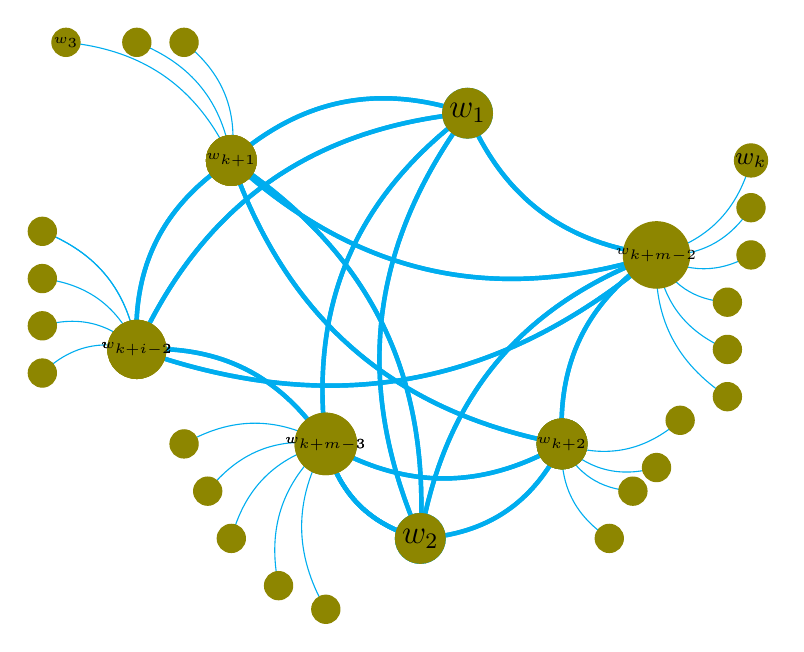
\begin{tikzpicture}[scale=0.3]

\draw[-,>=latex,ultra thick,color=cyan] (14,2) to [bend left] (10,6);
\draw[-,>=latex,ultra thick,color=cyan] (14,2) to [bend right] (20,6);
\draw[-,>=latex,ultra thick,color=cyan] (10,6) to [bend right] (2,10);
\draw[-, >=latex,ultra thick,color=cyan] (2,10) to [bend left] (6,18);
\draw[-, >=latex,ultra thick,>=latex,ultra thick,color=cyan] (20,6) to [bend left] (24,14);
\draw[-,>=latex,ultra thick, >=latex,ultra thick,color=cyan] (6,18) to [bend left] (16,20);
%\draw[-,color=cyan] (16,20) to [bend rigth] (24,14);
\draw[-,>=latex,ultra thick,color=cyan] (16,20) to [bend right] (24,14);

\draw[-,>=latex,ultra thick,color=cyan] (16,20) to [bend right] (2,10);
\draw[-,>=latex,ultra thick,color=cyan] (16,20) to [bend right] (10,6);
\draw[-,>=latex,ultra thick,color=cyan] (6,18) to [bend left] (14,2);
\draw[-, >=latex,ultra thick,color=cyan] (2,10) to [bend right] (24,14);
\draw[-, >=latex,ultra thick,color=cyan] (10,6) to [bend right] (20,6);
\draw[-,>=latex,ultra thick,color=cyan] (24,14) to [bend right] (14,2);
\draw[-,>=latex,ultra thick,color=cyan] (16,20) to [bend right] (14,2);
\draw[-,>=latex,ultra thick,color=cyan] (6,18) to [bend right] (20,6);
\draw[-,>=latex,ultra thick,color=cyan] (6,18) to [bend right] (24,14);
\draw[-, >=latex,ultra thick,color=cyan] (10,6) to [bend right] (14,2);



\filldraw[color=cyan] (14,2) circle (30pt) node[] {\large \textcolor{black}{$v_2$}};
\filldraw[color=cyan] (10,6) circle (30pt)node[] {\large \textcolor{black}{\tiny{$v_{m-1}$}}};;
 \filldraw[color=cyan] (20,6) circle (30pt)node[] {\large \textcolor{black}{$v_4$}};;
 \filldraw[color=cyan] (2,10) circle (25pt)node[] {\large \textcolor{black}{$v_i$}}; 
 \filldraw[color=cyan] (6,18) circle (25pt)node[] {\large \textcolor{black}{$v_3$}};;
 \filldraw[color=cyan] (24,14) circle (25pt)node[] {\large \textcolor{black}{$v_m$}};;
\filldraw[color=cyan] (16,20) circle (30pt) node[] {\large \textcolor{black}{$v_1$}};

\pause
%%%%%%%%%%%%%%%%%%%%%%%%%%%%%%%%%%%%%%



\draw[-,>=latex,ultra thick,color=cyan] (14,2) to [bend left] (10,6);
\draw[-,>=latex,ultra thick,color=cyan] (14,2) to [bend right] (20,6);
\draw[-,>=latex,ultra thick,color=cyan] (10,6) to [bend right] (2,10);
\draw[-, >=latex,ultra thick,color=cyan] (2,10) to [bend left] (6,18);
\draw[-, >=latex,ultra thick,>=latex,ultra thick,color=cyan] (20,6) to [bend left] (24,14);
\draw[-,>=latex,ultra thick, >=latex,ultra thick,color=cyan] (6,18) to [bend left] (16,20);
%\draw[-,color=cyan] (16,20) to [bend rigth] (24,14);
\draw[-,>=latex,ultra thick,color=cyan] (16,20) to [bend right] (24,14);

\draw[-,>=latex,ultra thick,color=cyan] (16,20) to [bend right] (2,10);
\draw[-,>=latex,ultra thick,color=cyan] (16,20) to [bend right] (10,6);
\draw[-,>=latex,ultra thick,color=cyan] (6,18) to [bend left] (14,2);
\draw[-, >=latex,ultra thick,color=cyan] (2,10) to [bend right] (24,14);
\draw[-, >=latex,ultra thick,color=cyan] (10,6) to [bend right] (20,6);
\draw[-,>=latex,ultra thick,color=cyan] (24,14) to [bend right] (14,2);
\draw[-,>=latex,ultra thick,color=cyan] (16,20) to [bend right] (14,2);
\draw[-,>=latex,ultra thick,color=cyan] (6,18) to [bend right] (20,6);
\draw[-,>=latex,ultra thick,color=cyan] (6,18) to [bend right] (24,14);
\draw[-, >=latex,ultra thick,color=cyan] (10,6) to [bend right] (14,2);





\filldraw[color=cyan] (14,2) circle (30pt) node[] {\large \textcolor{black}{$v_2$}};
\filldraw[color=cyan] (10,6) circle (30pt)node[] {\large \textcolor{black}{\tiny{$v_{m-1}$}}};;
 \filldraw[color=cyan] (20,6) circle (30pt)node[] {\large \textcolor{black}{$v_4$}};;
 \filldraw[color=cyan] (2,10) circle (25pt)node[] {\large \textcolor{black}{$v_i$}}; 
 \filldraw[color=cyan] (6,18) circle (25pt)node[] {\large \textcolor{black}{$v_3$}};;
 \filldraw[color=cyan] (24,14) circle (25pt)node[] {\large \textcolor{black}{$v_m$}};;
\filldraw[color=olive] (16,20) circle (30pt) node[] {\large \textcolor{black}{$w_1$}};
\pause
\filldraw[color=olive] (14,2) circle (30pt) node[] {\large \textcolor{black}{$w_2$}};
\pause


\draw[-,color=cyan] (6,18) to [bend right](-1,23);
\draw[-,color=cyan] (6,18) to [bend right] (2,23);
\draw[-,color=cyan] (6,18) to [bend right] (4,23);

\filldraw[color=olive] (-1,23) circle (17pt) node[] {\tiny \textcolor{black}{$w_3$}};
\filldraw[color=olive] (2,23) circle (17pt);% node[] %{\tiny \textcolor{black}{$w_4$}};
\filldraw[color=olive] (4,23) circle (17pt);% node[] %{\tiny \textcolor{black}{$w_2$}};

\filldraw[color=olive] (6,18) circle (30pt) node[] {\tiny \textcolor{black}{$w_{k+1}$}};

\pause
\draw[-,color=cyan] (20,6) to [bend right](22,2);
\draw[-,color=cyan] (20,6) to [bend right] (23,4);
\draw[-,color=cyan] (20,6) to [bend right] (24,5);
\draw[-,color=cyan] (20,6) to [bend right] (25,7);

\filldraw[color=olive] (22,2) circle (17pt);% node[] {\tiny \textcolor{black}{$w$}};
\filldraw[color=olive] (23,4) circle (17pt);% node[] %{\tiny \textcolor{black}{$w_4$}};
\filldraw[color=olive] (24,5) circle (17pt);% node[] %{\tiny \textcolor{black}{$w_2$}};
\filldraw[color=olive] (25,7) circle (17pt);% node[] %{\tiny \textcolor{black}{$w_2$}};
\filldraw[color=olive] (6,18) circle (30pt) node[] {\tiny \textcolor{black}{$w_{k+1}$}};
\filldraw[color=olive] (20,6) circle (30pt) node[] {\tiny \textcolor{black}{$w_{k+2}$}};


\pause
\draw[-,color=cyan] (2,10) to [bend right](-2,9);
\draw[-,color=cyan] (2,10) to [bend right] (-2,11);
\draw[-,color=cyan] (2,10) to [bend right] (-2,13);
\draw[-,color=cyan] (2,10) to [bend right] (-2,15);
\draw[-,color=cyan] (2,10) to [bend right] (-2,15);

\filldraw[color=olive] (-2,9) circle (17pt);% node[] {\tiny \textcolor{black}{$w$}};
\filldraw[color=olive] (-2,11) circle (17pt);% node[] %{\tiny \textcolor{black}{$w_4$}};
\filldraw[color=olive] (-2,13) circle (17pt);% node[] %{\tiny \textcolor{black}{$w_2$}};
\filldraw[color=olive] (-2,15) circle (17pt);% node[] %{\tiny \textcolor{black}{$w_2$}};

\filldraw[color=olive] (6,18) circle (30pt) node[] {\tiny \textcolor{black}{$w_{k+1}$}};
\filldraw[color=olive] (20,6) circle (30pt) node[] {\tiny \textcolor{black}{$w_{k+2}$}};
\filldraw[color=olive] (2,10) circle (35pt) node[] {\tiny \textcolor{black}{$w_{k+i-2}$}};


\pause

\draw[-,color=cyan] (10,6) to [bend right](10,-1);
\draw[-,color=cyan] (10,6) to [bend right] (8,0);
\draw[-,color=cyan] (10,6) to [bend right] (6,2);
\draw[-,color=cyan] (10,6) to [bend right] (5,4);
\draw[-,color=cyan] (10,6) to [bend right] (4,6);
\filldraw[color=olive] (10,-1) circle (17pt);% node[] {\tiny \textcolor{black}{$w$}};
\filldraw[color=olive] (8,0) circle (17pt);% node[] %{\tiny \textcolor{black}{$w_4$}};
\filldraw[color=olive] (6,2) circle (17pt);% node[] %{\tiny \textcolor{black}{$w_2$}};
\filldraw[color=olive] (5,4) circle (17pt);% node[] %{\tiny \textcolor{black}{$w_2$}};
\filldraw[color=olive] (4,6) circle (17pt);% node[] %{\tiny \textcolor{black}{$w_2$}};


\filldraw[color=olive] (6,18) circle (30pt) node[] {\tiny \textcolor{black}{$w_{k+1}$}};
\filldraw[color=olive] (20,6) circle (30pt) node[] {\tiny \textcolor{black}{$w_{k+2}$}};
\filldraw[color=olive] (2,10) circle (35pt) node[] {\tiny \textcolor{black}{$w_{k+i-2}$}};

\filldraw[color=olive] (10,6) circle (37pt) node[] {\tiny \textcolor{black}{$w_{k+m-3}$}};

\pause
\draw[-,color=cyan] (24,14) to [bend right](27,8);
\draw[-,color=cyan] (24,14) to [bend right] (27,10);
\draw[-,color=cyan] (24,14) to [bend right] (27,12);
\draw[-,color=cyan] (24,14) to [bend right] (28,14);
\draw[-,color=cyan] (24,14) to [bend right] (28,16);
\draw[-,color=cyan] (24,14) to [bend right] (28,18);

\filldraw[color=olive] (27,8) circle (17pt);% node[] {\tiny \textcolor{black}{$w$}};
\filldraw[color=olive] (27,10) circle (17pt);% node[] %{\tiny \textcolor{black}{$w_4$}};
\filldraw[color=olive] (27,12) circle (17pt);% node[] %{\tiny \textcolor{black}{$w_2$}};
\filldraw[color=olive] (28,14) circle (17pt);% node[] %{\tiny \textcolor{black}{$w_2$}};
\filldraw[color=olive] (28,16) circle (17pt);% node[] %{\tiny \textcolor{black}{$w_2$}};
\filldraw[color=olive] (28,18) circle (20pt) node[] {\small \textcolor{black}{$w_k$}};


\filldraw[color=olive] (6,18) circle (30pt) node[] {\tiny \textcolor{black}{$w_{k+1}$}};
\filldraw[color=olive] (20,6) circle (30pt) node[] {\tiny \textcolor{black}{$w_{k+2}$}};
\filldraw[color=olive] (2,10) circle (35pt) node[] {\tiny \textcolor{black}{$w_{k+i-2}$}};
\filldraw[color=olive] (10,6) circle (37pt) node[] {\tiny \textcolor{black}{$w_{k+m-3}$}};
\filldraw[color=olive] (24,14) circle (40pt) node[] {\tiny \textcolor{black}{$w_{k+m-2}$}};
\end{tikzpicture}
%\textcolor{blue}{$T  \hspace{4 cm} T'$}
\end{center}
\end{figure}
\end{frame}

%%%%%%%%%%%%%%%%%%%%%%%%%%%%%%%%%%%%%%%%%%G_m%%%%%%%%%%%%%%%%%%%%%%%%%%%55
\begin{frame}
\frametitle{Transformaci�n $f:G_m \rightarrow G_n$}

\begin{figure}[!ht]
\begin{center}
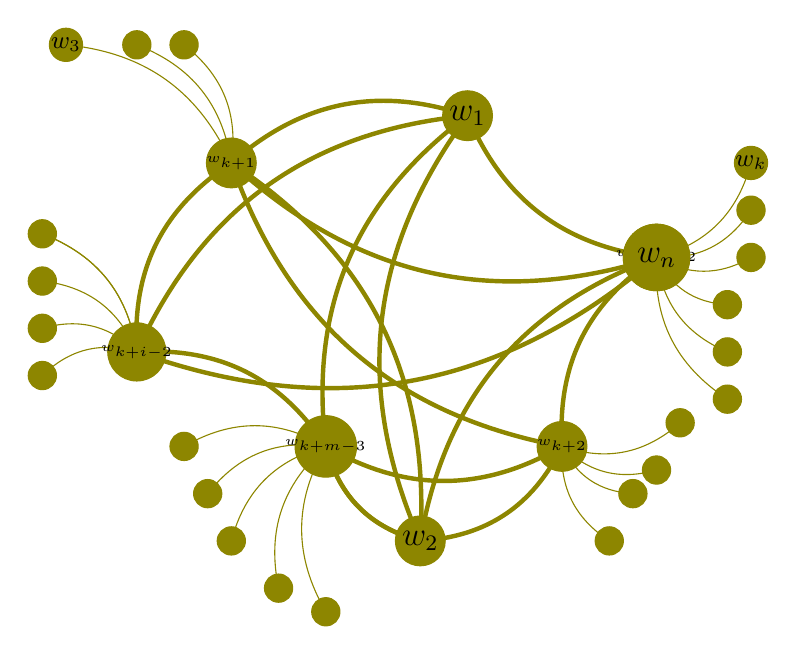
\begin{tikzpicture}[scale=0.3]

\draw[-,>=latex,ultra thick,color=olive] (14,2) to [bend left] (10,6);
\draw[-,>=latex,ultra thick,color=olive] (14,2) to [bend right] (20,6);
\draw[-,>=latex,ultra thick,color=olive] (10,6) to [bend right] (2,10);
\draw[-, >=latex,ultra thick,color=olive] (2,10) to [bend left] (6,18);
\draw[-, >=latex,ultra thick,>=latex,ultra thick,color=olive] (20,6) to [bend left] (24,14);
\draw[-,>=latex,ultra thick, >=latex,ultra thick,color=olive] (6,18) to [bend left] (16,20);
\draw[-,>=latex,ultra thick,color=olive] (16,20) to [bend right] (24,14);

\draw[-,>=latex,ultra thick,color=olive] (16,20) to [bend right] (2,10);
\draw[-,>=latex,ultra thick,color=olive] (16,20) to [bend right] (10,6);
\draw[-,>=latex,ultra thick,color=olive] (6,18) to [bend left] (14,2);
\draw[-, >=latex,ultra thick,color=olive] (2,10) to [bend right] (24,14);
\draw[-, >=latex,ultra thick,color=olive] (10,6) to [bend right] (20,6);
\draw[-,>=latex,ultra thick,color=olive] (24,14) to [bend right] (14,2);
\draw[-,>=latex,ultra thick,color=olive] (16,20) to [bend right] (14,2);
\draw[-,>=latex,ultra thick,color=olive] (6,18) to [bend right] (20,6);
\draw[-,>=latex,ultra thick,color=olive] (6,18) to [bend right] (24,14);
\draw[-, >=latex,ultra thick,color=olive] (10,6) to [bend right] (14,2);





\draw[-,color=olive] (6,18) to [bend right](-1,23);
\draw[-,color=olive] (6,18) to [bend right] (2,23);
\draw[-,color=olive] (6,18) to [bend right] (4,23);




\draw[-,color=olive] (20,6) to [bend right](22,2);
\draw[-,color=olive] (20,6) to [bend right] (23,4);
\draw[-,color=olive] (20,6) to [bend right] (24,5);
\draw[-,color=olive] (20,6) to [bend right] (25,7);


\draw[-,color=olive] (2,10) to [bend right](-2,9);
\draw[-,color=olive] (2,10) to [bend right] (-2,11);
\draw[-,color=olive] (2,10) to [bend right] (-2,13);
\draw[-,color=olive] (2,10) to [bend right] (-2,15);
\draw[-,color=olive] (2,10) to [bend right] (-2,15);




\draw[-,color=olive] (10,6) to [bend right](10,-1);
\draw[-,color=olive] (10,6) to [bend right] (8,0);
\draw[-,color=olive] (10,6) to [bend right] (6,2);
\draw[-,color=olive] (10,6) to [bend right] (5,4);
\draw[-,color=olive] (10,6) to [bend right] (4,6);




\draw[-,color=olive] (24,14) to [bend right](27,8);
\draw[-,color=olive] (24,14) to [bend right] (27,10);
\draw[-,color=olive] (24,14) to [bend right] (27,12);
\draw[-,color=olive] (24,14) to [bend right] (28,14);
\draw[-,color=olive] (24,14) to [bend right] (28,16);
\draw[-,color=olive] (24,14) to [bend right] (28,18);



\filldraw[color=olive] (-1,23) circle (20pt) node[] {\small \textcolor{black}{$w_3$}};
\filldraw[color=olive] (2,23) circle (17pt);% node[] %{\tiny \textcolor{black}{$w_4$}};
\filldraw[color=olive] (4,23) circle (17pt);% node[] %{\tiny \textcolor{black}{$w_2$}};


\filldraw[color=olive] (-2,9) circle (17pt);% node[] {\tiny \textcolor{black}{$w$}};
\filldraw[color=olive] (-2,11) circle (17pt);% node[] %{\tiny \textcolor{black}{$w_4$}};
\filldraw[color=olive] (-2,13) circle (17pt);% node[] %{\tiny \textcolor{black}{$w_2$}};
\filldraw[color=olive] (-2,15) circle (17pt);% node[] %{\tiny \textcolor{black}{$w_2$}};

\filldraw[color=olive] (10,-1) circle (17pt);% node[] {\tiny \textcolor{black}{$w$}};
\filldraw[color=olive] (8,0) circle (17pt);% node[] %{\tiny \textcolor{black}{$w_4$}};
\filldraw[color=olive] (6,2) circle (17pt);% node[] %{\tiny \textcolor{black}{$w_2$}};
\filldraw[color=olive] (5,4) circle (17pt);% node[] %{\tiny \textcolor{black}{$w_2$}};
\filldraw[color=olive] (4,6) circle (17pt);% node[] %{\tiny \textcolor{black}{$w_2$}};



\filldraw[color=olive] (22,2) circle (17pt);% node[] {\tiny \textcolor{black}{$w$}};
\filldraw[color=olive] (23,4) circle (17pt);% node[] %{\tiny \textcolor{black}{$w_4$}};
\filldraw[color=olive] (24,5) circle (17pt);% node[] %{\tiny \textcolor{black}{$w_2$}};
\filldraw[color=olive] (25,7) circle (17pt);% node[] %{\tiny \textcolor{black}{$w_2$}};


%\filldraw[color=olive] (6,18) circle (30pt) node[] {\tiny \textcolor{black}{$w_{k+1}$}};
%\filldraw[color=olive] (20,6) circle (30pt) node[] {\tiny \textcolor{black}{$w_{k+2}$}};






\filldraw[color=olive] (27,8) circle (17pt);% node[] {\tiny \textcolor{black}{$w$}};
\filldraw[color=olive] (27,10) circle (17pt);% node[] %{\tiny \textcolor{black}{$w_4$}};
\filldraw[color=olive] (27,12) circle (17pt);% node[] %{\tiny \textcolor{black}{$w_2$}};
\filldraw[color=olive] (28,14) circle (17pt);% node[] %{\tiny \textcolor{black}{$w_2$}};
\filldraw[color=olive] (28,16) circle (17pt);% node[] %{\tiny \textcolor{black}{$w_2$}};



\filldraw[color=olive] (16,20) circle (30pt) node[] {\large \textcolor{black}{$w_1$}};
\filldraw[color=olive] (14,2) circle (30pt) node[] {\large \textcolor{black}{$w_2$}};
\filldraw[color=olive] (28,18) circle (20pt) node[] {\small \textcolor{black}{$w_k$}};
\filldraw[color=olive] (6,18) circle (30pt) node[] {\tiny \textcolor{black}{$w_{k+1}$}};
\filldraw[color=olive] (20,6) circle (30pt) node[] {\tiny \textcolor{black}{$w_{k+2}$}};
\filldraw[color=olive] (2,10) circle (35pt) node[] {\tiny \textcolor{black}{$w_{k+i-2}$}};
\filldraw[color=olive] (10,6) circle (37pt) node[] {\tiny \textcolor{black}{$w_{k+m-3}$}};
\filldraw[color=olive] (24,14) circle (40pt) node[] {\tiny \textcolor{black}{$w_{k+m-2}$}};
\pause
\filldraw[color=olive] (24,14) circle (40pt) node[] {\large \textcolor{black}{$w_{n}$}};



\end{tikzpicture}
\end{center}
\end{figure}
\end{frame}


%%%%%%%%%%%%%%%%%%%%%%%%%%%%%%%%%%%%%%%%%%%%%%%%%%%%%%%%%%%%%%%%%%%%%%%%%%%%%
%
%\begin{frame}
%\frametitle{Presentaci�n de la transformaci�n $\varphi$}
%\textcolor{blue} {�Qu� es lo que hace $\varphi(T, u, v)$?}
%
%\begin{figure}[!ht]
%\begin{center}
%\begin{tikzpicture}[scale=0.3]
% \filldraw[color=black] (2,2) circle (2pt);
% \filldraw[color=blue] (4,0) circle (3pt) node[below] {\normalsize {$u$}}; %punto etiquetado
% \filldraw[color=blue] (4,2) circle (3pt);
% \filldraw[color=black] (4,4) circle (2pt); 
% \filldraw[color=blue] (6,4) circle (3pt);
% \filldraw[color=black] (8,2) circle (2pt);
% \filldraw[color=blue] (8,6) circle (3pt);
%  \filldraw[color=black] (8,8) circle (2pt);
% \filldraw[color=blue] (10,4) circle (3pt) node[above] {\normalsize {$v$}};  
%  \filldraw[color=black] (10,8) circle (2pt); 
%  \filldraw[color=black] (12,2) circle (2pt); 
%  \filldraw[color=black] (12,6) circle (2pt);
%  \filldraw[color=black] (8,6) circle (2pt);
%
%%%%%%%%%%%%%%%%%%%%%%%%%%%%%%%%%%%%%%%%%%%%%%%%%%%%%%%%%%
%
%%aristas de u a los vertices en T_u
%\draw[-, >=latex, color=blue] (4,0) to (4,2);
%\draw[-, >=latex] (4,2) to (2,2);
%\draw[-, >=latex, color=blue] (4,2) to (6,4);
%\draw[-, >=latex] (6,4) to (4,4);
%\draw[-, >=latex, color=blue] (6,4) to (8,6);
%\draw[-, >=latex, color=blue] (10,4) to (8,6);
%\draw[-, >=latex] (8,2) to (10,4);
%\draw[-, >=latex] (12,2) to (10,4);
%\draw[-, >=latex] (8,6) to (10,8);
%\draw[-, >=latex] (8,8) to (10,8);
%\draw[-, >=latex] (12,6) to (10,8);
%
%
%
%%%%%%%%%%%%%%%%%%%%%%%%%%%%%%%%%%%%%%%%%%%%%%%%%%%%%%%%
%%%%%%%%%%%%%%%%%%%%%%%%%%%%%%%%%%%%%%%%%%%%%
%
%
%\filldraw[color=black] (20,2) circle (2pt);
% \filldraw[color=blue] (22,0) circle (3pt) node[below] {\normalsize {$u$}}; %punto etiquetado
% \filldraw[color=black] (22,2) circle (2pt);
% \filldraw[color=black] (22,4) circle (2pt); 
% \filldraw[color=black] (24,4) circle (2pt);
% \filldraw[color=blue] (26,2) circle (3pt);
% \filldraw[color=black] (26,6) circle (2pt);
% \filldraw[color=black] (26,8) circle (2pt);
% \filldraw[color=black] (28,4) circle (2pt)node[above] {\normalsize {$v$}};  
%  \filldraw[color=black] (28,8) circle (2pt); 
%  \filldraw[color=blue] (30,2) circle (3pt);
%  \filldraw[color=black] (30,6) circle (2pt);
% 
%\draw[-, >=latex] (22,0) to (22,2);
%\draw[-, >=latex] (22,2) to (20,2);
%\draw[-, >=latex] (22,2) to (24,4);
%\draw[-, >=latex] (24,4) to (22,4);
%\draw[-, >=latex] (24,4) to (26,6);
%\draw[-, >=latex] (28,4) to (26,6);
%
%%\draw[dashed, >=latex] (26,2) to (28,4);
%%\draw[dashed, >=latex] (30,2) to (28,4);
%\draw[-, >=latex] (26,6) to (28,8);
%\draw[-, >=latex] (26,8) to (28,8);
%\draw[-, >=latex] (30,6) to (28,8);
%\draw[-,color=blue] (22,0) to [bend left] (26,2);
%\draw[-,color=blue] (22,0) to [bend right] (30,2);
%%%%%%%%%%%%%%%%%%%%%%%%%%%%%%%%%%%%%%%%%%%%%%%%%%%%%%%%%%%%%%%%%
%%%%%%%%%%%%%%%%%%%%%%%%%%%%%%%%%%%%%%%%%%%%%%%%%%%%%%%%%%%%%%%%%%%%
%
%\end{tikzpicture}
%\end{center}
%\textcolor{blue}{$T  \hspace{4 cm} T'$}
%\end{figure}
%\end{frame}
%
%%%%%%%%%%%%%%%%%%%%%%%%%%%%%%%%%%%%%%Inversa de la transformaci�n%%%%%%%%%%%%%%%%%%%%%%%%%%%%%555
%\begin{frame}
%\frametitle{Presentaci�n de la transformaci�n $\varphi$}
%\begin{figure}[!ht]
%\begin{center}
%%\raggedleft
%\textcolor{red}{$\varphi(T',v,u)=T$}
%\begin{tikzpicture}[scale=0.3]
% \filldraw[color=black] (2,2) circle (2pt);
% \filldraw[color=black] (4,0) circle (3pt) node[below] {\tiny {$u$}}; %punto etiquetado
% \filldraw[color=black] (4,2) circle (3pt);
% \filldraw[color=black] (4,4) circle (2pt); 
% \filldraw[color=black] (6,4) circle (3pt);
% \filldraw[color=black] (8,2) circle (2pt);
% \filldraw[color=black] (8,6) circle (3pt);
%  \filldraw[color=black] (8,8) circle (2pt);
% \filldraw[color=black] (10,4) circle (3pt) node[above] {\tiny {$v$}};  
%  \filldraw[color=black] (10,8) circle (2pt); 
%  \filldraw[color=black] (12,2) circle (2pt); 
%  \filldraw[color=black] (12,6) circle (2pt);
%  \filldraw[color=black] (8,6) circle (2pt);
%
%%%%%%%%%%%%%%%%%%%%%%%%%%%%%%%%%%%%%%%%%%%%%%%%%%%%%%%%%%
%
%%aristas de u a los vertices en T_u
%\draw[-, >=latex] (4,0) to (4,2);
%\draw[-, >=latex] (4,2) to (2,2);
%\draw[-, >=latex] (4,2) to (6,4);
%\draw[-, >=latex] (6,4) to (4,4);
%\draw[-, >=latex] (6,4) to (8,6);
%\draw[-, >=latex] (10,4) to (8,6);
%%\draw[-, >=latex] (8,2) to (10,4);
%
%%\draw[-, >=latex] (12,2) to (10,4);
%\draw[-, >=latex] (8,6) to (10,8);
%\draw[-, >=latex] (8,8) to (10,8);
%\draw[-, >=latex] (12,6) to (10,8);
%
%\draw[-, >=latex,color=blue] (4,0) to [bend right] (8,2);
%\draw[-, >=latex,color=blue] (4,0) to [bend right] (12,2);
%
%%%%%%%%%%%%%%%%%%%%%%%%%%%%%%%%%%%%%%%%%%%%%%%%%%%%%%%%
%%%%%%%%%%%%%%%%%%%%%%%%%%%%%%%%%%%%%%%%%%%%%
%
%
%\filldraw[color=black] (20,2) circle (2pt);
% \filldraw[color=blue] (22,0) circle (3pt) node[below] {\tiny {$u$}}; %punto etiquetado
% \filldraw[color=blue] (22,2) circle (2pt);
% \filldraw[color=black] (22,4) circle (2pt); 
% \filldraw[color=blue] (24,4) circle (2pt);
% \filldraw[color=blue] (26,2) circle (3pt);
% \filldraw[color=blue] (26,6) circle (2pt);
% \filldraw[color=black] (26,8) circle (2pt);
% \filldraw[color=black] (28,4) circle (2pt)node[above] {\tiny {$v$}};  
%  \filldraw[color=black] (28,8) circle (2pt); 
%  \filldraw[color=blue] (30,2) circle (3pt);
%  \filldraw[color=black] (30,6) circle (2pt);
% 
%\draw[-, >=latex, color=blue] (22,0) to (22,2);
%\draw[-, >=latex] (22,2) to (20,2);
%\draw[-, >=latex,color=blue] (22,2) to (24,4);
%\draw[-, >=latex] (24,4) to (22,4);
%\draw[-, >=latex, color=blue] (24,4) to (26,6);
%\draw[-, >=latex,color=blue] (28,4) to (26,6);
%
%\draw[-, >=latex, color=blue] (26,2) to (28,4);
%\draw[-, >=latex, color=blue] (30,2) to (28,4);
%\draw[-, >=latex] (26,6) to (28,8);
%\draw[-, >=latex] (26,8) to (28,8);
%\draw[-, >=latex] (30,6) to (28,8);
%\draw[dashed,color=black] (22,0) to [bend left] (26,2);
%\draw[dashed,color=black] (22,0) to [bend right] (30,2);
%%%%%%%%%%%%%%%%%%%%%%%%%%%%%%%%%%%%%%%%%%%%%%%%%%%%%%%%%%%%%%%%%
%%%%%%%%%%%%%%%%%%%%%%%%%%%%%%%%%%%%%%%%%%%%%%%%%%%%%%%%%%%%%%%%%%%%
%
%\end{tikzpicture}
%\textcolor{blue}{$T'  \hspace{4 cm} T$}
%\end{center}
%
%\end{figure}
%\end{frame}
%
%%%%%%%%%%%%%%%%%%%%%%%%%%%%%%%%%%%%%%%%%%%%%%%%%%%%%%55
%
%%\begin{frame}
%%\center
%%\textcolor{blue}{Algunos resultados de $\varphi$}
%%\end{frame}
%
%%%%%%%%%%%%%%%%%%%%%%%%%%%%%%%%%%%%%%%%%%%%%%%%%%%%%%%%%%%%%%%%%%%%%%%%%%%%%%%%%55
%\section{Propiedades de la transformaci�n $\varphi$}
%\begin{frame}
%\frametitle{Propiedades de la transformaci�n $\varphi$}
%\begin{block}{Lema 1.}\label{lem_intVertices}
%
%Sean \textcolor{blue}{$T$} un �rbol en \textcolor{blue}{$\mathcal{T}$} y  \textcolor{blue}{$u$} y \textcolor{blue}{$v$} v�rtices \textcolor{blue}  {adyacentes} en \textcolor{blue}{$T$} y sea \textcolor{blue}{$T'$} el �rbol isomorfo a \textcolor{blue}{$T$} que resulta del intercambio de los v�rtices \textcolor{blue}{$u$} y \textcolor{blue}{$v$}. Entonces es posible transformar \textcolor{blue}{$T$} en \textcolor{blue}{$T'$} aplicando una o tres veces sucesivas la transformaci�n \textcolor{blue}{ $\varphi$}
%
%
%\begin{figure}[!ht]
%\begin{center}
%\begin{tikzpicture}[scale=0.3]
%
% \filldraw[color=black] (0,1) circle (2pt); 
% \filldraw[color=black] (4,1) circle (2pt); 
% \filldraw[color=black] (2,3) circle (2pt);
% \filldraw[color=black] (6,3) circle (2pt);
% \filldraw[color=blue] (4,7) circle (3pt) node[above] {\normalsize {$u$}}; 
% \filldraw[color=blue] (4,5) circle (3pt) node[below ] {\normalsize {$v$}}; 
% \filldraw[color=black] (2,9) circle (2pt);   
% \filldraw[color=black] (6,9) circle (2pt);    
% \filldraw[color=black] (4,11) circle (2pt);    
%\filldraw[color=black] (8,11) circle (2pt); 
%\filldraw[color=black] (0,7) circle (2pt); 
%\filldraw[color=black] (0,11) circle (2pt); 
%%%%%%%%%%%%%%%%%%%%%%%%%%%%%%%%%%%%%%%%%%%%%%%%%%%%%%%%%%
%
%\draw[-, >=latex] (0,1) to (2,3); %arista
%\draw[-, >=latex] (4,1) to (2,3);
%\draw[-, >=latex] (2,3) to (4,5);
%\draw[-, >=latex] (6,3) to (4,5);
%\draw[-, >=latex] (4,5) to (4,7);
%\draw[-, >=latex] (4,7) to (2,9);
%\draw[-, >=latex] (4,7) to (6,9);
%\draw[-, >=latex] (6,9) to (4,11);
%\draw[-, >=latex] (6,9) to (8,11);
%\draw[-, >=latex] (2,9) to (0,11);
%\draw[-, >=latex] (2,9) to (0,7);
%
%%\newline \hspace{1cm}\textcolor {blue}{$T$} 
%%%%%%%%%%%%%%%%%%%%%%%%%%%%%%%%%%%%%%%%%%%%%%%%%%%%%%%%%%%%%%%%%%%%%%%%%%%%%%%%%%%%%%%%%%%%%%%%%%%5555
%
%
%\filldraw[color=black] (12,1) circle (2pt); 
%\filldraw[color=black] (16,1) circle (2pt); 
%\filldraw[color=black] (14,3) circle (2pt);
%\filldraw[color=black] (18,3) circle (2pt);
%\filldraw[color=blue] (16,5) circle (3pt) node[below] {\normalsize {$u$}}; 
%\filldraw[color=blue] (16,7) circle (3pt) node[above ] {\normalsize {$v$}}; 
%\filldraw[color=black] (14,9) circle (2pt) ;  
%\filldraw[color=black] (18,9) circle (2pt);  
%\filldraw[color=black] (16,11) circle (2pt);  
%\filldraw[color=black] (20,11) circle (2pt);
%\filldraw[color=black] (12,7) circle (2pt);
%\filldraw[color=black] (12,11) circle (2pt);
%
%\draw[-, >=latex] (12,1) to (14,3);
%\draw[-, >=latex] (16,1) to (14,3);
%\draw[-, >=latex] (14,3) to (16,5);
%\draw[-, >=latex] (14,3) to (16,5);
%\draw[-, >=latex] (18,3) to (16,5);
%\draw[-, >=latex] (16,5) to (16,7); % v a u
%\draw[-, >=latex] (14,9) to (16,7);
%\draw[-, >=latex] (16,7) to (18,9);
%\draw[-, >=latex] (18,9) to (16,11);
%\draw[-, >=latex] (18,9) to (20,11);
%\draw[-, >=latex] (14,9) to (12,7); 
%\draw[-, >=latex] (12,11) to (14,9);
%
%%\newline 
%%\hspace{4 cm}\textcolor {blue}{$T'$}
%
%\end{tikzpicture} \\
%\end{center}
%\end{figure}
%
%\end{block}
%\end{frame}
%%%%%%%%%%%%%%%%%%%%%%%%%%%%%%%%%%Demostraci�n del Lema 1: Caso 1%%%%%%%%%%%%%%%%%%%%%%%%%%%%%%%%%%%%%%%%%%%%%%%%%%%%%%%%%%%%%%%
%\begin{frame}
%\textcolor{blue}{\textit{Demostraci�n}}\\\
%
%\textcolor{blue}{Caso 1}. Si $d_T(u)=1$ y $d_T(v)=3$.% Entonces basta con hacer $\varphi(T, u, v)$ para obtener $T'$. 
%
%\begin{figure}[!ht]
%\begin{center}
%\begin{tikzpicture}[scale=0.4]
%
% \filldraw[color=black] (0,1) circle (2pt); %linea recta
% \filldraw[color=black] (4,1) circle (2pt); 
% \filldraw[color=black] (2,3) circle (2pt);
% \filldraw[color=black] (6,3) circle (2pt);
% \filldraw[color=black] (4,7) circle (2pt) node[above] {\normalsize {$u$}}; 
% \filldraw[color=black] (4,5) circle (2pt) node[below ] {\normalsize {$v$}}; 
%
%%%%%%%%%%%%%%%%%%%%%%%%%%%%%%%%%%%%%%%%%%%%%%%%%%%%%%%%%%
%
%%aristas de u a los vertices en T_u
%\draw[-, >=latex] (0,1) to (2,3);
%\draw[-, >=latex] (4,1) to (2,3);
%\draw[-, >=latex] (2,3) to (4,5);
%\draw[-, >=latex] (6,3) to (4,5);
%\draw[-, >=latex] (4,5) to (4,7);
%
%%%%%%%%%%%%%%%%%%%%%%%%%%%%%%%%%%%%%%%%%%%%%%%%%%%%%%%%
%%%%%%%%%%%%%%%%%%%%%%%%%%%%%%%%%%%%%%%%%%%%%
%\filldraw[color=black] (8,1) circle (2pt); 
%\filldraw[color=black] (12,1) circle (2pt); 
%\filldraw[color=black] (10,3) circle (2pt);
%\filldraw[color=black] (14,3) circle (2pt);
%\filldraw[color=black] (12,5) circle (2pt) node[below] {\normalsize {$v$}}; 
%\filldraw[color=black] (12,7) circle (2pt) node[above ] {\normalsize {$u$}}; 
%
%\draw[-, >=latex] (8,1) to (10,3);
%\draw[-, >=latex] (12,1) to (10,3);
%\draw[-, >=latex] (12,5) to (12,7);
%\draw[-, color=red] (12,7) to [bend right] (10,3);
%\draw[-, color=red] (12,7) to [bend left] (14,3);
%
%\end{tikzpicture}\\
%\textcolor {blue}{$T \hspace{3 cm} T'$} 
%\end{center}
%\end{figure}
%\end{frame}
%
%%%%%%%%%%%%%%%%%%%%%%%%%%%%%%%%Demostraci�n Lema: Caso 2%%%%%%%%%%%%%%%%%%%%%%%%%%%%%%%%%%%%%%%%%%%%
%\begin{frame}
%\textcolor{blue}{\textit{Demostraci�n}}\\\
%
%\textcolor{blue}{Caso 2}. Si $d_T(u)= d_T(v)=3$
%\begin{center}
%\begin{tikzpicture}[scale=0.4]
% \filldraw[color=black] (0,1) circle (2pt); 
% \filldraw[color=black] (4,1) circle (2pt); 
% \filldraw[color=black] (2,3) circle (2pt);
% \filldraw[color=black] (6,3) circle (2pt);
% \filldraw[color=black] (4,7) circle (2pt) node[above] {\normalsize {$u$}}; 
% \filldraw[color=black] (4,5) circle (2pt) node[below ] {\normalsize {$v$}}; 
% \filldraw[color=black] (2,9) circle (2pt);   
% \filldraw[color=black] (6,9) circle (2pt);    
% \filldraw[color=black] (4,11) circle (2pt);    
%\filldraw[color=black] (8,11) circle (2pt); 
%\filldraw[color=black] (0,7) circle (2pt); 
%\filldraw[color=black] (0,11) circle (2pt); 
%%%%%%%%%%%%%%%%%%%%%%%%%%%%%%%%%%%%%%%%%%%%%%%%%%%%%%%%%%
%
%\draw[-, >=latex] (0,1) to (2,3); %arista
%\draw[-, >=latex] (4,1) to (2,3);
%\draw[-, >=latex] (2,3) to (4,5);
%\draw[-, >=latex] (6,3) to (4,5);
%\draw[-, >=latex] (4,5) to (4,7);
%\draw[-, >=latex] (4,7) to (2,9);
%\draw[-, >=latex] (4,7) to (6,9);
%\draw[-, >=latex] (6,9) to (4,11);
%\draw[-, >=latex] (6,9) to (8,11);
%\draw[-, >=latex] (2,9) to (0,11);
%\draw[-, >=latex] (2,9) to (0,7);
%
%
%%%%%%%%%%%%%%%%%%%%%Caso 2. Figura 2   %%%%%%%%%%%%%%%%%%%%%%%%
%\filldraw[color=black] (12,1) circle (2pt)node[below] {\normalsize {$z$}}; 
%\filldraw[color=black] (16,1) circle (2pt); 
%\filldraw[color=black] (14,3) circle (2pt);
%\filldraw[color=black] (18,3) circle (2pt);
%\filldraw[color=black] (16,5) circle (2pt) node[below] {\normalsize {$v$}}; 
%\filldraw[color=black] (16,7) circle (2pt) node[above ] {\normalsize {$u$}}; 
%\filldraw[color=black] (14,9) circle (2pt) ;  
%\filldraw[color=black] (18,9) circle (2pt);  
%\filldraw[color=black] (16,11) circle (2pt);  
%\filldraw[color=black] (20,11) circle (2pt);
%\filldraw[color=black] (12,7) circle (2pt);
%\filldraw[color=black] (12,11) circle (2pt);
%
%\draw[-, >=latex] (12,1) to (14,3);%aristas
%\draw[-, >=latex] (16,1) to (14,3);
%\draw[-, >=latex] (14,3) to (16,5);
%\draw[-, >=latex] (14,3) to (16,5);
%\draw[-, >=latex] (18,3) to (16,5);
%\draw[dashed, >=latex] (16,5) to (16,7); % v a u
%\draw[-, >=latex] (14,9) to (16,7);
%\draw[-, >=latex] (16,7) to (18,9);
%\draw[-, >=latex] (18,9) to (16,11);
%\draw[-, >=latex] (18,9) to (20,11);
%\draw[-, >=latex] (14,9) to (12,7); 
%\draw[-, >=latex] (12,11) to (14,9); 
%
%\end{tikzpicture}
%\textcolor{blue}{$T  \hspace{4 cm}   T- \{uv\}$}
%\end{center}
%\end{frame}
%
%%%%%%%%%%%%%%%%%%%%%%%%%%%%%%%%%Figura 3 %%%%%%%%%%%%%%%%%%
%\begin{frame}
%\textcolor{blue}{\textit{Demostraci�n}}\\
%\begin{center}
%\begin{tikzpicture}[scale=0.4]
%\filldraw[color=black] (0,1) circle (2pt)node[below ] {\normalsize {$z$}}; 
% \filldraw[color=black] (4,1) circle (2pt); 
% \filldraw[color=black] (2,3) circle (2pt);
% \filldraw[color=black] (6,3) circle (2pt);
% \filldraw[color=black] (4,7) circle (2pt) node[above] {\normalsize {$u$}}; 
%  \filldraw[color=black] (4,5) circle (2pt) node[below ] {\normalsize {$v$}}; 
% \filldraw[color=black] (2,9) circle (2pt);   
% \filldraw[color=black] (6,9) circle (2pt);    
% \filldraw[color=black] (4,11) circle (2pt);    
%\filldraw[color=black] (8,11) circle (2pt); 
%\filldraw[color=black] (0,7) circle (2pt); 
%\filldraw[color=black] (0,11) circle (2pt); 
%
%\draw[-, >=latex] (0,1) to (2,3);%aristas
%\draw[-, >=latex] (4,1) to (2,3);
%\draw[-, >=latex] (2,3) to (4,5);
%\draw[-, >=latex] (6,3) to (4,5);
%\draw[-, >=latex] (4,5) to (4,7);
%\draw[-, >=latex] (6,9) to (4,11);
%\draw[-, >=latex] (6,9) to (8,11);
%\draw[-, >=latex] (2,9) to (0,11);
%\draw[-, >=latex] (2,9) to (0,7);
%\draw[-,  >=latex,  color = red] (0,1) to [bend right] (2,9);
%\draw[-,  >=latex,  color = red] (0,1) to [bend right] (6,9);
%
%%%%%%%%%%%%%%%Figura 4%%%%%%%%%%%%%%
%
%\filldraw[color=black] (12,1) circle (2pt)node[below] {\normalsize {$z$}}; 
%\filldraw[color=black] (16,1) circle (2pt); 
%\filldraw[color=black] (14,3) circle (2pt);
%\filldraw[color=black] (18,3) circle (2pt);
%\filldraw[color=black] (16,5) circle (2pt) node[below] {\normalsize {$v$}}; 
%\filldraw[color=black] (16,7) circle (2pt) node[above ] {\normalsize {$u$}}; 
%\filldraw[color=black] (14,9) circle (2pt);  
%\filldraw[color=black] (18,9) circle (2pt);  
%\filldraw[color=black] (16,11) circle (2pt);  
%\filldraw[color=black] (20,11) circle (2pt);
%\filldraw[color=black] (12,7) circle (2pt);
%\filldraw[color=black] (12,11) circle (2pt);
%
%
%
%\draw[-, >=latex] (12,1) to (14,3);
%\draw[-, >=latex] (16,1) to (14,3);
%\draw[-, >=latex] (16,5) to (16,7); % v a u
%\draw[-, >=latex] (18,9) to (16,11);
%\draw[-, >=latex] (18,9) to (20,11);
%\draw[-, >=latex] (14,9) to (12,7); 
%\draw[-, >=latex] (12,11) to (14,9); 
%\draw[-] (12,1) to [bend right] (14,9);
%\draw[-] (12,1) to [bend right] (18,9);
%\draw[-, >=latex,color=red] (16,7) to (14,3);
%\draw[-, >=latex, color=red] (16,7) to (18,3);
%
%\end{tikzpicture}\\
%\textcolor{blue}{$T_1= \varphi(T, z, u) \hspace{2 cm} T_2= \varphi(T_1, u, v)$ }
%\end{center}
%\end{frame}
%
%
%%%%%%%%%%%%%%%%%%%%%%%%%%%%%%%%%%%%%%%%%%%%%%%%%%%%%%%%%%%%%%%%%%55555
%\begin{frame}
%\textcolor{blue}{\textit{Demostraci�n}}\\
%\begin{figure}
%\begin{center}
%\begin{tikzpicture}[scale=0.4]
%\filldraw[color=black] (0,1) circle (2pt)node[below ] {\normalsize {$z$}}; 
%\filldraw[color=black] (4,1) circle (2pt); 
%\filldraw[color=black] (2,3) circle (2pt);
%\filldraw[color=black] (6,3) circle (2pt);
%\filldraw[color=black] (4,7) circle (2pt) node[above] {\normalsize {$u$}}; 
%\filldraw[color=black] (4,5) circle (2pt) node[below ] {\normalsize {$v$}}; 
%\filldraw[color=black] (2,9) circle (2pt);   
%\filldraw[color=black] (6,9) circle (2pt);    
%\filldraw[color=black] (4,11) circle (2pt);    
%\filldraw[color=black] (8,11) circle (2pt); 
%\filldraw[color=black] (0,7) circle (2pt); 
%\filldraw[color=black] (0,11) circle (2pt); 
%%%%%%%%%%%%%%%%%%%%%%%%%%%%%%%%%%%%%%%%%%%%%%%%%%%%%%%%%%
%
%\draw[-, >=latex] (0,1) to (2,3); %aristas
%\draw[-, >=latex] (4,1) to (2,3);
%\draw[-, >=latex] (2,3) to (4,7);
%\draw[-, >=latex] (6,3) to (4,7);
%\draw[-, >=latex] (4,5) to (4,7); %de v a u
%\draw[-, >=latex, color=red] (4,5) to (2,9);
%\draw[-, >=latex, color=red] (4,5) to (6,9);
%\draw[-, >=latex] (6,9) to (4,11);
%\draw[-, >=latex] (6,9) to (8,11);
%\draw[-, >=latex] (2,9) to (0,11);
%\draw[-, >=latex] (2,9) to (0,7);
%
%\end{tikzpicture}\\
%\textcolor{blue}{$T'= \varphi(T_2, v, z)$}
%\end{center}
%\end{figure}
%\end{frame}
%
%
%%%%%%%%%%%%%%%%%%%%%%%%%%%%%%%%%%%%%%%%%%%%%%%%%%%%%%TEOREMA 1%%%%%%%%%%%%%%%%%%%%%%%55555
%%%%%%%%%%%%%%%%%%%%%%%%%%%%%%%%%%%%%%%%%%%%%%%%%%%%
%%\section{Avances realizados}
%\begin{frame}
%%\framesubtitle{Caso $k=3$}
%\frametitle{Propiedades de la transformaci�n $\varphi$}
%\begin{block}{Teorema 1.}
%Si \textcolor{blue}{$T$} y \textcolor{blue}{$T'$} en \textcolor{blue}{$\mathcal{T}$} son isomorfos. Entonces se puede ir de \textcolor{blue}{$T$} a \textcolor{blue}{$T'$} intercambiando v�rtices adyacentes.
%\end{block}
% \end{frame}
%%%%%%%%%%%%%%%%%%%%%%%%%%%%%%%%%%%%%%%%%%%%%%%%%ELECCI�N DE RA�Z%%%%%%%%%%%%%%%%%
%
%
%\begin{frame}
%%\tiny{Elecci�n de las ra�ces en $T'$ y $T$}
%\begin{figure}[!ht]
%\begin{center}
%%\textcolor{blue}{T'}
%\begin{tikzpicture}[scale=0.3]
%
%
%
%
%%%%%%%%%Teorema1:Figura T%%%%%%%%%%%%
%\filldraw[color=red] (5,14) circle (3pt) node[above] {\normalsize {$r'$}};
%\filldraw[color=black] (3,12) circle (2pt);
%\filldraw[color=black] (5,12) circle (2pt);
%\filldraw[color=black] (7,12) circle (2pt);%
%\filldraw[color=black] (0,10) circle (2pt);
%\filldraw[color=black] (2,10) circle (2pt);
%\filldraw[color=black] (4,10) circle (2pt);
%\filldraw[color=black] (6,10) circle (2pt);
%\filldraw[color=black] (8,10) circle (2pt);
%\filldraw[color=black] (10,10) circle (2pt);%
%\filldraw[color=black] (1,8) circle (2pt);
%\filldraw[color=black] (3,8) circle (2pt);
%\filldraw[color=black] (5,8) circle (2pt);
%\filldraw[color=black] (7,8) circle (2pt);
%\filldraw[color=black] (9,8) circle (2pt);
%\filldraw[color=black] (11,8) circle (2pt);%
%\filldraw[color=black] (2,6) circle (2pt);
%\filldraw[color=black] (4,6) circle (2pt);
%\filldraw[color=black] (10,6) circle (2pt);
%\filldraw[color=black] (12,6) circle (2pt);%
%\filldraw[color=black] (1,4) circle (2pt);
%\filldraw[color=black] (3,4) circle (2pt);
%\filldraw[color=black] (9,4) circle (2pt); 
%\filldraw[color=black] (11,4) circle (2pt);
%
%
%%aristas
%\draw[-, >=latex] (5,14) to (3,12);
%\draw[-, >=latex] (5,14) to (5,12);
%\draw[-, >=latex] (5,14) to (7,12);%
%\draw[-, >=latex] (3,12) to (0,10);
%\draw[-, >=latex] (3,12) to (2,10);
%\draw[-, >=latex] (5,12) to (4,10);
%\draw[-, >=latex] (5,12) to (6,10);
%\draw[-, >=latex] (7,12) to (8,10);
%\draw[-, >=latex] (7,12) to (10,10);%
%\draw[-, >=latex] (2,10) to (1,8);
%\draw[-, >=latex] (2,10) to (3,8);
%\draw[-, >=latex] (6,10) to (5,8);
%\draw[-, >=latex] (6,10) to (7,8);
%\draw[-, >=latex] (10,10) to (9,8);
%\draw[-, >=latex] (10,10) to (11,8);%
%\draw[-, >=latex] (3,8) to (2,6);
%\draw[-, >=latex] (3,8) to (4,6);
%\draw[-, >=latex] (11,8) to (10,6);
%\draw[-, >=latex] (11,8) to (12,6);%
%\draw[-, >=latex] (2,6) to (1,4);
%\draw[-, >=latex] (2,6) to (3,4);
%\draw[-, >=latex] (10,6) to (9,4);
%\draw[-, >=latex] (10,6) to (11,4);
%
%%%%%%%%%Teorema1:Figura2%%%%%%%%%%%%
%%\pause
%
%\filldraw[color=red] (21,14) circle (3pt) node[above] {\normalsize {$r=f(r')$}};
%\filldraw[color=black] (19,12) circle (2pt);
%\filldraw[color=black] (21,12) circle (2pt);
%\filldraw[color=black] (23,12) circle (2pt);%
%\filldraw[color=black] (16,10) circle (2pt);
%\filldraw[color=black] (18,10) circle (2pt);
%\filldraw[color=black] (20,10) circle (2pt);
%\filldraw[color=black] (22,10) circle (2pt);
%\filldraw[color=black] (24,10) circle (2pt);
%\filldraw[color=black] (26,10) circle (2pt);%%
%\filldraw[color=black] (17,8) circle (2pt);
%\filldraw[color=black] (19,8) circle (2pt);
%\filldraw[color=black] (21,8) circle (2pt);
%\filldraw[color=black] (23,8) circle (2pt);
%\filldraw[color=black] (25,8) circle (2pt);
%\filldraw[color=black] (27,8) circle (2pt);%
%\filldraw[color=black] (18,6) circle (2pt);
%\filldraw[color=black] (20,6) circle (2pt);
%\filldraw[color=black] (26,6) circle (2pt);
%\filldraw[color=black] (28,6) circle (2pt);%
%\filldraw[color=black] (17,4) circle (2pt);
%\filldraw[color=black] (19,4) circle (2pt);
%\filldraw[color=black] (25,4) circle (2pt);
%\filldraw[color=black] (27,4) circle (2pt);
%
%
%%aristas
%\draw[-, >=latex] (21,14) to (19,12);
%\draw[-, >=latex] (21,14) to (21,12);
%\draw[-, >=latex] (21,14) to (23,12);%
%\draw[-, >=latex] (19,12) to (16,10);
%\draw[-, >=latex] (19,12) to (18,10);
%\draw[-, >=latex] (21,12) to (20,10);
%\draw[-, >=latex] (21,12) to (22,10);
%\draw[-, >=latex] (23,12) to (24,10);
%\draw[-, >=latex] (23,12) to (26,10);%
%\draw[-, >=latex] (18,10) to (17,8);
%\draw[-, >=latex] (18,10) to (19,8);
%\draw[-, >=latex] (22,10) to (21,8);
%\draw[-, >=latex] (22,10) to (23,8);
%\draw[-, >=latex] (26,10) to (25,8);
%\draw[-, >=latex] (26,10) to (27,8);%
%\draw[-, >=latex] (19,8) to (18,6);
%\draw[-, >=latex] (19,8) to (20,6);
%\draw[-, >=latex] (27,8) to (26,6);
%\draw[-, >=latex] (27,8) to (28,6);%
%\draw[-, >=latex] (18,6) to (17,4);
%\draw[-, >=latex] (18,6) to (19,4);
%\draw[-, >=latex] (26,6) to (25,4);
%\draw[-, >=latex] (26,6) to (27,4);
%
%\end{tikzpicture}
%
%\end{center}
%\vspace{1 cm}
%\textcolor{blue}{ $f:T' \rightarrow T$}
%\end{figure}
%\end{frame}
%%%%%%%%%%%%%%%%%%%%%%%%%%%%%%%%%%%%%%%%%%ELECCION DE v en nivel m�s bajo de T'  %%%%%%%%%%%%%%%%%%%%%%%%%%
%\begin{frame}
%%\tiny{Elecci�n de $v$ en $T'$ en el nivel $N$}
%\begin{figure}[!ht]
%\begin{center}
%\begin{tikzpicture}[scale=0.3]
%%%%%%%%%Teorema1:Figura T%%%%%%%%%%%%
%\filldraw[color=black] (5,14) circle (2pt) node[above] {\normalsize {$r'$}};
%\filldraw[color=black] (3,12) circle (2pt);
%\filldraw[color=black] (5,12) circle (2pt);
%\filldraw[color=black] (7,12) circle (2pt);%
%\filldraw[color=black] (0,10) circle (2pt);
%\filldraw[color=black] (2,10) circle (2pt);
%\filldraw[color=black] (4,10) circle (2pt);
%\filldraw[color=black] (6,10) circle (2pt);
%\filldraw[color=black] (8,10) circle (2pt);
%\filldraw[color=black] (10,10) circle (2pt);%
%\filldraw[color=black] (1,8) circle (2pt);
%\filldraw[color=black] (3,8) circle (2pt);
%\filldraw[color=black] (5,8) circle (2pt);
%\filldraw[color=black] (7,8) circle (2pt) ;
%\filldraw[color=black] (9,8) circle (2pt);
%\filldraw[color=black] (11,8) circle (2pt);%
%\filldraw[color=black] (2,6) circle (2pt);
%\filldraw[color=black] (4,6) circle (2pt);
%\filldraw[color=black] (10,6) circle (2pt);
%\filldraw[color=black] (12,6) circle (2pt);%
%\filldraw[color=black] (1,4) circle (2pt);
%\filldraw[color=black] (3,4) circle (2pt);
%\filldraw[color=red] (9,4) circle (3pt)node[below] {\small {$v$}};
%\filldraw[color=black] (11,4) circle (2pt);
%
%
%%aristas
%\draw[-, >=latex] (5,14) to (3,12);
%\draw[-, >=latex] (5,14) to (5,12);
%\draw[-, >=latex] (5,14) to (7,12);%
%\draw[-, >=latex] (3,12) to (0,10);
%\draw[-, >=latex] (3,12) to (2,10);
%\draw[-, >=latex] (5,12) to (4,10);
%\draw[-, >=latex] (5,12) to (6,10);
%\draw[-, >=latex] (7,12) to (8,10);
%\draw[-, >=latex] (7,12) to (10,10);%
%\draw[-, >=latex] (2,10) to (1,8);
%\draw[-, >=latex] (2,10) to (3,8);
%\draw[-, >=latex] (6,10) to (5,8);
%\draw[-, >=latex] (6,10) to (7,8);
%\draw[-, >=latex] (10,10) to (9,8);
%\draw[-, >=latex] (10,10) to (11,8);%
%\draw[-, >=latex] (3,8) to (2,6);
%\draw[-, >=latex] (3,8) to (4,6);
%\draw[-, >=latex] (11,8) to (10,6);
%\draw[-, >=latex] (11,8) to (12,6);%
%\draw[-, >=latex] (2,6) to (1,4);
%\draw[-, >=latex] (2,6) to (3,4);
%\draw[-, >=latex] (10,6) to (9,4);
%\draw[-, >=latex] (10,6) to (11,4);
%
%\end{tikzpicture}
%\end{center}
%\end{figure}
%\end{frame}
%
%%%%%%%%%Teorema1:Ubicar a f(v) en T %%%%%%%%%%%%%%%%%%%%%%%%%%%%%%%%%%%%%555555
%\begin{frame}
%\begin{figure}[!ht]
%\raggedleft
%\begin{tikzpicture}[scale=0.15]
%\tikzstyle{circulo}= [thin, dotted, ]
%\draw [circulo] (6,9) circle (8);
%
%
%%%%%%%%%Teorema1:Figura T%%%%%%%%%%%%
%\filldraw[color=black] (5,14) circle (2pt) node[above,xshift=1mm] {\tiny {$r'$}};
%\filldraw[color=black] (3,12) circle (2pt);
%\filldraw[color=black] (5,12) circle (2pt);
%\filldraw[color=black] (7,12) circle (2pt);%
%\filldraw[color=black] (0,10) circle (2pt);
%\filldraw[color=black] (2,10) circle (2pt);
%\filldraw[color=black] (4,10) circle (2pt);
%\filldraw[color=black] (6,10) circle (2pt);
%\filldraw[color=black] (8,10) circle (2pt);
%\filldraw[color=black] (10,10) circle (2pt);%
%\filldraw[color=black] (1,8) circle (2pt);
%\filldraw[color=black] (3,8) circle (2pt);
%\filldraw[color=black] (5,8) circle (2pt);
%\filldraw[color=black] (7,8) circle (2pt) ;
%\filldraw[color=black] (9,8) circle (2pt);
%\filldraw[color=black] (11,8) circle (2pt);%
%\filldraw[color=black] (2,6) circle (2pt);
%\filldraw[color=black] (4,6) circle (2pt);
%\filldraw[color=black] (10,6) circle (2pt);
%\filldraw[color=black] (12,6) circle (2pt);%
%\filldraw[color=black] (1,4) circle (2pt);
%\filldraw[color=black] (3,4) circle (2pt);
%\filldraw[color=red] (9,4) circle (3pt)node[below] {\tiny {$v$}};
%\filldraw[color=black] (11,4) circle (2pt);
%
%
%%aristas
%\draw[-, >=latex] (5,14) to (3,12);
%\draw[-, >=latex] (5,14) to (5,12);
%\draw[-, >=latex] (5,14) to (7,12);%
%\draw[-, >=latex] (3,12) to (0,10);
%\draw[-, >=latex] (3,12) to (2,10);
%\draw[-, >=latex] (5,12) to (4,10);
%\draw[-, >=latex] (5,12) to (6,10);
%\draw[-, >=latex] (7,12) to (8,10);
%\draw[-, >=latex] (7,12) to (10,10);%
%\draw[-, >=latex] (2,10) to (1,8);
%\draw[-, >=latex] (2,10) to (3,8);
%\draw[-, >=latex] (6,10) to (5,8);
%\draw[-, >=latex] (6,10) to (7,8);
%\draw[-, >=latex] (10,10) to (9,8);
%\draw[-, >=latex] (10,10) to (11,8);%
%\draw[-, >=latex] (3,8) to (2,6);
%\draw[-, >=latex] (3,8) to (4,6);
%\draw[-, >=latex] (11,8) to (10,6);
%\draw[-, >=latex] (11,8) to (12,6);%
%\draw[-, >=latex] (2,6) to (1,4);
%\draw[-, >=latex] (2,6) to (3,4);
%\draw[-, >=latex] (10,6) to (9,4);
%\draw[-, >=latex] (10,6) to (11,4);
%
%\end{tikzpicture}
%%\end{left}
%\end{figure}
%
%
%%%%%%%%%%%%%%%%%%%%%%%%%%%%%%%%%Ubicar v en el nivel N en el �rbol T,%%%%%%%%%%%%%%%%%%%%%%%%%%%%%%%%%%%%%%%%%%%%%%%%%%%%%
%%%%%%%%%%%%%%%%%%%%%%%%%%%%%%%%%Caso f(v) tiene la etiqueta de v%%%%%%%%%%%%%%%%%%%%%%%%%%%%%%%%%%%%%
%\pause
%%\tiny{Ubicar $v$ en $T$ en el nivel $N$}
%\tiny{\hspace{1cm} Caso 1. $f(v)=v$ \hspace{4cm} Caso 2. $f(v)\neq v$}
%\begin{figure}[!ht]
%
%\begin{center}
%\begin{tikzpicture}[scale=0.35]
%%%%%%%%%Teorema1:Figura T%%%%%%%%%%%%
%\filldraw[color=black] (5,14) circle (2pt) node[above] {\normalsize {$r$}};
%\filldraw[color=black] (3,12) circle (2pt);
%\filldraw[color=black] (5,12) circle (2pt);
%\filldraw[color=black] (7,12) circle (2pt);%
%\filldraw[color=black] (0,10) circle (2pt);
%\filldraw[color=black] (2,10) circle (2pt);
%\filldraw[color=black] (4,10) circle (2pt);
%\filldraw[color=black] (6,10) circle (2pt);
%\filldraw[color=black] (8,10) circle (2pt);
%\filldraw[color=black] (10,10) circle (2pt);%
%\filldraw[color=black] (1,8) circle (2pt);
%\filldraw[color=black] (3,8) circle (2pt);
%\filldraw[color=black] (5,8) circle (2pt);
%\filldraw[color=black] (7,8) circle (2pt) ;
%\filldraw[color=black] (9,8) circle (2pt);
%\filldraw[color=black] (11,8) circle (2pt);%
%\filldraw[color=black] (2,6) circle (2pt);
%\filldraw[color=black] (4,6) circle (2pt);
%\filldraw[color=black] (10,6) circle (2pt);
%\filldraw[color=black] (12,6) circle (2pt);%
%\filldraw[color=black] (1,4) circle (2pt);
%\filldraw[color=black] (3,4) circle (2pt);
%\filldraw[color=red] (9,4) circle (3pt) node[below]  {\small {$v$}};
%\filldraw[color=black] (11,4) circle (2pt);
%
%
%%aristas
%\draw[-, >=latex] (5,14) to (3,12);
%\draw[-, >=latex] (5,14) to (5,12);
%\draw[-, >=latex] (5,14) to (7,12);%
%\draw[-, >=latex] (3,12) to (0,10);
%\draw[-, >=latex] (3,12) to (2,10);
%\draw[-, >=latex] (5,12) to (4,10);
%\draw[-, >=latex] (5,12) to (6,10);
%\draw[-, >=latex] (7,12) to (8,10);
%\draw[-, >=latex] (7,12) to (10,10);%
%\draw[-, >=latex] (2,10) to (1,8);
%\draw[-, >=latex] (2,10) to (3,8);
%\draw[-, >=latex] (6,10) to (5,8);
%\draw[-, >=latex] (6,10) to (7,8);
%\draw[-, >=latex] (10,10) to (9,8);
%\draw[-, >=latex] (10,10) to (11,8);%
%\draw[-, >=latex] (3,8) to (2,6);
%\draw[-, >=latex] (3,8) to (4,6);
%\draw[-, >=latex] (11,8) to (10,6);
%\draw[-, >=latex] (11,8) to (12,6);%
%\draw[-, >=latex] (2,6) to (1,4);
%\draw[-, >=latex] (2,6) to (3,4);
%\draw[-, >=latex] (10,6) to (9,4);
%\draw[-, >=latex] (10,6) to (11,4);
%
%%%%%%%%%%%%%%%%%%%%%%%%%%%%%%%%%Ubicar v en el nivel N en el �rbol T,%%%%%%%%%%%%%%%%%%%%%%%%%%%%%%%%%%%%%%%%%%%%%%%%%%%%%
%%%%%%%%%%%%%%%%%%%%%%%%%%%%%%%%%Caso. f(v) tiene no tiene la etiqueta de v si no z%%%%%%%%%%%%%%%%%%%%%%%%%%%%%%%%%%%%%
%%\pause
%
%\filldraw[color=black] (21,14) circle (2pt) node[above] {\normalsize {$r$}};
%\filldraw[color=black] (19,12) circle (2pt);
%\filldraw[color=black] (21,12) circle (2pt);
%\filldraw[color=black] (23,12) circle (2pt);%
%\filldraw[color=black] (16,10) circle (2pt);
%\filldraw[color=black] (18,10) circle (2pt);
%\filldraw[color=black] (20,10) circle (2pt);
%\filldraw[color=black] (22,10) circle (2pt);
%\filldraw[color=black] (24,10) circle (2pt);
%\filldraw[color=black] (26,10) circle (2pt);%%
%\filldraw[color=black] (17,8) circle (2pt);
%\filldraw[color=black] (19,8) circle (2pt);
%\filldraw[color=black] (21,8) circle (2pt);
%\filldraw[color=red] (23,8) circle (2pt)node[below]  {\small {$v$}};
%\filldraw[color=black] (25,8) circle (2pt);
%\filldraw[color=black] (27,8) circle (2pt);%
%\filldraw[color=black] (18,6) circle (2pt);
%\filldraw[color=black] (20,6) circle (2pt);
%\filldraw[color=black] (26,6) circle (2pt);
%\filldraw[color=black] (28,6) circle (2pt);%
%\filldraw[color=black] (17,4) circle (2pt);
%\filldraw[color=black] (19,4) circle (2pt);
%\filldraw[color=red] (25,4) circle (2pt) node[below]  {\small {$z$}};
%\filldraw[color=black] (27,4) circle (2pt);
%
%
%%aristas
%\draw[-, >=latex] (21,14) to (19,12);
%\draw[-, >=latex] (21,14) to (21,12);
%\draw[-, >=latex] (21,14) to (23,12);%
%\draw[-, >=latex] (19,12) to (16,10);
%\draw[-, >=latex] (19,12) to (18,10);
%\draw[-, >=latex] (21,12) to (20,10);
%\draw[-, >=latex] (21,12) to (22,10);
%\draw[-, >=latex] (23,12) to (24,10);
%\draw[-, >=latex] (23,12) to (26,10);%
%\draw[-, >=latex] (18,10) to (17,8);
%\draw[-, >=latex] (18,10) to (19,8);
%\draw[-, >=latex] (22,10) to (21,8);
%\draw[-, >=latex] (22,10) to (23,8);
%\draw[-, >=latex] (26,10) to (25,8);
%\draw[-, >=latex] (26,10) to (27,8);%
%\draw[-, >=latex] (19,8) to (18,6);
%\draw[-, >=latex] (19,8) to (20,6);
%\draw[-, >=latex] (27,8) to (26,6);
%\draw[-, >=latex] (27,8) to (28,6);%
%\draw[-, >=latex] (18,6) to (17,4);
%\draw[-, >=latex] (18,6) to (19,4);
%\draw[-, >=latex] (26,6) to (25,4);
%\draw[-, >=latex] (26,6) to (27,4);
%\end{tikzpicture}
%\end{center}
%\end{figure}
%\end{frame}
%
%%%%%%%%%%%%%%%%%%%%%%%%%%%%%%%%%%%%%%%%%%%%%%%%%%%%%%%%%%%%%%%%%%%%%%%%555
%\begin{frame}
%\begin{figure}[!ht]
%\raggedleft
%\begin{tikzpicture}[scale=0.1] %circulo
%\tikzstyle{circulo}= [thin, dotted, ]
%\draw [circulo] (6,9) circle (9);
%\filldraw[color=black] (5,14) circle (2pt) node[above,xshift=1mm] {\tiny {$r'$}};
%\filldraw[color=black] (3,12) circle (2pt);
%\filldraw[color=black] (5,12) circle (2pt);
%\filldraw[color=black] (7,12) circle (2pt);%
%\filldraw[color=black] (0,10) circle (2pt);
%\filldraw[color=black] (2,10) circle (2pt);
%\filldraw[color=black] (4,10) circle (2pt);
%\filldraw[color=black] (6,10) circle (2pt);
%\filldraw[color=black] (8,10) circle (2pt);
%\filldraw[color=black] (10,10) circle (2pt);%
%\filldraw[color=black] (1,8) circle (2pt);
%\filldraw[color=black] (3,8) circle (2pt);
%\filldraw[color=black] (5,8) circle (2pt);
%\filldraw[color=black] (7,8) circle (2pt) ;
%\filldraw[color=black] (9,8) circle (2pt);
%\filldraw[color=black] (11,8) circle (2pt);%
%\filldraw[color=black] (2,6) circle (2pt);
%\filldraw[color=black] (4,6) circle (2pt);
%\filldraw[color=black] (10,6) circle (2pt);
%\filldraw[color=black] (12,6) circle (2pt);%
%\filldraw[color=black] (1,4) circle (2pt);
%\filldraw[color=black] (3,4) circle (2pt);
%\filldraw[color=red] (9,4) circle (3pt)node[below] {\tiny {$v$}};
%\filldraw[color=black] (11,4) circle (2pt);
%
%
%%aristas
%\draw[-, >=latex] (5,14) to (3,12);
%\draw[-, >=latex] (5,14) to (5,12);
%\draw[-, >=latex] (5,14) to (7,12);%
%\draw[-, >=latex] (3,12) to (0,10);
%\draw[-, >=latex] (3,12) to (2,10);
%\draw[-, >=latex] (5,12) to (4,10);
%\draw[-, >=latex] (5,12) to (6,10);
%\draw[-, >=latex] (7,12) to (8,10);
%\draw[-, >=latex] (7,12) to (10,10);%
%\draw[-, >=latex] (2,10) to (1,8);
%\draw[-, >=latex] (2,10) to (3,8);
%\draw[-, >=latex] (6,10) to (5,8);
%\draw[-, >=latex] (6,10) to (7,8);
%\draw[-, >=latex] (10,10) to (9,8);
%\draw[-, >=latex] (10,10) to (11,8);%
%\draw[-, >=latex] (3,8) to (2,6);
%\draw[-, >=latex] (3,8) to (4,6);
%\draw[-, >=latex] (11,8) to (10,6);
%\draw[-, >=latex] (11,8) to (12,6);%
%\draw[-, >=latex] (2,6) to (1,4);
%\draw[-, >=latex] (2,6) to (3,4);
%\draw[-, >=latex] (10,6) to (9,4);
%\draw[-, >=latex] (10,6) to (11,4);
%
%\end{tikzpicture}
%\end{figure}
%
%
%%%%%%%%%%%%%%%%%%%%%%%%%%%%%%%%%%%%%%%%%trayectoria de v hacia z%%%%%%%%%%%%
%
%\begin{figure}[!ht]
%\begin{center}
%\begin{tikzpicture}[scale=0.45]
%
%\filldraw[color=blue] (5,14) circle (3pt) node[above] {\normalsize {$r$}};
%\filldraw[color=black] (3,12) circle (2pt);
%\filldraw[color=blue] (5,12) circle (3pt);
%\filldraw[color=blue] (7,12) circle (3pt);%
%\filldraw[color=black] (0,10) circle (2pt);
%\filldraw[color=black] (2,10) circle (2pt);
%\filldraw[color=black] (4,10) circle (2pt);
%\filldraw[color=blue] (6,10) circle (3pt);
%\filldraw[color=black] (8,10) circle (2pt);
%\filldraw[color=blue] (10,10) circle (3pt);%
%\filldraw[color=black] (1,8) circle (2pt);
%\filldraw[color=black] (3,8) circle (2pt);
%\filldraw[color=black] (5,8) circle (2pt);
%\filldraw[color=red] (7,8) circle (3pt) node[below] {\normalsize {$v$}};
%\filldraw[color=black] (9,8) circle (2pt);
%\filldraw[color=blue] (11,8) circle (3pt);%
%\filldraw[color=black] (2,6) circle (2pt);
%\filldraw[color=black] (4,6) circle (2pt);
%\filldraw[color=blue] (10,6) circle (3pt);
%\filldraw[color=black] (12,6) circle (2pt);%
%\filldraw[color=black] (1,4) circle (2pt);
%\filldraw[color=black] (3,4) circle (2pt);
%\filldraw[color=red] (9,4) circle (3pt)node[below] {\normalsize {$z$}};
%\filldraw[color=black] (11,4) circle (2pt);
%
%
%%aristas
%\draw[-, >=latex] (5,14) to (3,12);
%\draw[-, >=latex,color=blue] (5,14) to (5,12);
%\draw[-, >=latex, color=blue] (5,14) to (7,12);%
%\draw[-, >=latex] (3,12) to (0,10);
%\draw[-, >=latex] (3,12) to (2,10);
%\draw[-, >=latex] (5,12) to (4,10);
%\draw[-, >=latex, color=blue] (5,12) to (6,10);
%\draw[-, >=latex] (7,12) to (8,10);
%\draw[-, >=latex, color=blue] (7,12) to (10,10);%
%\draw[-, >=latex] (2,10) to (1,8);
%\draw[-, >=latex] (2,10) to (3,8);
%\draw[-, >=latex] (6,10) to (5,8);
%\draw[-, >=latex, color=blue] (6,10) to (7,8);
%\draw[-, >=latex] (10,10) to (9,8);
%\draw[-, >=latex, color=blue] (10,10) to (11,8);%
%\draw[-, >=latex] (3,8) to (2,6);
%\draw[-, >=latex] (3,8) to (4,6);
%\draw[-, >=latex, color=blue] (11,8) to (10,6);
%\draw[-, >=latex] (11,8) to (12,6);%
%\draw[-, >=latex] (2,6) to (1,4);
%\draw[-, >=latex] (2,6) to (3,4);
%\draw[-, >=latex, color=blue] (10,6) to (9,4);
%\draw[-, >=latex] (10,6) to (11,4);
%
%\end{tikzpicture}
%\end{center}
%\end{figure}
%\end{frame}
%
%
%%%%%%%%%%%%%%%%%%%%%%%%%%%%%%%%%%%%%%%%%%%%%%% Movimiento:1 de v a z%%%%%%%%%%%%555
%\begin{frame}
%
%\begin{figure}[!ht]
%\raggedleft
%\begin{tikzpicture}[scale=0.1] %circulo
%\tikzstyle{circulo}= [thin, dotted, ]
%\draw [circulo] (6,9) circle (9);
%\filldraw[color=black] (5,14) circle (2pt) node[above,xshift=1mm] {\tiny {$r'$}};
%\filldraw[color=black] (3,12) circle (2pt);
%\filldraw[color=black] (5,12) circle (2pt);
%\filldraw[color=black] (7,12) circle (2pt);%
%\filldraw[color=black] (0,10) circle (2pt);
%\filldraw[color=black] (2,10) circle (2pt);
%\filldraw[color=black] (4,10) circle (2pt);
%\filldraw[color=black] (6,10) circle (2pt);
%\filldraw[color=black] (8,10) circle (2pt);
%\filldraw[color=black] (10,10) circle (2pt);%
%\filldraw[color=black] (1,8) circle (2pt);
%\filldraw[color=black] (3,8) circle (2pt);
%\filldraw[color=black] (5,8) circle (2pt);
%\filldraw[color=black] (7,8) circle (2pt) ;
%\filldraw[color=black] (9,8) circle (2pt);
%\filldraw[color=black] (11,8) circle (2pt);%
%\filldraw[color=black] (2,6) circle (2pt);
%\filldraw[color=black] (4,6) circle (2pt);
%\filldraw[color=black] (10,6) circle (2pt);
%\filldraw[color=black] (12,6) circle (2pt);%
%\filldraw[color=black] (1,4) circle (2pt);
%\filldraw[color=black] (3,4) circle (2pt);
%\filldraw[color=red] (9,4) circle (3pt)node[below] {\tiny {$v$}};
%\filldraw[color=black] (11,4) circle (2pt);
%
%
%%aristas
%\draw[-, >=latex] (5,14) to (3,12);
%\draw[-, >=latex] (5,14) to (5,12);
%\draw[-, >=latex] (5,14) to (7,12);%
%\draw[-, >=latex] (3,12) to (0,10);
%\draw[-, >=latex] (3,12) to (2,10);
%\draw[-, >=latex] (5,12) to (4,10);
%\draw[-, >=latex] (5,12) to (6,10);
%\draw[-, >=latex] (7,12) to (8,10);
%\draw[-, >=latex] (7,12) to (10,10);%
%\draw[-, >=latex] (2,10) to (1,8);
%\draw[-, >=latex] (2,10) to (3,8);
%\draw[-, >=latex] (6,10) to (5,8);
%\draw[-, >=latex] (6,10) to (7,8);
%\draw[-, >=latex] (10,10) to (9,8);
%\draw[-, >=latex] (10,10) to (11,8);%
%\draw[-, >=latex] (3,8) to (2,6);
%\draw[-, >=latex] (3,8) to (4,6);
%\draw[-, >=latex] (11,8) to (10,6);
%\draw[-, >=latex] (11,8) to (12,6);%
%\draw[-, >=latex] (2,6) to (1,4);
%\draw[-, >=latex] (2,6) to (3,4);
%\draw[-, >=latex] (10,6) to (9,4);
%\draw[-, >=latex] (10,6) to (11,4);
%
%\end{tikzpicture}
%\end{figure}
%
%
%\begin{figure}[!ht]
%\begin{center}
%\begin{tikzpicture}[scale=0.45]
%\filldraw[color=blue] (5,14) circle (3pt) node[above] {\normalsize {$r$}};
%\filldraw[color=black] (3,12) circle (2pt);
%\filldraw[color=blue] (5,12) circle (3pt);
%\filldraw[color=blue] (7,12) circle (3pt);%
%\filldraw[color=black] (0,10) circle (2pt);
%\filldraw[color=black] (2,10) circle (2pt);
%\filldraw[color=black] (4,10) circle (2pt);
%\filldraw[color=red] (6,10) circle (3pt)node[above,xshift=1mm] {\small {$v$}};
%\filldraw[color=black] (8,10) circle (2pt);
%\filldraw[color=blue] (10,10) circle (3pt);%
%\filldraw[color=black] (1,8) circle (2pt);
%\filldraw[color=black] (3,8) circle (2pt);
%\filldraw[color=black] (5,8) circle (2pt);
%\filldraw[color=blue] (7,8) circle (2pt);
%\filldraw[color=black] (9,8) circle (2pt);
%\filldraw[color=blue] (11,8) circle (3pt);%
%\filldraw[color=black] (2,6) circle (2pt);
%\filldraw[color=black] (4,6) circle (2pt);
%\filldraw[color=blue] (10,6) circle (3pt);
%\filldraw[color=black] (12,6) circle (2pt);%
%\filldraw[color=black] (1,4) circle (2pt);
%\filldraw[color=black] (3,4) circle (2pt);
%\filldraw[color=red] (9,4) circle (3pt)node[below] {\normalsize {$z$}};
%\filldraw[color=black] (11,4) circle (2pt);
%
%%aristas
%\draw[-, >=latex] (5,14) to (3,12);
%\draw[-, >=latex,color=blue] (5,14) to (5,12);
%\draw[-, >=latex, color=blue] (5,14) to (7,12);%
%\draw[-, >=latex] (3,12) to (0,10);
%\draw[-, >=latex] (3,12) to (2,10);
%\draw[-, >=latex] (5,12) to (4,10);
%\draw[-, >=latex, color=blue] (5,12) to (6,10);
%\draw[-, >=latex] (7,12) to (8,10);
%\draw[-, >=latex, color=blue] (7,12) to (10,10);%
%\draw[-, >=latex] (2,10) to (1,8);
%\draw[-, >=latex] (2,10) to (3,8);
%\draw[-, >=latex] (6,10) to (5,8);
%\draw[-, >=latex, color=blue] (6,10) to (7,8);
%\draw[-, >=latex] (10,10) to (9,8);
%\draw[-, >=latex, color=blue] (10,10) to (11,8);%
%\draw[-, >=latex] (3,8) to (2,6);
%\draw[-, >=latex] (3,8) to (4,6);
%\draw[-, >=latex, color=blue] (11,8) to (10,6);
%\draw[-, >=latex] (11,8) to (12,6);%
%\draw[-, >=latex] (2,6) to (1,4);
%\draw[-, >=latex] (2,6) to (3,4);
%\draw[-, >=latex, color=blue] (10,6) to (9,4);
%\draw[-, >=latex] (10,6) to (11,4);
%
%\end{tikzpicture}
%\end{center}
%\end{figure}
%\end{frame}
%%
%%%%%%%%%%%%%%%%%%%%%%%%%%%%%%%%%%%%Movimiento 2: de v a z%%%%%%%%%%%%%%%%%%%%%%%%%%%%%%%%%%%%%%%%%%%%%%%%%%%%%%%%%%%%%%%
%\begin{frame}
%
%\begin{figure}[!ht]
%\raggedleft
%\begin{tikzpicture}[scale=0.1] %circulo
%\tikzstyle{circulo}= [thin, dotted, ]
%\draw [circulo] (6,9) circle (9);
%\filldraw[color=black] (5,14) circle (2pt) node[above,xshift=1mm] {\tiny {$r'$}};
%\filldraw[color=black] (3,12) circle (2pt);
%\filldraw[color=black] (5,12) circle (2pt);
%\filldraw[color=black] (7,12) circle (2pt);%
%\filldraw[color=black] (0,10) circle (2pt);
%\filldraw[color=black] (2,10) circle (2pt);
%\filldraw[color=black] (4,10) circle (2pt);
%\filldraw[color=black] (6,10) circle (2pt);
%\filldraw[color=black] (8,10) circle (2pt);
%\filldraw[color=black] (10,10) circle (2pt);%
%\filldraw[color=black] (1,8) circle (2pt);
%\filldraw[color=black] (3,8) circle (2pt);
%\filldraw[color=black] (5,8) circle (2pt);
%\filldraw[color=black] (7,8) circle (2pt) ;
%\filldraw[color=black] (9,8) circle (2pt);
%\filldraw[color=black] (11,8) circle (2pt);%
%\filldraw[color=black] (2,6) circle (2pt);
%\filldraw[color=black] (4,6) circle (2pt);
%\filldraw[color=black] (10,6) circle (2pt);
%\filldraw[color=black] (12,6) circle (2pt);%
%\filldraw[color=black] (1,4) circle (2pt);
%\filldraw[color=black] (3,4) circle (2pt);
%\filldraw[color=red] (9,4) circle (3pt)node[below] {\tiny {$v$}};
%\filldraw[color=black] (11,4) circle (2pt);
%
%
%%aristas
%\draw[-, >=latex] (5,14) to (3,12);
%\draw[-, >=latex] (5,14) to (5,12);
%\draw[-, >=latex] (5,14) to (7,12);%
%\draw[-, >=latex] (3,12) to (0,10);
%\draw[-, >=latex] (3,12) to (2,10);
%\draw[-, >=latex] (5,12) to (4,10);
%\draw[-, >=latex] (5,12) to (6,10);
%\draw[-, >=latex] (7,12) to (8,10);
%\draw[-, >=latex] (7,12) to (10,10);%
%\draw[-, >=latex] (2,10) to (1,8);
%\draw[-, >=latex] (2,10) to (3,8);
%\draw[-, >=latex] (6,10) to (5,8);
%\draw[-, >=latex] (6,10) to (7,8);
%\draw[-, >=latex] (10,10) to (9,8);
%\draw[-, >=latex] (10,10) to (11,8);%
%\draw[-, >=latex] (3,8) to (2,6);
%\draw[-, >=latex] (3,8) to (4,6);
%\draw[-, >=latex] (11,8) to (10,6);
%\draw[-, >=latex] (11,8) to (12,6);%
%\draw[-, >=latex] (2,6) to (1,4);
%\draw[-, >=latex] (2,6) to (3,4);
%\draw[-, >=latex] (10,6) to (9,4);
%\draw[-, >=latex] (10,6) to (11,4);
%
%\end{tikzpicture}
%\end{figure}
%
%
%\begin{figure}[!ht]
%\begin{center}
%\begin{tikzpicture}[scale=0.45]
%\filldraw[color=blue] (5,14) circle (3pt) node[above] {\normalsize {$r$}};
%\filldraw[color=black] (3,12) circle (2pt);
%\filldraw[color=red] (5,12) circle (3pt) node[above,xshift=1mm] {\small {$v$}};
%\filldraw[color=blue] (7,12) circle (3pt);%
%\filldraw[color=black] (0,10) circle (2pt);
%\filldraw[color=black] (2,10) circle (2pt);
%\filldraw[color=black] (4,10) circle (2pt);
%\filldraw[color=blue] (6,10) circle (3pt);
%\filldraw[color=black] (8,10) circle (2pt);
%\filldraw[color=blue] (10,10) circle (3pt);%
%\filldraw[color=black] (1,8) circle (2pt);
%\filldraw[color=black] (3,8) circle (2pt);
%\filldraw[color=black] (5,8) circle (2pt);
%\filldraw[color=blue] (7,8) circle (2pt);
%\filldraw[color=black] (9,8) circle (2pt);
%\filldraw[color=blue] (11,8) circle (3pt);%
%\filldraw[color=black] (2,6) circle (2pt);
%\filldraw[color=black] (4,6) circle (2pt);
%\filldraw[color=blue] (10,6) circle (3pt);
%\filldraw[color=black] (12,6) circle (2pt);%
%\filldraw[color=black] (1,4) circle (2pt);
%\filldraw[color=black] (3,4) circle (2pt);
%\filldraw[color=red] (9,4) circle (3pt)node[below] {\normalsize {$z$}};
%\filldraw[color=black] (11,4) circle (2pt);
%
%%aristas
%\draw[-, >=latex] (5,14) to (3,12);
%\draw[-, >=latex,color=blue] (5,14) to (5,12);
%\draw[-, >=latex, color=blue] (5,14) to (7,12);%
%\draw[-, >=latex] (3,12) to (0,10);
%\draw[-, >=latex] (3,12) to (2,10);
%\draw[-, >=latex] (5,12) to (4,10);
%\draw[-, >=latex, color=blue] (5,12) to (6,10);
%\draw[-, >=latex] (7,12) to (8,10);
%\draw[-, >=latex, color=blue] (7,12) to (10,10);%
%\draw[-, >=latex] (2,10) to (1,8);
%\draw[-, >=latex] (2,10) to (3,8);
%\draw[-, >=latex] (6,10) to (5,8);
%\draw[-, >=latex, color=blue] (6,10) to (7,8);
%\draw[-, >=latex] (10,10) to (9,8);
%\draw[-, >=latex, color=blue] (10,10) to (11,8);%
%\draw[-, >=latex] (3,8) to (2,6);
%\draw[-, >=latex] (3,8) to (4,6);
%\draw[-, >=latex, color=blue] (11,8) to (10,6);
%\draw[-, >=latex] (11,8) to (12,6);%
%\draw[-, >=latex] (2,6) to (1,4);
%\draw[-, >=latex] (2,6) to (3,4);
%\draw[-, >=latex, color=blue] (10,6) to (9,4);
%\draw[-, >=latex] (10,6) to (11,4);
%
%\end{tikzpicture}
%\end{center}
%\end{figure}
%\end{frame}
%
%
%
%%%%%%%%%%%%%%%%%%%%%%%%%%%%%%%%%%%%Movimiento 3: de v a z%%%%%%%%%%%%%%%%%%%%%%%%%%%%%%%%%%%%%%%%%%%%%%%%%%%%%%%%%%%%%%%
%\begin{frame}
%\begin{figure}[!ht]
%\raggedleft
%\begin{tikzpicture}[scale=0.1] %circulo
%\tikzstyle{circulo}= [thin, dotted, ]
%\draw [circulo] (6,9) circle (9);
%\filldraw[color=black] (5,14) circle (2pt) node[above,xshift=1mm] {\tiny {$r'$}};
%\filldraw[color=black] (3,12) circle (2pt);
%\filldraw[color=black] (5,12) circle (2pt);
%\filldraw[color=black] (7,12) circle (2pt);%
%\filldraw[color=black] (0,10) circle (2pt);
%\filldraw[color=black] (2,10) circle (2pt);
%\filldraw[color=black] (4,10) circle (2pt);
%\filldraw[color=black] (6,10) circle (2pt);
%\filldraw[color=black] (8,10) circle (2pt);
%\filldraw[color=black] (10,10) circle (2pt);%
%\filldraw[color=black] (1,8) circle (2pt);
%\filldraw[color=black] (3,8) circle (2pt);
%\filldraw[color=black] (5,8) circle (2pt);
%\filldraw[color=black] (7,8) circle (2pt) ;
%\filldraw[color=black] (9,8) circle (2pt);
%\filldraw[color=black] (11,8) circle (2pt);%
%\filldraw[color=black] (2,6) circle (2pt);
%\filldraw[color=black] (4,6) circle (2pt);
%\filldraw[color=black] (10,6) circle (2pt);
%\filldraw[color=black] (12,6) circle (2pt);%
%\filldraw[color=black] (1,4) circle (2pt);
%\filldraw[color=black] (3,4) circle (2pt);
%\filldraw[color=red] (9,4) circle (3pt)node[below] {\tiny {$v$}};
%\filldraw[color=black] (11,4) circle (2pt);
%
%
%%aristas
%\draw[-, >=latex] (5,14) to (3,12);
%\draw[-, >=latex] (5,14) to (5,12);
%\draw[-, >=latex] (5,14) to (7,12);%
%\draw[-, >=latex] (3,12) to (0,10);
%\draw[-, >=latex] (3,12) to (2,10);
%\draw[-, >=latex] (5,12) to (4,10);
%\draw[-, >=latex] (5,12) to (6,10);
%\draw[-, >=latex] (7,12) to (8,10);
%\draw[-, >=latex] (7,12) to (10,10);%
%\draw[-, >=latex] (2,10) to (1,8);
%\draw[-, >=latex] (2,10) to (3,8);
%\draw[-, >=latex] (6,10) to (5,8);
%\draw[-, >=latex] (6,10) to (7,8);
%\draw[-, >=latex] (10,10) to (9,8);
%\draw[-, >=latex] (10,10) to (11,8);%
%\draw[-, >=latex] (3,8) to (2,6);
%\draw[-, >=latex] (3,8) to (4,6);
%\draw[-, >=latex] (11,8) to (10,6);
%\draw[-, >=latex] (11,8) to (12,6);%
%\draw[-, >=latex] (2,6) to (1,4);
%\draw[-, >=latex] (2,6) to (3,4);
%\draw[-, >=latex] (10,6) to (9,4);
%\draw[-, >=latex] (10,6) to (11,4);
%
%\end{tikzpicture}
%\end{figure}
%
%
%\begin{figure}[!ht]
%\begin{center}
%\begin{tikzpicture}[scale=0.45]
%\filldraw[color=red] (5,14) circle (3pt) node[above] {\normalsize {$v$}};
%\filldraw[color=black] (3,12) circle (2pt);
%\filldraw[color=blue] (5,12) circle (3pt); %node[above,xshift=1mm] {\small {$v$}};
%\filldraw[color=blue] (7,12) circle (3pt);%
%\filldraw[color=black] (0,10) circle (2pt);
%\filldraw[color=black] (2,10) circle (2pt);
%\filldraw[color=black] (4,10) circle (2pt);
%\filldraw[color=blue] (6,10) circle (3pt);
%\filldraw[color=black] (8,10) circle (2pt);
%\filldraw[color=blue] (10,10) circle (3pt);%
%\filldraw[color=black] (1,8) circle (2pt);
%\filldraw[color=black] (3,8) circle (2pt);
%\filldraw[color=black] (5,8) circle (2pt);
%\filldraw[color=blue] (7,8) circle (2pt);
%\filldraw[color=black] (9,8) circle (2pt);
%\filldraw[color=blue] (11,8) circle (3pt);%
%\filldraw[color=black] (2,6) circle (2pt);
%\filldraw[color=black] (4,6) circle (2pt);
%\filldraw[color=blue] (10,6) circle (3pt);
%\filldraw[color=black] (12,6) circle (2pt);%
%\filldraw[color=black] (1,4) circle (2pt);
%\filldraw[color=black] (3,4) circle (2pt);
%\filldraw[color=red] (9,4) circle (3pt)node[below] {\normalsize {$z$}};
%\filldraw[color=black] (11,4) circle (2pt);
%
%%aristas
%\draw[-, >=latex] (5,14) to (3,12);
%\draw[-, >=latex,color=blue] (5,14) to (5,12);
%\draw[-, >=latex, color=blue] (5,14) to (7,12);%
%\draw[-, >=latex] (3,12) to (0,10);
%\draw[-, >=latex] (3,12) to (2,10);
%\draw[-, >=latex] (5,12) to (4,10);
%\draw[-, >=latex, color=blue] (5,12) to (6,10);
%\draw[-, >=latex] (7,12) to (8,10);
%\draw[-, >=latex, color=blue] (7,12) to (10,10);%
%\draw[-, >=latex] (2,10) to (1,8);
%\draw[-, >=latex] (2,10) to (3,8);
%\draw[-, >=latex] (6,10) to (5,8);
%\draw[-, >=latex, color=blue] (6,10) to (7,8);
%\draw[-, >=latex] (10,10) to (9,8);
%\draw[-, >=latex, color=blue] (10,10) to (11,8);%
%\draw[-, >=latex] (3,8) to (2,6);
%\draw[-, >=latex] (3,8) to (4,6);
%\draw[-, >=latex, color=blue] (11,8) to (10,6);
%\draw[-, >=latex] (11,8) to (12,6);%
%\draw[-, >=latex] (2,6) to (1,4);
%\draw[-, >=latex] (2,6) to (3,4);
%\draw[-, >=latex, color=blue] (10,6) to (9,4);
%\draw[-, >=latex] (10,6) to (11,4);
%
%\end{tikzpicture}
%\end{center}
%\end{figure}
%\end{frame}
%
%%%%%%%%%%%%%%%%%%%%%%%%%%%%%%%%%%%%Movimiento 4: de v a z%%%%%%%%%%%%%%%%%%%%%%%%%%%%%%%%%%%%%%%%%%%%%%%%%%%%%%%%%%%%%%%
%\begin{frame}
%\begin{figure}[!ht]
%\raggedleft
%\begin{tikzpicture}[scale=0.1] %circulo
%\tikzstyle{circulo}= [thin, dotted, ]
%\draw [circulo] (6,9) circle (9);
%\filldraw[color=black] (5,14) circle (2pt) node[above,xshift=1mm] {\tiny {$r'$}};
%\filldraw[color=black] (3,12) circle (2pt);
%\filldraw[color=black] (5,12) circle (2pt);
%\filldraw[color=black] (7,12) circle (2pt);%
%\filldraw[color=black] (0,10) circle (2pt);
%\filldraw[color=black] (2,10) circle (2pt);
%\filldraw[color=black] (4,10) circle (2pt);
%\filldraw[color=black] (6,10) circle (2pt);
%\filldraw[color=black] (8,10) circle (2pt);
%\filldraw[color=black] (10,10) circle (2pt);%
%\filldraw[color=black] (1,8) circle (2pt);
%\filldraw[color=black] (3,8) circle (2pt);
%\filldraw[color=black] (5,8) circle (2pt);
%\filldraw[color=black] (7,8) circle (2pt) ;
%\filldraw[color=black] (9,8) circle (2pt);
%\filldraw[color=black] (11,8) circle (2pt);%
%\filldraw[color=black] (2,6) circle (2pt);
%\filldraw[color=black] (4,6) circle (2pt);
%\filldraw[color=black] (10,6) circle (2pt);
%\filldraw[color=black] (12,6) circle (2pt);%
%\filldraw[color=black] (1,4) circle (2pt);
%\filldraw[color=black] (3,4) circle (2pt);
%\filldraw[color=red] (9,4) circle (3pt)node[below] {\tiny {$v$}};
%\filldraw[color=black] (11,4) circle (2pt);
%
%
%%aristas
%\draw[-, >=latex] (5,14) to (3,12);
%\draw[-, >=latex] (5,14) to (5,12);
%\draw[-, >=latex] (5,14) to (7,12);%
%\draw[-, >=latex] (3,12) to (0,10);
%\draw[-, >=latex] (3,12) to (2,10);
%\draw[-, >=latex] (5,12) to (4,10);
%\draw[-, >=latex] (5,12) to (6,10);
%\draw[-, >=latex] (7,12) to (8,10);
%\draw[-, >=latex] (7,12) to (10,10);%
%\draw[-, >=latex] (2,10) to (1,8);
%\draw[-, >=latex] (2,10) to (3,8);
%\draw[-, >=latex] (6,10) to (5,8);
%\draw[-, >=latex] (6,10) to (7,8);
%\draw[-, >=latex] (10,10) to (9,8);
%\draw[-, >=latex] (10,10) to (11,8);%
%\draw[-, >=latex] (3,8) to (2,6);
%\draw[-, >=latex] (3,8) to (4,6);
%\draw[-, >=latex] (11,8) to (10,6);
%\draw[-, >=latex] (11,8) to (12,6);%
%\draw[-, >=latex] (2,6) to (1,4);
%\draw[-, >=latex] (2,6) to (3,4);
%\draw[-, >=latex] (10,6) to (9,4);
%\draw[-, >=latex] (10,6) to (11,4);
%
%\end{tikzpicture}
%\end{figure}
%
%
%
%\begin{figure}[!ht]
%\begin{center}
%\begin{tikzpicture}[scale=0.45]
%\filldraw[color=blue] (5,14) circle (2pt) node[above] {\normalsize {$r$}};
%\filldraw[color=black] (3,12) circle (2pt);
%\filldraw[color=blue] (5,12) circle (3pt);
%\filldraw[color=red] (7,12) circle (3pt) node[above,xshift=1mm] {\small {$v$}};
%\filldraw[color=black] (0,10) circle (2pt);
%\filldraw[color=black] (2,10) circle (2pt);
%\filldraw[color=black] (4,10) circle (2pt);
%\filldraw[color=blue] (6,10) circle (3pt);
%\filldraw[color=black] (8,10) circle (2pt);
%\filldraw[color=blue] (10,10) circle (3pt);%
%\filldraw[color=black] (1,8) circle (2pt);
%\filldraw[color=black] (3,8) circle (2pt);
%\filldraw[color=black] (5,8) circle (2pt);
%\filldraw[color=blue] (7,8) circle (2pt);
%\filldraw[color=black] (9,8) circle (2pt);
%\filldraw[color=blue] (11,8) circle (3pt);%
%\filldraw[color=black] (2,6) circle (2pt);
%\filldraw[color=black] (4,6) circle (2pt);
%\filldraw[color=blue] (10,6) circle (3pt);
%\filldraw[color=black] (12,6) circle (2pt);%
%\filldraw[color=black] (1,4) circle (2pt);
%\filldraw[color=black] (3,4) circle (2pt);
%\filldraw[color=red] (9,4) circle (3pt)node[below] {\normalsize {$z$}};
%\filldraw[color=black] (11,4) circle (2pt);
%
%%aristas
%\draw[-, >=latex] (5,14) to (3,12);
%\draw[-, >=latex,color=blue] (5,14) to (5,12);
%\draw[-, >=latex, color=blue] (5,14) to (7,12);%
%\draw[-, >=latex] (3,12) to (0,10);
%\draw[-, >=latex] (3,12) to (2,10);
%\draw[-, >=latex] (5,12) to (4,10);
%\draw[-, >=latex, color=blue] (5,12) to (6,10);
%\draw[-, >=latex] (7,12) to (8,10);
%\draw[-, >=latex, color=blue] (7,12) to (10,10);%
%\draw[-, >=latex] (2,10) to (1,8);
%\draw[-, >=latex] (2,10) to (3,8);
%\draw[-, >=latex] (6,10) to (5,8);
%\draw[-, >=latex, color=blue] (6,10) to (7,8);
%\draw[-, >=latex] (10,10) to (9,8);
%\draw[-, >=latex, color=blue] (10,10) to (11,8);%
%\draw[-, >=latex] (3,8) to (2,6);
%\draw[-, >=latex] (3,8) to (4,6);
%\draw[-, >=latex, color=blue] (11,8) to (10,6);
%\draw[-, >=latex] (11,8) to (12,6);%
%\draw[-, >=latex] (2,6) to (1,4);
%\draw[-, >=latex] (2,6) to (3,4);
%\draw[-, >=latex, color=blue] (10,6) to (9,4);
%\draw[-, >=latex] (10,6) to (11,4);
%
%\end{tikzpicture}
%\end{center}
%\end{figure}
%\end{frame}
%
%%%%%%%%%%%%%%%%%%%%%%%%%%%%%%%%%%%%Movimiento 5: de v a z%%%%%%%%%%%%%%%%%%%%%%%%%%%%%%%%%%%%%%%%%%%%%%%%%%%%%%%%%%%%%%%
%\begin{frame}
%\begin{figure}[!ht]
%\raggedleft
%\begin{tikzpicture}[scale=0.1] %circulo
%\tikzstyle{circulo}= [thin, dotted, ]
%\draw [circulo] (6,9) circle (9);
%\filldraw[color=black] (5,14) circle (2pt) node[above,xshift=1mm] {\tiny {$r'$}};
%\filldraw[color=black] (3,12) circle (2pt);
%\filldraw[color=black] (5,12) circle (2pt);
%\filldraw[color=black] (7,12) circle (2pt);%
%\filldraw[color=black] (0,10) circle (2pt);
%\filldraw[color=black] (2,10) circle (2pt);
%\filldraw[color=black] (4,10) circle (2pt);
%\filldraw[color=black] (6,10) circle (2pt);
%\filldraw[color=black] (8,10) circle (2pt);
%\filldraw[color=black] (10,10) circle (2pt);%
%\filldraw[color=black] (1,8) circle (2pt);
%\filldraw[color=black] (3,8) circle (2pt);
%\filldraw[color=black] (5,8) circle (2pt);
%\filldraw[color=black] (7,8) circle (2pt) ;
%\filldraw[color=black] (9,8) circle (2pt);
%\filldraw[color=black] (11,8) circle (2pt);%
%\filldraw[color=black] (2,6) circle (2pt);
%\filldraw[color=black] (4,6) circle (2pt);
%\filldraw[color=black] (10,6) circle (2pt);
%\filldraw[color=black] (12,6) circle (2pt);%
%\filldraw[color=black] (1,4) circle (2pt);
%\filldraw[color=black] (3,4) circle (2pt);
%\filldraw[color=red] (9,4) circle (3pt)node[below] {\tiny {$v$}};
%\filldraw[color=black] (11,4) circle (2pt);
%
%
%%aristas
%\draw[-, >=latex] (5,14) to (3,12);
%\draw[-, >=latex] (5,14) to (5,12);
%\draw[-, >=latex] (5,14) to (7,12);%
%\draw[-, >=latex] (3,12) to (0,10);
%\draw[-, >=latex] (3,12) to (2,10);
%\draw[-, >=latex] (5,12) to (4,10);
%\draw[-, >=latex] (5,12) to (6,10);
%\draw[-, >=latex] (7,12) to (8,10);
%\draw[-, >=latex] (7,12) to (10,10);%
%\draw[-, >=latex] (2,10) to (1,8);
%\draw[-, >=latex] (2,10) to (3,8);
%\draw[-, >=latex] (6,10) to (5,8);
%\draw[-, >=latex] (6,10) to (7,8);
%\draw[-, >=latex] (10,10) to (9,8);
%\draw[-, >=latex] (10,10) to (11,8);%
%\draw[-, >=latex] (3,8) to (2,6);
%\draw[-, >=latex] (3,8) to (4,6);
%\draw[-, >=latex] (11,8) to (10,6);
%\draw[-, >=latex] (11,8) to (12,6);%
%\draw[-, >=latex] (2,6) to (1,4);
%\draw[-, >=latex] (2,6) to (3,4);
%\draw[-, >=latex] (10,6) to (9,4);
%\draw[-, >=latex] (10,6) to (11,4);
%
%\end{tikzpicture}
%\end{figure}
%
%
%
%
%\begin{figure}[!ht]
%\begin{center}
%\begin{tikzpicture}[scale=0.45]
%\filldraw[color=blue] (5,14) circle (2pt) node[above] {\normalsize {$r$}};
%\filldraw[color=black] (3,12) circle (2pt);
%\filldraw[color=blue] (5,12) circle (3pt);
%\filldraw[color=blue] (7,12) circle (3pt); 
%\filldraw[color=black] (0,10) circle (2pt);
%\filldraw[color=black] (2,10) circle (2pt);
%\filldraw[color=black] (4,10) circle (2pt);
%\filldraw[color=blue] (6,10) circle (3pt);
%\filldraw[color=black] (8,10) circle (2pt);
%\filldraw[color=red] (10,10) circle (3pt) node[above,xshift=1mm] {\small {$v$}} ;%
%\filldraw[color=black] (1,8) circle (2pt);
%\filldraw[color=black] (3,8) circle (2pt);
%\filldraw[color=black] (5,8) circle (2pt);
%\filldraw[color=blue] (7,8) circle (2pt);
%\filldraw[color=black] (9,8) circle (2pt);
%\filldraw[color=blue] (11,8) circle (3pt);%
%\filldraw[color=black] (2,6) circle (2pt);
%\filldraw[color=black] (4,6) circle (2pt);
%\filldraw[color=blue] (10,6) circle (3pt);
%\filldraw[color=black] (12,6) circle (2pt);%
%\filldraw[color=black] (1,4) circle (2pt);
%\filldraw[color=black] (3,4) circle (2pt);
%\filldraw[color=red] (9,4) circle (3pt)node[below] {\normalsize {$z$}};
%\filldraw[color=black] (11,4) circle (2pt);
%
%%aristas
%\draw[-, >=latex] (5,14) to (3,12);
%\draw[-, >=latex,color=blue] (5,14) to (5,12);
%\draw[-, >=latex, color=blue] (5,14) to (7,12);%
%\draw[-, >=latex] (3,12) to (0,10);
%\draw[-, >=latex] (3,12) to (2,10);
%\draw[-, >=latex] (5,12) to (4,10);
%\draw[-, >=latex, color=blue] (5,12) to (6,10);
%\draw[-, >=latex] (7,12) to (8,10);
%\draw[-, >=latex, color=blue] (7,12) to (10,10);%
%\draw[-, >=latex] (2,10) to (1,8);
%\draw[-, >=latex] (2,10) to (3,8);
%\draw[-, >=latex] (6,10) to (5,8);
%\draw[-, >=latex, color=blue] (6,10) to (7,8);
%\draw[-, >=latex] (10,10) to (9,8);
%\draw[-, >=latex, color=blue] (10,10) to (11,8);%
%\draw[-, >=latex] (3,8) to (2,6);
%\draw[-, >=latex] (3,8) to (4,6);
%\draw[-, >=latex, color=blue] (11,8) to (10,6);
%\draw[-, >=latex] (11,8) to (12,6);%
%\draw[-, >=latex] (2,6) to (1,4);
%\draw[-, >=latex] (2,6) to (3,4);
%\draw[-, >=latex, color=blue] (10,6) to (9,4);
%\draw[-, >=latex] (10,6) to (11,4);
%
%\end{tikzpicture}
%\end{center}
%\end{figure}
%\end{frame}
%
%%%%%%%%%%%%%%%%%%%%%%%%%%%%%%%%%%%%Movimiento 6: de v a z%%%%%%%%%%%%%%%%%%%%%%%%%%%%%%%%%%%%%%%%%%%%%%%%%%%%%%%%%%%%%%%
%\begin{frame}
%\begin{figure}[!ht]
%\raggedleft
%\begin{tikzpicture}[scale=0.1] %circulo
%\tikzstyle{circulo}= [thin, dotted, ]
%\draw [circulo] (6,9) circle (9);
%\filldraw[color=black] (5,14) circle (2pt) node[above,xshift=1mm] {\tiny {$r'$}};
%\filldraw[color=black] (3,12) circle (2pt);
%\filldraw[color=black] (5,12) circle (2pt);
%\filldraw[color=black] (7,12) circle (2pt);%
%\filldraw[color=black] (0,10) circle (2pt);
%\filldraw[color=black] (2,10) circle (2pt);
%\filldraw[color=black] (4,10) circle (2pt);
%\filldraw[color=black] (6,10) circle (2pt);
%\filldraw[color=black] (8,10) circle (2pt);
%\filldraw[color=black] (10,10) circle (2pt);%
%\filldraw[color=black] (1,8) circle (2pt);
%\filldraw[color=black] (3,8) circle (2pt);
%\filldraw[color=black] (5,8) circle (2pt);
%\filldraw[color=black] (7,8) circle (2pt) ;
%\filldraw[color=black] (9,8) circle (2pt);
%\filldraw[color=black] (11,8) circle (2pt);%
%\filldraw[color=black] (2,6) circle (2pt);
%\filldraw[color=black] (4,6) circle (2pt);
%\filldraw[color=black] (10,6) circle (2pt);
%\filldraw[color=black] (12,6) circle (2pt);%
%\filldraw[color=black] (1,4) circle (2pt);
%\filldraw[color=black] (3,4) circle (2pt);
%\filldraw[color=red] (9,4) circle (3pt)node[below] {\tiny {$v$}};
%\filldraw[color=black] (11,4) circle (2pt);
%
%
%%aristas
%\draw[-, >=latex] (5,14) to (3,12);
%\draw[-, >=latex] (5,14) to (5,12);
%\draw[-, >=latex] (5,14) to (7,12);%
%\draw[-, >=latex] (3,12) to (0,10);
%\draw[-, >=latex] (3,12) to (2,10);
%\draw[-, >=latex] (5,12) to (4,10);
%\draw[-, >=latex] (5,12) to (6,10);
%\draw[-, >=latex] (7,12) to (8,10);
%\draw[-, >=latex] (7,12) to (10,10);%
%\draw[-, >=latex] (2,10) to (1,8);
%\draw[-, >=latex] (2,10) to (3,8);
%\draw[-, >=latex] (6,10) to (5,8);
%\draw[-, >=latex] (6,10) to (7,8);
%\draw[-, >=latex] (10,10) to (9,8);
%\draw[-, >=latex] (10,10) to (11,8);%
%\draw[-, >=latex] (3,8) to (2,6);
%\draw[-, >=latex] (3,8) to (4,6);
%\draw[-, >=latex] (11,8) to (10,6);
%\draw[-, >=latex] (11,8) to (12,6);%
%\draw[-, >=latex] (2,6) to (1,4);
%\draw[-, >=latex] (2,6) to (3,4);
%\draw[-, >=latex] (10,6) to (9,4);
%\draw[-, >=latex] (10,6) to (11,4);
%
%\end{tikzpicture}
%\end{figure}
%
%
%
%\begin{figure}[!ht]
%\begin{center}
%\begin{tikzpicture}[scale=0.45]
%\filldraw[color=blue] (5,14) circle (2pt) node[above] {\normalsize {$r$}};
%\filldraw[color=black] (3,12) circle (2pt);
%\filldraw[color=blue] (5,12) circle (3pt);
%\filldraw[color=blue] (7,12) circle (3pt); 
%\filldraw[color=black] (0,10) circle (2pt);
%\filldraw[color=black] (2,10) circle (2pt);
%\filldraw[color=black] (4,10) circle (2pt);
%\filldraw[color=blue] (6,10) circle (3pt);
%\filldraw[color=black] (8,10) circle (2pt);
%\filldraw[color=blue] (10,10) circle (3pt); 
%\filldraw[color=black] (1,8) circle (2pt);
%\filldraw[color=black] (3,8) circle (2pt);
%\filldraw[color=black] (5,8) circle (2pt);
%\filldraw[color=blue] (7,8) circle (2pt);
%\filldraw[color=black] (9,8) circle (2pt);
%\filldraw[color=red] (11,8) circle (3pt)node[above,xshift=1mm] {\small {$v$}};%
%\filldraw[color=black] (2,6) circle (2pt);
%\filldraw[color=black] (4,6) circle (2pt);
%\filldraw[color=blue] (10,6) circle (3pt);
%\filldraw[color=black] (12,6) circle (2pt);%
%\filldraw[color=black] (1,4) circle (2pt);
%\filldraw[color=black] (3,4) circle (2pt);
%\filldraw[color=red] (9,4) circle (3pt)node[below] {\normalsize {$z$}};
%\filldraw[color=black] (11,4) circle (2pt);
%
%%aristas
%\draw[-, >=latex] (5,14) to (3,12);
%\draw[-, >=latex,color=blue] (5,14) to (5,12);
%\draw[-, >=latex, color=blue] (5,14) to (7,12);%
%\draw[-, >=latex] (3,12) to (0,10);
%\draw[-, >=latex] (3,12) to (2,10);
%\draw[-, >=latex] (5,12) to (4,10);
%\draw[-, >=latex, color=blue] (5,12) to (6,10);
%\draw[-, >=latex] (7,12) to (8,10);
%\draw[-, >=latex, color=blue] (7,12) to (10,10);%
%\draw[-, >=latex] (2,10) to (1,8);
%\draw[-, >=latex] (2,10) to (3,8);
%\draw[-, >=latex] (6,10) to (5,8);
%\draw[-, >=latex, color=blue] (6,10) to (7,8);
%\draw[-, >=latex] (10,10) to (9,8);
%\draw[-, >=latex, color=blue] (10,10) to (11,8);%
%\draw[-, >=latex] (3,8) to (2,6);
%\draw[-, >=latex] (3,8) to (4,6);
%\draw[-, >=latex, color=blue] (11,8) to (10,6);
%\draw[-, >=latex] (11,8) to (12,6);%
%\draw[-, >=latex] (2,6) to (1,4);
%\draw[-, >=latex] (2,6) to (3,4);
%\draw[-, >=latex, color=blue] (10,6) to (9,4);
%\draw[-, >=latex] (10,6) to (11,4);
%
%\end{tikzpicture}
%\end{center}
%\end{figure}
%\end{frame}
%%%%%%%%%%%%%%%%%%%%%%%%%%%%%%%%%%%%Movimiento 7: de v a z%%%%%%%%%%%%%%%%%%%%%%%%%%%%%%%%%%%%%%%%%%%%%%%%%%%%%%%%%%%%%%%
%\begin{frame}\begin{figure}[!ht]
%\raggedleft
%\begin{tikzpicture}[scale=0.1] %circulo
%\tikzstyle{circulo}= [thin, dotted, ]
%\draw [circulo] (6,9) circle (9);
%\filldraw[color=black] (5,14) circle (2pt) node[above,xshift=1mm] {\tiny {$r'$}};
%\filldraw[color=black] (3,12) circle (2pt);
%\filldraw[color=black] (5,12) circle (2pt);
%\filldraw[color=black] (7,12) circle (2pt);%
%\filldraw[color=black] (0,10) circle (2pt);
%\filldraw[color=black] (2,10) circle (2pt);
%\filldraw[color=black] (4,10) circle (2pt);
%\filldraw[color=black] (6,10) circle (2pt);
%\filldraw[color=black] (8,10) circle (2pt);
%\filldraw[color=black] (10,10) circle (2pt);%
%\filldraw[color=black] (1,8) circle (2pt);
%\filldraw[color=black] (3,8) circle (2pt);
%\filldraw[color=black] (5,8) circle (2pt);
%\filldraw[color=black] (7,8) circle (2pt) ;
%\filldraw[color=black] (9,8) circle (2pt);
%\filldraw[color=black] (11,8) circle (2pt);%
%\filldraw[color=black] (2,6) circle (2pt);
%\filldraw[color=black] (4,6) circle (2pt);
%\filldraw[color=black] (10,6) circle (2pt);
%\filldraw[color=black] (12,6) circle (2pt);%
%\filldraw[color=black] (1,4) circle (2pt);
%\filldraw[color=black] (3,4) circle (2pt);
%\filldraw[color=red] (9,4) circle (3pt)node[below] {\tiny {$v$}};
%\filldraw[color=black] (11,4) circle (2pt);
%
%
%%aristas
%\draw[-, >=latex] (5,14) to (3,12);
%\draw[-, >=latex] (5,14) to (5,12);
%\draw[-, >=latex] (5,14) to (7,12);%
%\draw[-, >=latex] (3,12) to (0,10);
%\draw[-, >=latex] (3,12) to (2,10);
%\draw[-, >=latex] (5,12) to (4,10);
%\draw[-, >=latex] (5,12) to (6,10);
%\draw[-, >=latex] (7,12) to (8,10);
%\draw[-, >=latex] (7,12) to (10,10);%
%\draw[-, >=latex] (2,10) to (1,8);
%\draw[-, >=latex] (2,10) to (3,8);
%\draw[-, >=latex] (6,10) to (5,8);
%\draw[-, >=latex] (6,10) to (7,8);
%\draw[-, >=latex] (10,10) to (9,8);
%\draw[-, >=latex] (10,10) to (11,8);%
%\draw[-, >=latex] (3,8) to (2,6);
%\draw[-, >=latex] (3,8) to (4,6);
%\draw[-, >=latex] (11,8) to (10,6);
%\draw[-, >=latex] (11,8) to (12,6);%
%\draw[-, >=latex] (2,6) to (1,4);
%\draw[-, >=latex] (2,6) to (3,4);
%\draw[-, >=latex] (10,6) to (9,4);
%\draw[-, >=latex] (10,6) to (11,4);
%
%\end{tikzpicture}
%\end{figure}
%
%
%
%\begin{figure}[!ht]
%\begin{center}
%\begin{tikzpicture}[scale=0.45]
%\filldraw[color=blue] (5,14) circle (2pt) node[above] {\normalsize {$r$}};
%\filldraw[color=black] (3,12) circle (2pt);
%\filldraw[color=blue] (5,12) circle (3pt);
%\filldraw[color=blue] (7,12) circle (3pt); 
%\filldraw[color=black] (0,10) circle (2pt);
%\filldraw[color=black] (2,10) circle (2pt);
%\filldraw[color=black] (4,10) circle (2pt);
%\filldraw[color=blue] (6,10) circle (3pt);
%\filldraw[color=black] (8,10) circle (2pt);
%\filldraw[color=blue] (10,10) circle (3pt); 
%\filldraw[color=black] (1,8) circle (2pt);
%\filldraw[color=black] (3,8) circle (2pt);
%\filldraw[color=black] (5,8) circle (2pt);
%\filldraw[color=blue] (7,8) circle (2pt);
%\filldraw[color=black] (9,8) circle (2pt);
%\filldraw[color=blue] (11,8) circle (3pt);% node[above,xshift=1mm] {\small {$v$}};%
%\filldraw[color=black] (2,6) circle (2pt);
%\filldraw[color=black] (4,6) circle (2pt);
%\filldraw[color=red] (10,6) circle (3pt)node[below,yshift=-1mm] {\small {$v$}};
%\filldraw[color=black] (12,6) circle (2pt);%
%\filldraw[color=black] (1,4) circle (2pt);
%\filldraw[color=black] (3,4) circle (2pt);
%\filldraw[color=red] (9,4) circle (3pt)node[below] {\normalsize {$z$}};
%\filldraw[color=black] (11,4) circle (2pt);
%
%%aristas
%\draw[-, >=latex] (5,14) to (3,12);
%\draw[-, >=latex,color=blue] (5,14) to (5,12);
%\draw[-, >=latex, color=blue] (5,14) to (7,12);%
%\draw[-, >=latex] (3,12) to (0,10);
%\draw[-, >=latex] (3,12) to (2,10);
%\draw[-, >=latex] (5,12) to (4,10);
%\draw[-, >=latex, color=blue] (5,12) to (6,10);
%\draw[-, >=latex] (7,12) to (8,10);
%\draw[-, >=latex, color=blue] (7,12) to (10,10);%
%\draw[-, >=latex] (2,10) to (1,8);
%\draw[-, >=latex] (2,10) to (3,8);
%\draw[-, >=latex] (6,10) to (5,8);
%\draw[-, >=latex, color=blue] (6,10) to (7,8);
%\draw[-, >=latex] (10,10) to (9,8);
%\draw[-, >=latex, color=blue] (10,10) to (11,8);%
%\draw[-, >=latex] (3,8) to (2,6);
%\draw[-, >=latex] (3,8) to (4,6);
%\draw[-, >=latex, color=blue] (11,8) to (10,6);
%\draw[-, >=latex] (11,8) to (12,6);%
%\draw[-, >=latex] (2,6) to (1,4);
%\draw[-, >=latex] (2,6) to (3,4);
%\draw[-, >=latex, color=blue] (10,6) to (9,4);
%\draw[-, >=latex] (10,6) to (11,4);
%
%\end{tikzpicture}
%\end{center}
%\end{figure}
%\end{frame}
%
%%%%%%%%%%%%%%%%%%%%%%%%%%%%%%%%%%%%Movimiento 8: de v a z%%%%%%%%%%%%%%%%%%%%%%%%%%%%%%%%%%%%%%%%%%%%%%%%%%%%%%%%%%%%%%%
%\begin{frame}
%\begin{figure}[!ht]
%\raggedleft
%\begin{tikzpicture}[scale=0.1] %circulo
%\tikzstyle{circulo}= [thin, dotted, ]
%\draw [circulo] (6,9) circle (9);
%\filldraw[color=black] (5,14) circle (2pt) node[above,xshift=1mm] {\tiny {$r'$}};
%\filldraw[color=black] (3,12) circle (2pt);
%\filldraw[color=black] (5,12) circle (2pt);
%\filldraw[color=black] (7,12) circle (2pt);%
%\filldraw[color=black] (0,10) circle (2pt);
%\filldraw[color=black] (2,10) circle (2pt);
%\filldraw[color=black] (4,10) circle (2pt);
%\filldraw[color=black] (6,10) circle (2pt);
%\filldraw[color=black] (8,10) circle (2pt);
%\filldraw[color=black] (10,10) circle (2pt);%
%\filldraw[color=black] (1,8) circle (2pt);
%\filldraw[color=black] (3,8) circle (2pt);
%\filldraw[color=black] (5,8) circle (2pt);
%\filldraw[color=black] (7,8) circle (2pt) ;
%\filldraw[color=black] (9,8) circle (2pt);
%\filldraw[color=black] (11,8) circle (2pt);%
%\filldraw[color=black] (2,6) circle (2pt);
%\filldraw[color=black] (4,6) circle (2pt);
%\filldraw[color=black] (10,6) circle (2pt);
%\filldraw[color=black] (12,6) circle (2pt);%
%\filldraw[color=black] (1,4) circle (2pt);
%\filldraw[color=black] (3,4) circle (2pt);
%\filldraw[color=red] (9,4) circle (3pt)node[below] {\tiny {$v$}};
%\filldraw[color=black] (11,4) circle (2pt);
%
%
%%aristas
%\draw[-, >=latex] (5,14) to (3,12);
%\draw[-, >=latex] (5,14) to (5,12);
%\draw[-, >=latex] (5,14) to (7,12);%
%\draw[-, >=latex] (3,12) to (0,10);
%\draw[-, >=latex] (3,12) to (2,10);
%\draw[-, >=latex] (5,12) to (4,10);
%\draw[-, >=latex] (5,12) to (6,10);
%\draw[-, >=latex] (7,12) to (8,10);
%\draw[-, >=latex] (7,12) to (10,10);%
%\draw[-, >=latex] (2,10) to (1,8);
%\draw[-, >=latex] (2,10) to (3,8);
%\draw[-, >=latex] (6,10) to (5,8);
%\draw[-, >=latex] (6,10) to (7,8);
%\draw[-, >=latex] (10,10) to (9,8);
%\draw[-, >=latex] (10,10) to (11,8);%
%\draw[-, >=latex] (3,8) to (2,6);
%\draw[-, >=latex] (3,8) to (4,6);
%\draw[-, >=latex] (11,8) to (10,6);
%\draw[-, >=latex] (11,8) to (12,6);%
%\draw[-, >=latex] (2,6) to (1,4);
%\draw[-, >=latex] (2,6) to (3,4);
%\draw[-, >=latex] (10,6) to (9,4);
%\draw[-, >=latex] (10,6) to (11,4);
%
%\end{tikzpicture}
%\end{figure}
%
%
%
%
%\begin{figure}[!ht]
%\begin{center}
%\begin{tikzpicture}[scale=0.45]
%\filldraw[color=blue] (5,14) circle (2pt) node[above] {\normalsize {$r$}};
%\filldraw[color=black] (3,12) circle (2pt);
%\filldraw[color=blue] (5,12) circle (3pt);
%\filldraw[color=blue] (7,12) circle (3pt); 
%\filldraw[color=black] (0,10) circle (2pt);
%\filldraw[color=black] (2,10) circle (2pt);
%\filldraw[color=black] (4,10) circle (2pt);
%\filldraw[color=blue] (6,10) circle (3pt);
%\filldraw[color=black] (8,10) circle (2pt);
%\filldraw[color=blue] (10,10) circle (3pt); 
%\filldraw[color=black] (1,8) circle (2pt);
%\filldraw[color=black] (3,8) circle (2pt);
%\filldraw[color=black] (5,8) circle (2pt);
%\filldraw[color=blue] (7,8) circle (2pt);
%\filldraw[color=black] (9,8) circle (2pt);
%\filldraw[color=blue] (11,8) circle (3pt);% node[above,xshift=1mm] {\small {$v$}};%
%\filldraw[color=black] (2,6) circle (2pt);
%\filldraw[color=black] (4,6) circle (2pt);
%\filldraw[color=blue] (10,6) circle (3pt)node[below,yshift=-1mm] {\small {$z$}};
%\filldraw[color=black] (12,6) circle (2pt);%
%\filldraw[color=black] (1,4) circle (2pt);
%\filldraw[color=black] (3,4) circle (2pt);
%\filldraw[color=red] (9,4) circle (3pt)node[below] {\normalsize {$v$}};
%\filldraw[color=black] (11,4) circle (2pt);
%
%%aristas
%\draw[-, >=latex] (5,14) to (3,12);
%\draw[-, >=latex,color=blue] (5,14) to (5,12);
%\draw[-, >=latex, color=blue] (5,14) to (7,12);%
%\draw[-, >=latex] (3,12) to (0,10);
%\draw[-, >=latex] (3,12) to (2,10);
%\draw[-, >=latex] (5,12) to (4,10);
%\draw[-, >=latex, color=blue] (5,12) to (6,10);
%\draw[-, >=latex] (7,12) to (8,10);
%\draw[-, >=latex, color=blue] (7,12) to (10,10);%
%\draw[-, >=latex] (2,10) to (1,8);
%\draw[-, >=latex] (2,10) to (3,8);
%\draw[-, >=latex] (6,10) to (5,8);
%\draw[-, >=latex, color=blue] (6,10) to (7,8);
%\draw[-, >=latex] (10,10) to (9,8);
%\draw[-, >=latex, color=blue] (10,10) to (11,8);%
%\draw[-, >=latex] (3,8) to (2,6);
%\draw[-, >=latex] (3,8) to (4,6);
%\draw[-, >=latex, color=blue] (11,8) to (10,6);
%\draw[-, >=latex] (11,8) to (12,6);%
%\draw[-, >=latex] (2,6) to (1,4);
%\draw[-, >=latex] (2,6) to (3,4);
%\draw[-, >=latex, color=blue] (10,6) to (9,4);
%\draw[-, >=latex] (10,6) to (11,4);
%
%\end{tikzpicture}
%\end{center}
%\end{figure}
%\end{frame}
%
%%%%%%%%%%%%%%%%%%%%%%%%%%%%%%%%%%%%%Hermano de v en T':u%%%%%%%%%%%%%%%%%%%%%%%%%%%%%%%%%%%%%%%%%%%%%%
%\begin{frame}
%\begin{figure}[!ht]
%\begin{center}
%\begin{tikzpicture}[scale=0.5]
%
%\filldraw[color=black] (5,14) circle (2pt) node[above,xshift=1mm] {\small {$r'$}};
%\filldraw[color=black] (3,12) circle (2pt);
%\filldraw[color=black] (5,12) circle (2pt);
%\filldraw[color=black] (7,12) circle (2pt);%
%\filldraw[color=black] (0,10) circle (2pt);
%\filldraw[color=black] (2,10) circle (2pt);
%\filldraw[color=black] (4,10) circle (2pt);
%\filldraw[color=black] (6,10) circle (2pt);
%\filldraw[color=black] (8,10) circle (2pt);
%\filldraw[color=black] (10,10) circle (2pt);
%\filldraw[color=black] (1,8) circle (2pt);
%\filldraw[color=black] (3,8) circle (2pt);
%\filldraw[color=black] (5,8) circle (2pt);
%\filldraw[color=black] (7,8) circle (2pt) ;
%\filldraw[color=black] (9,8) circle (2pt);
%\filldraw[color=black] (11,8) circle (2pt);%
%\filldraw[color=black] (2,6) circle (2pt);
%\filldraw[color=black] (4,6) circle (2pt);
%\filldraw[color=black] (10,6) circle (2pt);
%\filldraw[color=black] (12,6) circle (2pt);%
%\filldraw[color=black] (1,4) circle (2pt);
%\filldraw[color=black] (3,4) circle (2pt);
%\filldraw[color=red] (9,4) circle (2pt) node[below] {\small {$v$}};
%\filldraw[color=red] (11,4) circle (2pt)node[below] {\small{$u$}};
%
%
%%aristas
%\draw[-, >=latex] (5,14) to (3,12);
%\draw[-, >=latex] (5,14) to (5,12);
%\draw[-, >=latex] (5,14) to (7,12);%
%\draw[-, >=latex] (3,12) to (0,10);
%\draw[-, >=latex] (3,12) to (2,10);
%\draw[-, >=latex] (5,12) to (4,10);
%\draw[-, >=latex] (5,12) to (6,10);
%\draw[-, >=latex] (7,12) to (8,10);
%\draw[-, >=latex] (7,12) to (10,10);%
%\draw[-, >=latex] (2,10) to (1,8);
%\draw[-, >=latex] (2,10) to (3,8);
%\draw[-, >=latex] (6,10) to (5,8);
%\draw[-, >=latex] (6,10) to (7,8);
%\draw[-, >=latex] (10,10) to (9,8);
%\draw[-, >=latex] (10,10) to (11,8);%
%\draw[-, >=latex] (3,8) to (2,6);
%\draw[-, >=latex] (3,8) to (4,6);
%\draw[-, >=latex] (11,8) to (10,6);
%\draw[-, >=latex] (11,8) to (12,6);%
%\draw[-, >=latex] (2,6) to (1,4);
%\draw[-, >=latex] (2,6) to (3,4);
%\draw[-, >=latex] (10,6) to (9,4);
%\draw[-, >=latex] (10,6) to (11,4);
%
%\end{tikzpicture}
%\end{center}
%\end{figure}
%\end{frame}
%
%
%%%%%%%%%%%%%%%%%%%%%%%%%%%%%%%%%%%%Hermano de v en T':u %%%%%%%%%%%%%%%%%%%%%%%%%%%%%%%%%%%%%%%%%%%%%%%%%%%%%%%%%%%%%%%
%\begin{frame}
%\begin{figure}[!ht]
%\raggedleft
%\begin{tikzpicture}[scale=0.12]
%\tikzstyle{circulo}= [thin, dotted ]
%\draw [circulo] (6,9) circle (9);
%
%
%
%%%%%%%%%Teorema1:Figura T%%%%%%%%%%%%
%\filldraw[color=black] (5,14) circle (2pt) node[above,xshift=1mm] {\tiny {$r'$}};
%\filldraw[color=black] (3,12) circle (2pt);
%\filldraw[color=black] (5,12) circle (2pt);
%\filldraw[color=black] (7,12) circle (2pt);%
%\filldraw[color=black] (0,10) circle (2pt);
%\filldraw[color=black] (2,10) circle (2pt);
%\filldraw[color=black] (4,10) circle (2pt);
%\filldraw[color=black] (6,10) circle (2pt);
%\filldraw[color=black] (8,10) circle (2pt);
%\filldraw[color=black] (10,10) circle (2pt);
%\filldraw[color=black] (1,8) circle (2pt);
%\filldraw[color=black] (3,8) circle (2pt);
%\filldraw[color=black] (5,8) circle (2pt);
%\filldraw[color=black] (7,8) circle (2pt) ;
%\filldraw[color=black] (9,8) circle (2pt);
%\filldraw[color=black] (11,8) circle (2pt);%
%\filldraw[color=black] (2,6) circle (2pt);
%\filldraw[color=black] (4,6) circle (2pt);
%\filldraw[color=black] (10,6) circle (2pt);
%\filldraw[color=black] (12,6) circle (2pt);%
%\filldraw[color=black] (1,4) circle (2pt);
%\filldraw[color=black] (3,4) circle (2pt);
%\filldraw[color=red] (9,4) circle (2pt) node[below] {\tiny {$v$}};
%\filldraw[color=red] (11,4) circle (2pt)node[below] {\tiny{$u$}};
%
%
%%aristas
%\draw[-, >=latex] (5,14) to (3,12);
%\draw[-, >=latex] (5,14) to (5,12);
%\draw[-, >=latex] (5,14) to (7,12);%
%\draw[-, >=latex] (3,12) to (0,10);
%\draw[-, >=latex] (3,12) to (2,10);
%\draw[-, >=latex] (5,12) to (4,10);
%\draw[-, >=latex] (5,12) to (6,10);
%\draw[-, >=latex] (7,12) to (8,10);
%\draw[-, >=latex] (7,12) to (10,10);%
%\draw[-, >=latex] (2,10) to (1,8);
%\draw[-, >=latex] (2,10) to (3,8);
%\draw[-, >=latex] (6,10) to (5,8);
%\draw[-, >=latex] (6,10) to (7,8);
%\draw[-, >=latex] (10,10) to (9,8);
%\draw[-, >=latex] (10,10) to (11,8);%
%\draw[-, >=latex] (3,8) to (2,6);
%\draw[-, >=latex] (3,8) to (4,6);
%\draw[-, >=latex] (11,8) to (10,6);
%\draw[-, >=latex] (11,8) to (12,6);%
%\draw[-, >=latex] (2,6) to (1,4);
%\draw[-, >=latex] (2,6) to (3,4);
%\draw[-, >=latex] (10,6) to (9,4);
%\draw[-, >=latex] (10,6) to (11,4);
%\end{tikzpicture}
%\end{figure}
%
%
%\pause
%
%\begin{figure}[!ht]
%\begin{center}
%\begin{tikzpicture}[scale=0.35]
%
%\filldraw[color=black] (5,14) circle (2pt) node[above,xshift=1mm] {\small {$r$}};
%\filldraw[color=black] (3,12) circle (2pt);
%\filldraw[color=black] (5,12) circle (2pt);
%\filldraw[color=black] (7,12) circle (2pt);%
%\filldraw[color=black] (0,10) circle (2pt);
%\filldraw[color=black] (2,10) circle (2pt);
%\filldraw[color=black] (4,10) circle (2pt);
%\filldraw[color=black] (6,10) circle (2pt);
%\filldraw[color=black] (8,10) circle (2pt);
%\filldraw[color=black] (10,10) circle (2pt);
%\filldraw[color=black] (1,8) circle (2pt);
%\filldraw[color=black] (3,8) circle (2pt);
%\filldraw[color=black] (5,8) circle (2pt);
%\filldraw[color=black] (7,8) circle (2pt) ;
%\filldraw[color=black] (9,8) circle (2pt);
%\filldraw[color=black] (11,8) circle (2pt);%
%\filldraw[color=black] (2,6) circle (2pt);
%\filldraw[color=black] (4,6) circle (2pt);
%\filldraw[color=black] (10,6) circle (2pt);
%\filldraw[color=black] (12,6) circle (2pt);%
%\filldraw[color=black] (1,4) circle (2pt);
%\filldraw[color=black] (3,4) circle (2pt);
%\filldraw[color=red] (9,4) circle (2pt) node[below] {\small {$v$}};
%\filldraw[color=red] (11,4) circle (2pt)node[below] {\small{$u$}};
%
%
%%aristas
%\draw[-, >=latex] (5,14) to (3,12);
%\draw[-, >=latex] (5,14) to (5,12);
%\draw[-, >=latex] (5,14) to (7,12);%
%\draw[-, >=latex] (3,12) to (0,10);
%\draw[-, >=latex] (3,12) to (2,10);
%\draw[-, >=latex] (5,12) to (4,10);
%\draw[-, >=latex] (5,12) to (6,10);
%\draw[-, >=latex] (7,12) to (8,10);
%\draw[-, >=latex] (7,12) to (10,10);%
%\draw[-, >=latex] (2,10) to (1,8);
%\draw[-, >=latex] (2,10) to (3,8);
%\draw[-, >=latex] (6,10) to (5,8);
%\draw[-, >=latex] (6,10) to (7,8);
%\draw[-, >=latex] (10,10) to (9,8);
%\draw[-, >=latex] (10,10) to (11,8);%
%\draw[-, >=latex] (3,8) to (2,6);
%\draw[-, >=latex] (3,8) to (4,6);
%\draw[-, >=latex] (11,8) to (10,6);
%\draw[-, >=latex] (11,8) to (12,6);%
%\draw[-, >=latex] (2,6) to (1,4);
%\draw[-, >=latex] (2,6) to (3,4);
%\draw[-, >=latex] (10,6) to (9,4);
%\draw[-, >=latex] (10,6) to (11,4);
%
%%%%%%%%%%%%%%%%%%%%%%%%%%%%%%%%%%%%%%%%%%%%%%%%%%%%%555
%\pause
%
%\filldraw[color=black] (21,14) circle (2pt) node[above] {\normalsize {$r$}};
%\filldraw[color=black] (19,12) circle (2pt);
%\filldraw[color=black] (21,12) circle (2pt);
%\filldraw[color=black] (23,12) circle (2pt);%
%\filldraw[color=black] (16,10) circle (2pt);
%\filldraw[color=black] (18,10) circle (2pt);
%\filldraw[color=black] (20,10) circle (2pt);
%\filldraw[color=black] (22,10) circle (2pt);
%\filldraw[color=black] (24,10) circle (2pt);
%\filldraw[color=red] (26,10) circle (3pt)node[above] {\small {$u$}};%%
%\filldraw[color=black] (17,8) circle (2pt);
%\filldraw[color=black] (19,8) circle (2pt);
%\filldraw[color=black] (21,8) circle (2pt);
%\filldraw[color=black] (23,8) circle (2pt);
%\filldraw[color=black] (25,8) circle (2pt);
%\filldraw[color=blue] (27,8) circle (3pt);%
%\filldraw[color=black] (18,6) circle (2pt);
%\filldraw[color=black] (20,6) circle (2pt);
%\filldraw[color=blue] (26,6) circle (3pt);
%\filldraw[color=black] (28,6) circle (2pt);%
%\filldraw[color=black] (17,4) circle (2pt);
%\filldraw[color=black] (19,4) circle (2pt);
%\filldraw[color=red] (25,4) circle (2pt)node[below] {\small {$v$}};
%\filldraw[color=blue] (27,4) circle (3pt)node[below] {\small {$y$}};
%
%
%%aristas
%\draw[-, >=latex] (21,14) to (19,12);
%\draw[-, >=latex] (21,14) to (21,12);
%\draw[-, >=latex] (21,14) to (23,12);%
%\draw[-, >=latex] (19,12) to (16,10);
%\draw[-, >=latex] (19,12) to (18,10);
%\draw[-, >=latex] (21,12) to (20,10);
%\draw[-, >=latex] (21,12) to (22,10);
%\draw[-, >=latex] (23,12) to (24,10);
%\draw[-, >=latex] (23,12) to (26,10);%
%\draw[-, >=latex] (18,10) to (17,8);
%\draw[-, >=latex] (18,10) to (19,8);
%\draw[-, >=latex] (22,10) to (21,8);
%\draw[-, >=latex] (22,10) to (23,8);
%\draw[-, >=latex] (26,10) to (25,8);
%\draw[-, >=latex, color=blue] (26,10) to (27,8);%
%\draw[-, >=latex] (19,8) to (18,6);
%\draw[-, >=latex] (19,8) to (20,6);
%\draw[-, >=latex, color=blue] (27,8) to (26,6);
%\draw[-, >=latex] (27,8) to (28,6);%
%\draw[-, >=latex] (18,6) to (17,4);
%\draw[-, >=latex] (18,6) to (19,4);
%\draw[-, >=latex] (26,6) to (25,4);
%\draw[-, >=latex,color=blue] (26,6) to (27,4);
%
%\end{tikzpicture}
%\end{center}
%\end{figure}
%\end{frame}
%%%%%%%%%%%%%%%%%%%%%%%%%%%%%%%%%%%%%%%%%%  p(v)  %%%%%%%%%%%%%%%%%%%%%%%%%%%%%%%%%%%%%%%%%%%%%%%%%%%%%%%%%%%%%%%%%%%%%%%%%%%%%
%\begin{frame}
%\begin{figure}[!ht]
%\begin{center}
%\begin{tikzpicture}[scale=0.45]
%
%\filldraw[color=black] (5,14) circle (2pt) node[above,xshift=1mm] {\small {$r$}};
%\filldraw[color=black] (3,12) circle (2pt);
%\filldraw[color=black] (5,12) circle (2pt);
%\filldraw[color=black] (7,12) circle (2pt);%
%\filldraw[color=black] (0,10) circle (2pt);
%\filldraw[color=black] (2,10) circle (2pt);
%\filldraw[color=black] (4,10) circle (2pt);
%\filldraw[color=black] (6,10) circle (2pt);
%\filldraw[color=black] (8,10) circle (2pt);
%\filldraw[color=black] (10,10) circle (2pt);
%\filldraw[color=black] (1,8) circle (2pt);
%\filldraw[color=black] (3,8) circle (2pt);
%\filldraw[color=black] (5,8) circle (2pt);
%\filldraw[color=black] (7,8) circle (2pt) ;
%\filldraw[color=black] (9,8) circle (2pt);
%\filldraw[color=black] (11,8) circle (2pt);%
%\filldraw[color=black] (2,6) circle (2pt);
%\filldraw[color=black] (4,6) circle (2pt);
%\filldraw[color=black] (10,6) circle (2pt);
%\filldraw[color=black] (12,6) circle (2pt);%
%\filldraw[color=black] (1,4) circle (2pt);
%\filldraw[color=black] (3,4) circle (2pt);
%\filldraw[color=red] (9,4) circle (2pt) node[below] {\small {$v$}};
%\filldraw[color=red] (11,4) circle (2pt)node[below] {\small{$u$}};
%
%
%%aristas
%\draw[-, >=latex] (5,14) to (3,12);
%\draw[-, >=latex] (5,14) to (5,12);
%\draw[-, >=latex] (5,14) to (7,12);%
%\draw[-, >=latex] (3,12) to (0,10);
%\draw[-, >=latex] (3,12) to (2,10);
%\draw[-, >=latex] (5,12) to (4,10);
%\draw[-, >=latex] (5,12) to (6,10);
%\draw[-, >=latex] (7,12) to (8,10);
%\draw[-, >=latex] (7,12) to (10,10);%
%\draw[-, >=latex] (2,10) to (1,8);
%\draw[-, >=latex] (2,10) to (3,8);
%\draw[-, >=latex] (6,10) to (5,8);
%\draw[-, >=latex] (6,10) to (7,8);
%\draw[-, >=latex] (10,10) to (9,8);
%\draw[-, >=latex] (10,10) to (11,8);%
%\draw[-, >=latex] (3,8) to (2,6);
%\draw[-, >=latex] (3,8) to (4,6);
%\draw[-, >=latex] (11,8) to (10,6);
%\draw[-, >=latex] (11,8) to (12,6);%
%\draw[-, >=latex] (2,6) to (1,4);
%\draw[-, >=latex] (2,6) to (3,4);
%\draw[-, >=latex] (10,6) to (9,4);
%\draw[-, >=latex] (10,6) to (11,4);
%
%\end{tikzpicture}
%\end{center}
%\end{figure}
%\end{frame}
%%%%%%%%%%%%%%%%%%%%%%%%%%%%%%%%%%%%%%%%%%%%%%%%p(v) en T%%%%%%%%%%%%%%%%%%%%%
%\begin{frame}
%\begin{figure}[!ht]
%\begin{center}
%\begin{tikzpicture}[scale=0.45]
%
%\filldraw[color=black] (5,14) circle (2pt) node[above,xshift=1mm] {\small {$r$}};
%\filldraw[color=black] (3,12) circle (2pt);
%\filldraw[color=black] (5,12) circle (2pt);
%\filldraw[color=black] (7,12) circle (2pt);%
%\filldraw[color=black] (0,10) circle (2pt);
%\filldraw[color=black] (2,10) circle (2pt);
%\filldraw[color=black] (4,10) circle (2pt);
%\filldraw[color=black] (6,10) circle (2pt);
%\filldraw[color=black] (8,10) circle (2pt);
%\filldraw[color=black] (10,10) circle (2pt);
%\filldraw[color=black] (1,8) circle (2pt);
%\filldraw[color=black] (3,8) circle (2pt);
%\filldraw[color=black] (5,8) circle (2pt);
%\filldraw[color=black] (7,8) circle (2pt) ;
%\filldraw[color=black] (9,8) circle (2pt);
%\filldraw[color=black] (11,8) circle (2pt);%
%\filldraw[color=black] (2,6) circle (2pt);
%\filldraw[color=black] (4,6) circle (2pt);
%\filldraw[color=red] (10,6) circle (2pt) node[above,xshift=-2mm] {\tiny {$p(v)$}};
%\filldraw[color=black] (12,6) circle (2pt);%
%\filldraw[color=black] (1,4) circle (2pt);
%\filldraw[color=black] (3,4) circle (2pt);
%\filldraw[color=red] (9,4) circle (2pt) node[below] {\small {$v$}};
%\filldraw[color=red] (11,4) circle (2pt)node[below] {\small{$u$}};
%
%
%%aristas
%\draw[-, >=latex] (5,14) to (3,12);
%\draw[-, >=latex] (5,14) to (5,12);
%\draw[-, >=latex] (5,14) to (7,12);%
%\draw[-, >=latex] (3,12) to (0,10);
%\draw[-, >=latex] (3,12) to (2,10);
%\draw[-, >=latex] (5,12) to (4,10);
%\draw[-, >=latex] (5,12) to (6,10);
%\draw[-, >=latex] (7,12) to (8,10);
%\draw[-, >=latex] (7,12) to (10,10);%
%\draw[-, >=latex] (2,10) to (1,8);
%\draw[-, >=latex] (2,10) to (3,8);
%\draw[-, >=latex] (6,10) to (5,8);
%\draw[-, >=latex] (6,10) to (7,8);
%\draw[-, >=latex] (10,10) to (9,8);
%\draw[-, >=latex] (10,10) to (11,8);%
%\draw[-, >=latex] (3,8) to (2,6);
%\draw[-, >=latex] (3,8) to (4,6);
%\draw[-, >=latex] (11,8) to (10,6);
%\draw[-, >=latex] (11,8) to (12,6);%
%\draw[-, >=latex] (2,6) to (1,4);
%\draw[-, >=latex] (2,6) to (3,4);
%\draw[-, >=latex] (10,6) to (9,4);
%\draw[-, >=latex] (10,6) to (11,4);
%
%\end{tikzpicture}
%\end{center}
%\end{figure}
%\end{frame}
%%%%%%%%%%%%%%%%%%%%%%%%%%%%%%%%%%%%%%%%%%%%%%%fijar los vertices v, u y p(v)%%%%%%%%%%%%%%%%%%%%%%%%%%%%%%%%%%%55
%
%\begin{frame}
%\begin{figure}[!ht]
%\begin{center}
%\begin{tikzpicture}[scale=0.45]
%
%\filldraw[color=black] (5,14) circle (2pt) node[above,xshift=1mm] {\small {$r$}};
%\filldraw[color=black] (3,12) circle (2pt);
%\filldraw[color=black] (5,12) circle (2pt);
%\filldraw[color=black] (7,12) circle (2pt);%
%\filldraw[color=black] (0,10) circle (2pt);
%\filldraw[color=black] (2,10) circle (2pt);
%\filldraw[color=black] (4,10) circle (2pt);
%\filldraw[color=black] (6,10) circle (2pt);
%\filldraw[color=black] (8,10) circle (2pt);
%\filldraw[color=black] (10,10) circle (2pt);
%\filldraw[color=black] (1,8) circle (2pt);
%\filldraw[color=black] (3,8) circle (2pt);
%\filldraw[color=black] (5,8) circle (2pt);
%\filldraw[color=black] (7,8) circle (2pt) ;
%\filldraw[color=black] (9,8) circle (2pt);
%\filldraw[color=black] (11,8) circle (2pt);%
%\filldraw[color=black] (2,6) circle (2pt);
%\filldraw[color=black] (4,6) circle (2pt);
%\filldraw[color=red] (10,6) circle (2pt) node[above,xshift=-2mm] {\tiny {$p(v)$}};
%\filldraw[color=black] (12,6) circle (2pt);%
%\filldraw[color=black] (1,4) circle (2pt);
%\filldraw[color=black] (3,4) circle (2pt);
%\filldraw[color=red] (9,4) circle (2pt) node[below] {\small {$v$}};
%\filldraw[color=red] (11,4) circle (2pt)node[below] {\small{$u$}};
%
%
%%aristas
%\draw[-, >=latex] (5,14) to (3,12);
%\draw[-, >=latex] (5,14) to (5,12);
%\draw[-, >=latex] (5,14) to (7,12);%
%\draw[-, >=latex] (3,12) to (0,10);
%\draw[-, >=latex] (3,12) to (2,10);
%\draw[-, >=latex] (5,12) to (4,10);
%\draw[-, >=latex] (5,12) to (6,10);
%\draw[-, >=latex] (7,12) to (8,10);
%\draw[-, >=latex] (7,12) to (10,10);%
%\draw[-, >=latex] (2,10) to (1,8);
%\draw[-, >=latex] (2,10) to (3,8);
%\draw[-, >=latex] (6,10) to (5,8);
%\draw[-, >=latex] (6,10) to (7,8);
%\draw[-, >=latex] (10,10) to (9,8);
%\draw[-, >=latex] (10,10) to (11,8);%
%\draw[-, >=latex] (3,8) to (2,6);
%\draw[-, >=latex] (3,8) to (4,6);
%\draw[-, >=latex] (11,8) to (10,6);
%\draw[-, >=latex] (11,8) to (12,6);%
%\draw[-, >=latex] (2,6) to (1,4);
%\draw[-, >=latex] (2,6) to (3,4);
%\draw[-, >=latex, color=red] (10,6) to (9,4);
%\draw[-, >=latex, color=red] (10,6) to (11,4);
%
%\end{tikzpicture}
%\end{center}
%\end{figure}
%\end{frame}
%%%%%%%%%%%%%%%%%%%%%%%%%%%%%%%%%%%%%primer nivel%%%%%%%%%%%%%%%%%%%%%%%%%%%%%
%\begin{frame}
%\begin{figure}[!ht]
%\begin{center}
%\begin{tikzpicture}[scale=0.45]
%
%\filldraw[color=black] (5,14) circle (2pt) node[above,xshift=1mm] {\small {$r$}};
%\filldraw[color=black] (3,12) circle (2pt);
%\filldraw[color=black] (5,12) circle (2pt);
%\filldraw[color=black] (7,12) circle (2pt);%
%\filldraw[color=black] (0,10) circle (2pt);
%\filldraw[color=black] (2,10) circle (2pt);
%\filldraw[color=black] (4,10) circle (2pt);
%\filldraw[color=black] (6,10) circle (2pt);
%\filldraw[color=black] (8,10) circle (2pt);
%\filldraw[color=black] (10,10) circle (2pt);
%\filldraw[color=black] (1,8) circle (2pt);
%\filldraw[color=black] (3,8) circle (2pt);
%\filldraw[color=black] (5,8) circle (2pt);
%\filldraw[color=black] (7,8) circle (2pt) ;
%\filldraw[color=black] (9,8) circle (2pt);
%\filldraw[color=black] (11,8) circle (2pt);%
%\filldraw[color=red] (2,6) circle (3pt);
%\filldraw[color=black] (4,6) circle (2pt);
%\filldraw[color=red] (10,6) circle (2pt) node[above,xshift=-2mm] {\tiny {$p(v)$}};
%\filldraw[color=black] (12,6) circle (2pt);%
%\filldraw[color=red] (1,4) circle (3pt);
%\filldraw[color=red] (3,4) circle (3pt);
%\filldraw[color=red] (9,4) circle (2pt) node[below] {\small {$v$}};
%\filldraw[color=red] (11,4) circle (2pt)node[below] {\small{$u$}};
%
%
%%aristas
%\draw[-, >=latex] (5,14) to (3,12);
%\draw[-, >=latex] (5,14) to (5,12);
%\draw[-, >=latex] (5,14) to (7,12);%
%\draw[-, >=latex] (3,12) to (0,10);
%\draw[-, >=latex] (3,12) to (2,10);
%\draw[-, >=latex] (5,12) to (4,10);
%\draw[-, >=latex] (5,12) to (6,10);
%\draw[-, >=latex] (7,12) to (8,10);
%\draw[-, >=latex] (7,12) to (10,10);%
%\draw[-, >=latex] (2,10) to (1,8);
%\draw[-, >=latex] (2,10) to (3,8);
%\draw[-, >=latex] (6,10) to (5,8);
%\draw[-, >=latex] (6,10) to (7,8);
%\draw[-, >=latex] (10,10) to (9,8);
%\draw[-, >=latex] (10,10) to (11,8);%
%\draw[-, >=latex] (3,8) to (2,6);
%\draw[-, >=latex] (3,8) to (4,6);
%\draw[-, >=latex] (11,8) to (10,6);
%\draw[-, >=latex] (11,8) to (12,6);%
%\draw[-, >=latex,color=red] (2,6) to (1,4);
%\draw[-, >=latex, color=red] (2,6) to (3,4);
%\draw[-, >=latex, color=red] (10,6) to (9,4);
%\draw[-, >=latex, color=red] (10,6) to (11,4);
%
%\end{tikzpicture}
%\end{center}
%\end{figure}
%\end{frame}
%
%%%%%%%%%%%%%%%%%%%%%%%%%%%%%%%%%%%%%segundo nivel 1%%%%%%%%%%%%%%%%%%%%%%%%%%%%%
%\begin{frame}
%\begin{figure}[!ht]
%\begin{center}
%\begin{tikzpicture}[scale=0.45]
%
%\filldraw[color=black] (5,14) circle (2pt) node[above,xshift=1mm] {\small {$r$}};
%\filldraw[color=black] (3,12) circle (2pt);
%\filldraw[color=black] (5,12) circle (2pt);
%\filldraw[color=black] (7,12) circle (2pt);%
%\filldraw[color=black] (0,10) circle (2pt);
%\filldraw[color=black] (2,10) circle (2pt);
%\filldraw[color=black] (4,10) circle (2pt);
%\filldraw[color=black] (6,10) circle (2pt);
%\filldraw[color=black] (8,10) circle (2pt);
%\filldraw[color=black] (10,10) circle (2pt);
%\filldraw[color=black] (1,8) circle (2pt);
%\filldraw[color=black] (3,8) circle (2pt);
%\filldraw[color=black] (5,8) circle (2pt);
%\filldraw[color=black] (7,8) circle (2pt) ;
%\filldraw[color=black] (9,8) circle (2pt);
%\filldraw[color=red] (11,8) circle (3pt);%
%\filldraw[color=red] (2,6) circle (3pt);
%\filldraw[color=black] (4,6) circle (2pt);
%\filldraw[color=red] (10,6) circle (3pt) node[above,xshift=-2mm] {\tiny {$p(v)$}};
%\filldraw[color=red] (12,6) circle (3pt);%
%\filldraw[color=red] (1,4) circle (3pt);
%\filldraw[color=red] (3,4) circle (3pt);
%\filldraw[color=red] (9,4) circle (3pt) node[below] {\small {$v$}};
%\filldraw[color=red] (11,4) circle (3pt)node[below] {\small{$u$}};
%
%
%%aristas
%\draw[-, >=latex] (5,14) to (3,12);
%\draw[-, >=latex] (5,14) to (5,12);
%\draw[-, >=latex] (5,14) to (7,12);%
%\draw[-, >=latex] (3,12) to (0,10);
%\draw[-, >=latex] (3,12) to (2,10);
%\draw[-, >=latex] (5,12) to (4,10);
%\draw[-, >=latex] (5,12) to (6,10);
%\draw[-, >=latex] (7,12) to (8,10);
%\draw[-, >=latex] (7,12) to (10,10);%
%\draw[-, >=latex] (2,10) to (1,8);
%\draw[-, >=latex] (2,10) to (3,8);
%\draw[-, >=latex] (6,10) to (5,8);
%\draw[-, >=latex] (6,10) to (7,8);
%\draw[-, >=latex] (10,10) to (9,8);
%\draw[-, >=latex] (10,10) to (11,8);%
%\draw[-, >=latex] (3,8) to (2,6);
%\draw[-, >=latex] (3,8) to (4,6);
%\draw[-, >=latex, color=red] (11,8) to (10,6);
%\draw[-, >=latex, color=red] (11,8) to (12,6);%
%\draw[-, >=latex,color=red] (2,6) to (1,4);
%\draw[-, >=latex, color=red] (2,6) to (3,4);
%\draw[-, >=latex, color=red] (10,6) to (9,4);
%\draw[-, >=latex, color=red] (10,6) to (11,4);
%
%\end{tikzpicture}
%\end{center}
%\end{figure}
%\end{frame}
%
%%%%%%%%%%%%%%%%%%%%%%%%%%%%%%%%%%%%%tercer nivel 1%%%%%%%%%%%%%%%%%%%%%%%%%%%%%
%\begin{frame}
%\begin{figure}[!ht]
%\begin{center}
%\begin{tikzpicture}[scale=0.45]
%
%\filldraw[color=black] (5,14) circle (2pt) node[above,xshift=1mm] {\small {$r$}};
%\filldraw[color=black] (3,12) circle (2pt);
%\filldraw[color=black] (5,12) circle (2pt);
%\filldraw[color=black] (7,12) circle (2pt);%
%\filldraw[color=black] (0,10) circle (2pt);
%\filldraw[color=black] (2,10) circle (2pt);
%\filldraw[color=black] (4,10) circle (2pt);
%\filldraw[color=black] (6,10) circle (2pt);
%\filldraw[color=black] (8,10) circle (2pt);
%\filldraw[color=red] (10,10) circle (3pt);
%\filldraw[color=black] (1,8) circle (2pt);
%\filldraw[color=red] (3,8) circle (3pt);
%\filldraw[color=black] (5,8) circle (2pt);
%\filldraw[color=black] (7,8) circle (2pt) ;
%\filldraw[color=red] (9,8) circle (3pt);
%\filldraw[color=red] (11,8) circle (3pt);%
%\filldraw[color=red] (2,6) circle (3pt);
%\filldraw[color=red] (4,6) circle (3pt);
%\filldraw[color=red] (10,6) circle (3pt) node[above,xshift=-2mm] {\tiny {$p(v)$}};
%\filldraw[color=red] (12,6) circle (3pt);%
%\filldraw[color=red] (1,4) circle (3pt);
%\filldraw[color=red] (3,4) circle (3pt);
%\filldraw[color=red] (9,4) circle (3pt) node[below] {\small {$v$}};
%\filldraw[color=red] (11,4) circle (3pt)node[below] {\small{$u$}};
%
%
%%aristas
%\draw[-, >=latex] (5,14) to (3,12);
%\draw[-, >=latex] (5,14) to (5,12);
%\draw[-, >=latex] (5,14) to (7,12);%
%\draw[-, >=latex] (3,12) to (0,10);
%\draw[-, >=latex] (3,12) to (2,10);
%\draw[-, >=latex] (5,12) to (4,10);
%\draw[-, >=latex] (5,12) to (6,10);
%\draw[-, >=latex] (7,12) to (8,10);
%\draw[-, >=latex] (7,12) to (10,10);%
%\draw[-, >=latex] (2,10) to (1,8);
%\draw[-, >=latex] (2,10) to (3,8);
%\draw[-, >=latex] (6,10) to (5,8);
%\draw[-, >=latex] (6,10) to (7,8);
%\draw[-, >=latex, color=red] (10,10) to (9,8);
%\draw[-, >=latex, color=red] (10,10) to (11,8);%
%\draw[-, >=latex, color=red] (3,8) to (2,6);
%\draw[-, >=latex, color=red] (3,8) to (4,6);
%\draw[-, >=latex, color=red] (11,8) to (10,6);
%\draw[-, >=latex, color=red] (11,8) to (12,6);%
%\draw[-, >=latex,color=red] (2,6) to (1,4);
%\draw[-, >=latex, color=red] (2,6) to (3,4);
%\draw[-, >=latex, color=red] (10,6) to (9,4);
%\draw[-, >=latex, color=red] (10,6) to (11,4);
%
%\end{tikzpicture}
%\end{center}
%\end{figure}
%\end{frame}
%%%%%%%%%%%%%%%%%%%%%%%%%%%%%%%%%%%%%tercer nivel 2%%%%%%%%%%%%%%%%%%%%%%%%%%%%%
%\begin{frame}
%\begin{figure}[!ht]
%\begin{center}
%\begin{tikzpicture}[scale=0.45]
%
%\filldraw[color=black] (5,14) circle (2pt) node[above,xshift=1mm] {\small {$r$}};
%\filldraw[color=black] (3,12) circle (2pt);
%\filldraw[color=black] (5,12) circle (2pt);
%\filldraw[color=black] (7,12) circle (2pt);%
%\filldraw[color=black] (0,10) circle (2pt);
%\filldraw[color=red] (2,10) circle (3pt);
%\filldraw[color=black] (4,10) circle (2pt);
%\filldraw[color=black] (6,10) circle (2pt);
%\filldraw[color=black] (8,10) circle (2pt);
%\filldraw[color=red] (10,10) circle (3pt);
%\filldraw[color=red] (1,8) circle (3pt);
%\filldraw[color=red] (3,8) circle (3pt);
%\filldraw[color=black] (5,8) circle (2pt);
%\filldraw[color=black] (7,8) circle (2pt) ;
%\filldraw[color=red] (9,8) circle (3pt);
%\filldraw[color=red] (11,8) circle (3pt);%
%\filldraw[color=red] (2,6) circle (3pt);
%\filldraw[color=red] (4,6) circle (3pt);
%\filldraw[color=red] (10,6) circle (3pt) node[above,xshift=-2mm] {\tiny {$p(v)$}};
%\filldraw[color=red] (12,6) circle (3pt);%
%\filldraw[color=red] (1,4) circle (3pt);
%\filldraw[color=red] (3,4) circle (3pt);
%\filldraw[color=red] (9,4) circle (3pt) node[below] {\small {$v$}};
%\filldraw[color=red] (11,4) circle (3pt)node[below] {\small{$u$}};
%
%
%%aristas
%\draw[-, >=latex] (5,14) to (3,12);
%\draw[-, >=latex] (5,14) to (5,12);
%\draw[-, >=latex] (5,14) to (7,12);%
%\draw[-, >=latex] (3,12) to (0,10);
%\draw[-, >=latex] (3,12) to (2,10);
%\draw[-, >=latex] (5,12) to (4,10);
%\draw[-, >=latex] (5,12) to (6,10);
%\draw[-, >=latex] (7,12) to (8,10);
%\draw[-, >=latex] (7,12) to (10,10);%
%\draw[-, >=latex, color=red] (2,10) to (1,8);
%\draw[-, >=latex, color=red] (2,10) to (3,8);
%\draw[-, >=latex] (6,10) to (5,8);
%\draw[-, >=latex] (6,10) to (7,8);
%\draw[-, >=latex, color=red] (10,10) to (9,8);
%\draw[-, >=latex, color=red] (10,10) to (11,8);%
%\draw[-, >=latex, color=red] (3,8) to (2,6);
%\draw[-, >=latex, color=red] (3,8) to (4,6);
%\draw[-, >=latex, color=red] (11,8) to (10,6);
%\draw[-, >=latex, color=red] (11,8) to (12,6);%
%\draw[-, >=latex,color=red] (2,6) to (1,4);
%\draw[-, >=latex, color=red] (2,6) to (3,4);
%\draw[-, >=latex, color=red] (10,6) to (9,4);
%\draw[-, >=latex, color=red] (10,6) to (11,4);
%
%\end{tikzpicture}
%\end{center}
%\end{figure}
%\end{frame}
%
%%%%%%%%%%%%%%%%%%%%%%%%%%%%%%%%%%%%%tercer nivel 3%%%%%%%%%%%%%%%%%%%%%%%%%%%%%
%\begin{frame}
%\begin{figure}[!ht]
%\begin{center}
%\begin{tikzpicture}[scale=0.45]
%
%\filldraw[color=black] (5,14) circle (2pt) node[above,xshift=1mm] {\small {$r$}};
%\filldraw[color=black] (3,12) circle (2pt);
%\filldraw[color=black] (5,12) circle (2pt);
%\filldraw[color=black] (7,12) circle (2pt);%
%\filldraw[color=black] (0,10) circle (2pt);
%\filldraw[color=red] (2,10) circle (3pt);
%\filldraw[color=black] (4,10) circle (2pt);
%\filldraw[color=red] (6,10) circle (3pt);
%\filldraw[color=black] (8,10) circle (2pt);
%\filldraw[color=red] (10,10) circle (3pt);
%\filldraw[color=red] (1,8) circle (3pt);
%\filldraw[color=red] (3,8) circle (3pt);
%\filldraw[color=red] (5,8) circle (3pt);
%\filldraw[color=red] (7,8) circle (3pt) ;
%\filldraw[color=red] (9,8) circle (3pt);
%\filldraw[color=red] (11,8) circle (3pt);%
%\filldraw[color=red] (2,6) circle (3pt);
%\filldraw[color=red] (4,6) circle (3pt);
%\filldraw[color=red] (10,6) circle (3pt) node[above,xshift=-2mm] {\tiny {$p(v)$}};
%\filldraw[color=red] (12,6) circle (3pt);%
%\filldraw[color=red] (1,4) circle (3pt);
%\filldraw[color=red] (3,4) circle (3pt);
%\filldraw[color=red] (9,4) circle (3pt) node[below] {\small {$v$}};
%\filldraw[color=red] (11,4) circle (3pt)node[below] {\small{$u$}};
%
%
%%aristas
%\draw[-, >=latex] (5,14) to (3,12);
%\draw[-, >=latex] (5,14) to (5,12);
%\draw[-, >=latex] (5,14) to (7,12);%
%\draw[-, >=latex] (3,12) to (0,10);
%\draw[-, >=latex] (3,12) to (2,10);
%\draw[-, >=latex] (5,12) to (4,10);
%\draw[-, >=latex] (5,12) to (6,10);
%\draw[-, >=latex] (7,12) to (8,10);
%\draw[-, >=latex] (7,12) to (10,10);%
%\draw[-, >=latex, color=red] (2,10) to (1,8);
%\draw[-, >=latex, color=red] (2,10) to (3,8);
%\draw[-, >=latex, color=red] (6,10) to (5,8);
%\draw[-, >=latex, color=red] (6,10) to (7,8);
%\draw[-, >=latex, color=red] (10,10) to (9,8);
%\draw[-, >=latex, color=red] (10,10) to (11,8);%
%\draw[-, >=latex, color=red] (3,8) to (2,6);
%\draw[-, >=latex, color=red] (3,8) to (4,6);
%\draw[-, >=latex, color=red] (11,8) to (10,6);
%\draw[-, >=latex, color=red] (11,8) to (12,6);%
%\draw[-, >=latex,color=red] (2,6) to (1,4);
%\draw[-, >=latex, color=red] (2,6) to (3,4);
%\draw[-, >=latex, color=red] (10,6) to (9,4);
%\draw[-, >=latex, color=red] (10,6) to (11,4);
%
%\end{tikzpicture}
%\end{center}
%\end{figure}
%\end{frame}
%%%%%%%%%%%%%%%%%%%%%%%%%%%%%%%%%%%%%cuarto nivel %%%%%%%%%%%%%%%%%%%%%%%%%%%%%
%
%\begin{frame}
%\begin{figure}[!ht]
%\begin{center}
%\begin{tikzpicture}[scale=0.45]
%
%\filldraw[color=black] (5,14) circle (2pt) node[above,xshift=1mm] {\small {$r$}};
%\filldraw[color=red] (3,12) circle (3pt);
%\filldraw[color=red] (5,12) circle (3pt);
%\filldraw[color=red] (7,12) circle (3pt);%
%\filldraw[color=red] (0,10) circle (3pt);
%\filldraw[color=red] (2,10) circle (3pt);
%\filldraw[color=red] (4,10) circle (3pt);
%\filldraw[color=red] (6,10) circle (3pt);
%\filldraw[color=red] (8,10) circle (3pt);
%\filldraw[color=red] (10,10) circle (3pt);
%\filldraw[color=red] (1,8) circle (3pt);
%\filldraw[color=red] (3,8) circle (3pt);
%\filldraw[color=red] (5,8) circle (3pt);
%\filldraw[color=red] (7,8) circle (3pt) ;
%\filldraw[color=red] (9,8) circle (3pt);
%\filldraw[color=red] (11,8) circle (3pt);%
%\filldraw[color=red] (2,6) circle (3pt);
%\filldraw[color=red] (4,6) circle (3pt);
%\filldraw[color=red] (10,6) circle (3pt) node[above,xshift=-2mm] {\tiny {$p(v)$}};
%\filldraw[color=red] (12,6) circle (3pt);%
%\filldraw[color=red] (1,4) circle (3pt);
%\filldraw[color=red] (3,4) circle (3pt);
%\filldraw[color=red] (9,4) circle (3pt) node[below] {\small {$v$}};
%\filldraw[color=red] (11,4) circle (3pt) node[below] {\small{$u$}};
%
%
%%aristas
%\draw[-, >=latex] (5,14) to (3,12);
%\draw[-, >=latex] (5,14) to (5,12);
%\draw[-, >=latex] (5,14) to (7,12);%
%\draw[-, >=latex,color=red] (3,12) to (0,10);
%\draw[-, >=latex,color=red] (3,12) to (2,10);
%\draw[-, >=latex, color=red] (5,12) to (4,10);
%\draw[-, >=latex, color=red] (5,12) to (6,10);
%\draw[-, >=latex,color=red] (7,12) to (8,10);
%\draw[-, >=latex,color=red] (7,12) to (10,10);%
%\draw[-, >=latex, color=red] (2,10) to (1,8);
%\draw[-, >=latex, color=red] (2,10) to (3,8);
%\draw[-, >=latex, color=red] (6,10) to (5,8);
%\draw[-, >=latex, color=red] (6,10) to (7,8);
%\draw[-, >=latex, color=red] (10,10) to (9,8);
%\draw[-, >=latex, color=red] (10,10) to (11,8);%
%\draw[-, >=latex, color=red] (3,8) to (2,6);
%\draw[-, >=latex, color=red] (3,8) to (4,6);
%\draw[-, >=latex, color=red] (11,8) to (10,6);
%\draw[-, >=latex, color=red] (11,8) to (12,6);%
%\draw[-, >=latex,color=red] (2,6) to (1,4);
%\draw[-, >=latex, color=red] (2,6) to (3,4);
%\draw[-, >=latex, color=red] (10,6) to (9,4);
%\draw[-, >=latex, color=red] (10,6) to (11,4);
%
%\end{tikzpicture}
%\end{center}
%\end{figure}
%\end{frame}
%%%%%%%%%%%%%%%%%%%%%%%%%%%%%%%%%%%%% nivel 5 %%%%%%%%%%%%%%%%%%%%%%%%%%%%%
%
%\begin{frame}
%\begin{figure}[!ht]
%\begin{center}
%\begin{tikzpicture}[scale=0.45]
%
%\filldraw[color=red] (5,14) circle (3pt) node[above,xshift=1mm] {\small {$r$}};
%\filldraw[color=red] (3,12) circle (3pt);
%\filldraw[color=red] (5,12) circle (3pt);
%\filldraw[color=red] (7,12) circle (3pt);%
%\filldraw[color=red] (0,10) circle (3pt);
%\filldraw[color=red] (2,10) circle (3pt);
%\filldraw[color=red] (4,10) circle (3pt);
%\filldraw[color=red] (6,10) circle (3pt);
%\filldraw[color=red] (8,10) circle (3pt);
%\filldraw[color=red] (10,10) circle (3pt);
%\filldraw[color=red] (1,8) circle (3pt);
%\filldraw[color=red] (3,8) circle (3pt);
%\filldraw[color=red] (5,8) circle (3pt);
%\filldraw[color=red] (7,8) circle (3pt) ;
%\filldraw[color=red] (9,8) circle (3pt);
%\filldraw[color=red] (11,8) circle (3pt);%
%\filldraw[color=red] (2,6) circle (3pt);
%\filldraw[color=red] (4,6) circle (3pt);
%\filldraw[color=red] (10,6) circle (3pt) node[above,xshift=-2mm] {\tiny {$p(v)$}};
%\filldraw[color=red] (12,6) circle (3pt);%
%\filldraw[color=red] (1,4) circle (3pt);
%\filldraw[color=red] (3,4) circle (3pt);
%\filldraw[color=red] (9,4) circle (3pt) node[below] {\small {$v$}};
%\filldraw[color=red] (11,4) circle (3pt) node[below] {\small{$u$}};
%
%
%%aristas
%\draw[-, >=latex, color=red] (5,14) to (3,12);
%\draw[-, >=latex, color=red] (5,14) to (5,12);
%\draw[-, >=latex, color=red] (5,14) to (7,12);%
%\draw[-, >=latex,color=red] (3,12) to (0,10);
%\draw[-, >=latex,color=red] (3,12) to (2,10);
%\draw[-, >=latex, color=red] (5,12) to (4,10);
%\draw[-, >=latex, color=red] (5,12) to (6,10);
%\draw[-, >=latex,color=red] (7,12) to (8,10);
%\draw[-, >=latex,color=red] (7,12) to (10,10);%
%\draw[-, >=latex, color=red] (2,10) to (1,8);
%\draw[-, >=latex, color=red] (2,10) to (3,8);
%\draw[-, >=latex, color=red] (6,10) to (5,8);
%\draw[-, >=latex, color=red] (6,10) to (7,8);
%\draw[-, >=latex, color=red] (10,10) to (9,8);
%\draw[-, >=latex, color=red] (10,10) to (11,8);%
%\draw[-, >=latex, color=red] (3,8) to (2,6);
%\draw[-, >=latex, color=red] (3,8) to (4,6);
%\draw[-, >=latex, color=red] (11,8) to (10,6);
%\draw[-, >=latex, color=red] (11,8) to (12,6);%
%\draw[-, >=latex,color=red] (2,6) to (1,4);
%\draw[-, >=latex, color=red] (2,6) to (3,4);
%\draw[-, >=latex, color=red] (10,6) to (9,4);
%\draw[-, >=latex, color=red] (10,6) to (11,4);
%
%\end{tikzpicture}
%\end{center}
%\end{figure}
%\end{frame}
%%%%%%%%%%%%%%%%%%%%%%%%%%%%%%%%%%%%%%%%%%%%%%%%%%%%%%%%%%%%%%%%%%%%%%%%%%%%%%%%555555
%\begin{frame}
%\begin{center}
%\textcolor{blue}{$(1,3)-$�RBOLES NO ISOMORFOS}
%\end{center}
%\end{frame}
%%%%%%%%%%%%%%%%%%%%%%%%%%%%%%%%%%%%%%%%%%%%%%%%%%%%%%%%%%%%%%%%%%%%%%%%%%%%%%%%%%%%%%%%%%%%%%%%%%
%%%%%%%%%%%%%%%%%%%%%%%%%%%%%%%%%%%%%%%%%%%%%%%%%%%%%%%%%%%%%%%%%%%%%%%%%%%%%%%%%%%%%%%%%%%%%%%%%%%
%\begin{frame}
%\frametitle{Caterpillar que tambi\'en es $(1,3)-$\textit{\'arbol}}
%\begin{figure}[!ht]
%\begin{center}
%
%\begin{tikzpicture}
%
%\def\inicio{1}
%\def\fin{5}
%\def\sep{1}
%
%%aristas de cabeza y cola del caterpillar
%\draw[-, >=latex]  (\inicio,3) to (\inicio - \sep,3);
%\draw[-, >=latex]  (\fin, 3) to (\fin + \sep, 3);
%
%%cabeza y cola del caterpillar
%\filldraw[color=black] (\inicio - \sep,3) circle (2pt);
%\filldraw[color=black] (\fin + \sep, 3) circle (2pt);
%
%%aristas del cuerpo del caterpillar
%\foreach \x in {\inicio,...,\fin}{
%   \draw[-, >=latex]  (\x*\sep-\sep,3) to (\x*\sep,3);
%   \draw[-, >=latex]  (\x*\sep,2) to (\x*\sep,3);
%}
%
%%vertices del cuerpo del caterpillar
%\foreach \x in {\inicio,...,\fin}{
%   %vertices de grado 1
%   \filldraw[color=black] (\x*\sep,2) circle (2pt);
%   %vertices de grado 3
%   \filldraw[color=black] (\x*\sep,3) circle (2pt);
%}
%
%\end{tikzpicture}
%\end{center}
%\end{figure}
%\end{frame}
%%%%%%%%%%%%%%%%%%%%%%%%%%%%%%%%%%%%%%%%%%%%%%%%%%%%%%%%%%%%%%%%%%%%%%%%%%%%%
%
%
%
%%%%%%%%%%%%%%%%%%%%%%%%%%%%%%%%%%%%%%%%%%%%%%%%%%%%%%%%%%%%%%%%%%%%
%\begin{frame}
%\frametitle{Caterpillar que tambi\'en es $(1,3)-$\textit{\'arbol}}
%\begin{figure}[!ht]
%\begin{center}
%
%\begin{tikzpicture}
%
%\def\inicio{1}
%\def\fin{5}
%\def\sep{1}
%
%%aristas de cabeza y cola del caterpillar
%\draw[-, >=latex]  (\inicio,3) to (\inicio - \sep,3);
%\draw[-, >=latex]  (\fin, 3) to (\fin + \sep, 3);
%
%%cabeza y cola del caterpillar
%\filldraw[color=green] (\inicio - \sep,3) circle (2pt);
%\filldraw[color=green] (\fin + \sep, 3) circle (2pt);
%
%%aristas del cuerpo del caterpillar
%\foreach \x in {\inicio,...,\fin}{
%   \draw[-, >=latex]  (\x*\sep-\sep,3) to (\x*\sep,3);
%   \draw[-, >=latex]  (\x*\sep,2) to (\x*\sep,3);
%}
%
%%vertices del cuerpo del caterpillar
%\foreach \x in {\inicio,...,\fin}{
%   %vertices de grado 1
%   \filldraw[color=green] (\x*\sep,2) circle (2pt);
%   %vertices de grado 3
%   \filldraw[color=red] (\x*\sep,3) circle (2pt);
%}
%
%\end{tikzpicture}
%\end{center}
%\end{figure}
%\end{frame}
%%%%%%%%%%%%%%%%%%%%%%%%%%%%%%%%%%%%%%%%%%%%%%%%%%%%%%%%%%%%%%%%%%%%%%%%%%%%%
%
%
%
%
%
%
%
%%%%%%%%%%%%%%%%%%%%%%%%%%%%%%%%%%%%%%%%%%%%%%%%%%%%%%%%%%%%%%%%%%%%%%%%%%%%%%%%%%%%%%%%%%%%%5555
%\begin{frame}
%\begin{center}
%\begin{tikzpicture}
%\node[draw] (A) at (2,4) {T};
%\node[draw] (B) at (4,2) {C};
%\node[draw] (C) at (6,2) {C'};
%\node[draw] (D) at (8,4) {T'};
%%
%\draw[thin,->,>=latex,color=blue] (A) -- (B);
%\draw[->,>=latex, color=green] (B) -- (C);
%\draw [->,>=latex,color=blue](D) to [bend left]  (C);
%\draw [->,>=latex,color=yellow](C) to [bend left]  (D);
%\draw[->, >=latex,color=red] (A)to [bend left](D);% to [bend left] (D);
%
%\end{tikzpicture}
%\end{center}
%\end{frame}
%%%%%%%%%%%%%%%%%%%%%%%%%%%%%%%%%%%%%%%%%%%%%%%%%%%%%%%%%%%%%555
%
%
%
%%%%%%%%%%%%%%%%%%%%%%%%%%%%%%%%%%%%%%%%%%%(1,3)-�rbol: T%%%%%%%%%%%%
%\begin{frame}
%\begin{figure}[!ht]
%\begin{center}
%\begin{tikzpicture}[scale=0.5]
%
%\filldraw[color=black] (5,14) circle (2pt); 
%\filldraw[color=black] (3,12) circle (2pt);
%\filldraw[color=black] (5,12) circle (2pt);
%\filldraw[color=black] (7,12) circle (2pt);%
%\filldraw[color=black] (0,10) circle (2pt);
%\filldraw[color=black] (2,10) circle (2pt);
%%%\filldraw[color=black] (4,10) circle (2pt);
%%%\filldraw[color=black] (6,10) circle (2pt);
%\filldraw[color=black] (8,10) circle (2pt);
%\filldraw[color=black] (10,10) circle (2pt);%
%\filldraw[color=black] (-4,8) circle (2pt);%
%\filldraw[color=black] (-1,8) circle (2pt);%
%\filldraw[color=black] (1,8) circle (2pt);
%\filldraw[color=black] (3,8) circle (2pt);
%\filldraw[color=black] (7,8) circle (2pt);
%\filldraw[color=black] (9,8) circle (2pt);
%\filldraw[color=black] (11,8) circle (2pt);%
%\filldraw[color=black] (14,8) circle (2pt);
%
%%aristas
%\draw[-, >=latex] (5,14) to (3,12);
%\draw[-, >=latex] (5,14) to (5,12);
%\draw[-, >=latex] (5,14) to (7,12);%
%\draw[-, >=latex] (3,12) to (0,10);
%\draw[-, >=latex] (3,12) to (2,10);
%%%\draw[-, >=latex] (5,12) to (4,10);
%%%\draw[-, >=latex] (5,12) to (6,10);
%\draw[-, >=latex] (7,12) to (8,10);
%\draw[-, >=latex] (7,12) to (10,10);%
%\draw[-, >=latex] (2,10) to (1,8);
%\draw[-, >=latex] (2,10) to (3,8);
%\draw[-, >=latex] (0,10) to (-4,8);
%\draw[-, >=latex] (0,10) to (-1,8);
%\draw[-, >=latex] (8,10) to (7,8);
%\draw[-, >=latex] (8,10) to (9,8);
%\draw[-, >=latex] (10,10) to (11,8);
%\draw[-, >=latex] (10,10) to (14,8);
%\end{tikzpicture}
%\end{center}
%\end{figure}
%\end{frame}
%%%%%%%%%%%%%%%%%%%%%%%%%%%%%%%%%%%%%%%%%%%%%Elecci�n de r en T%%%%%%%%%%%%%
%\begin{frame}
%\begin{figure}[!ht]
%\begin{center}
%\begin{tikzpicture}[scale=0.5]
%
%\filldraw[color=red] (5,14) circle (3pt) node[above] {\normalsize {$r$}};
%\filldraw[color=black] (3,12) circle (2pt);
%\filldraw[color=black] (5,12) circle (2pt);
%\filldraw[color=black] (7,12) circle (2pt);%
%\filldraw[color=black] (0,10) circle (2pt);
%\filldraw[color=black] (2,10) circle (2pt);
%%%\filldraw[color=black] (4,10) circle (2pt);
%%%\filldraw[color=black] (6,10) circle (2pt);
%\filldraw[color=black] (8,10) circle (2pt);
%\filldraw[color=black] (10,10) circle (2pt);%
%\filldraw[color=black] (-4,8) circle (2pt);%
%\filldraw[color=black] (-1,8) circle (2pt);%
%\filldraw[color=black] (1,8) circle (2pt);
%\filldraw[color=black] (3,8) circle (2pt);
%\filldraw[color=black] (7,8) circle (2pt);
%\filldraw[color=black] (9,8) circle (2pt);
%\filldraw[color=black] (11,8) circle (2pt);%
%\filldraw[color=black] (14,8) circle (2pt);
%
%%aristas%
%
%\draw[-, >=latex] (5,14) to (3,12);
%\draw[-, >=latex] (5,14) to (5,12);
%\draw[-, >=latex] (5,14) to (7,12);%
%\draw[-, >=latex] (3,12) to (0,10);
%\draw[-, >=latex] (3,12) to (2,10);
%%%\draw[-, >=latex] (5,12) to (4,10);
%%%\draw[-, >=latex] (5,12) to (6,10);
%\draw[-, >=latex] (7,12) to (8,10);
%\draw[-, >=latex] (7,12) to (10,10);%
%\draw[-, >=latex] (2,10) to (1,8);
%\draw[-, >=latex] (2,10) to (3,8);
%\draw[-, >=latex] (0,10) to (-4,8);
%\draw[-, >=latex] (0,10) to (-1,8);
%\draw[-, >=latex] (8,10) to (7,8);
%\draw[-, >=latex] (8,10) to (9,8);
%\draw[-, >=latex] (10,10) to (11,8);
%\draw[-, >=latex] (10,10) to (14,8);
%\end{tikzpicture}
%\end{center}
%\end{figure}
%\end{frame}
%%%%%%%%%%%%%%%%%%%%%%%%%%%%%%%%%%%%%%%%%%%%%%%%Fijar las adyacencias  de r %%%%%%%%%%%%%%%%%%%%%%%%%%%%%%%%%%%%%
%\begin{frame}
%\begin{figure}[!ht]
%\begin{center}
%\begin{tikzpicture}[scale=0.5]
%
%\filldraw[color=red] (5,14) circle (3pt) node[above] {\normalsize {$r$}};
%\filldraw[color=blue] (3,12) circle (3pt);
%\filldraw[color=blue] (5,12) circle (3pt);
%\filldraw[color=blue] (7,12) circle (3pt);%
%\filldraw[color=black] (0,10) circle (2pt);
%\filldraw[color=black] (2,10) circle (2pt);
%%%\filldraw[color=black] (4,10) circle (2pt);
%%%\filldraw[color=black] (6,10) circle (2pt);
%\filldraw[color=black] (8,10) circle (2pt);
%\filldraw[color=black] (10,10) circle (2pt);%
%\filldraw[color=black] (-4,8) circle (2pt);%
%\filldraw[color=black] (-1,8) circle (2pt);%
%\filldraw[color=black] (1,8) circle (2pt);
%\filldraw[color=black] (3,8) circle (2pt);
%\filldraw[color=black] (7,8) circle (2pt);
%\filldraw[color=black] (9,8) circle (2pt);
%\filldraw[color=black] (11,8) circle (2pt);%
%\filldraw[color=black] (14,8) circle (2pt);
%
%%aristas%
%
%\draw[-, >=latex, color=red] (5,14) to (3,12);
%\draw[-, >=latex, color=red] (5,14) to (5,12);
%\draw[-, >=latex, color=red] (5,14) to (7,12);%
%\draw[-, >=latex] (3,12) to (0,10);
%\draw[-, >=latex] (3,12) to (2,10);
%%%\draw[-, >=latex] (5,12) to (4,10);
%%%\draw[-, >=latex] (5,12) to (6,10);
%\draw[-, >=latex] (7,12) to (8,10);
%\draw[-, >=latex] (7,12) to (10,10);%
%\draw[-, >=latex] (2,10) to (1,8);
%\draw[-, >=latex] (2,10) to (3,8);
%\draw[-, >=latex] (0,10) to (-4,8);
%\draw[-, >=latex] (0,10) to (-1,8);
%\draw[-, >=latex] (8,10) to (7,8);
%\draw[-, >=latex] (8,10) to (9,8);
%\draw[-, >=latex] (10,10) to (11,8);
%\draw[-, >=latex] (10,10) to (14,8);
%\end{tikzpicture}
%\end{center}
%\end{figure}
%\end{frame}
%%%%%%%%%%%%%%%%%%%%%%%%%%%%%%%%%%%%%%%%%%%%%%%%%%%%%%%%fijar a v_2$$$$$$
%\begin{frame}
%\begin{figure}[!ht]
%\begin{center}
%\begin{tikzpicture}[scale=0.5]
%
%\filldraw[color=red] (5,14) circle (3pt) node[above] {\normalsize {$r$}};
%\filldraw[color=red] (3,12) circle (3pt);
%\filldraw[color=blue] (5,12) circle (3pt);
%\filldraw[color=blue] (7,12) circle (3pt);%
%\filldraw[color=black] (0,10) circle (2pt);
%\filldraw[color=black] (2,10) circle (2pt);
%%%\filldraw[color=black] (4,10) circle (2pt);
%%%\filldraw[color=black] (6,10) circle (2pt);
%\filldraw[color=black] (8,10) circle (2pt);
%\filldraw[color=black] (10,10) circle (2pt);%
%\filldraw[color=black] (-4,8) circle (2pt);%
%\filldraw[color=black] (-1,8) circle (2pt);%
%\filldraw[color=black] (1,8) circle (2pt);
%\filldraw[color=black] (3,8) circle (2pt);
%\filldraw[color=black] (7,8) circle (2pt);
%\filldraw[color=black] (9,8) circle (2pt);
%\filldraw[color=black] (11,8) circle (2pt);%
%\filldraw[color=black] (14,8) circle (2pt);
%
%%aristas%
%
%\draw[-, >=latex, color=red] (5,14) to (3,12);
%\draw[-, >=latex, color=red] (5,14) to (5,12);
%\draw[-, >=latex, color=red] (5,14) to (7,12);%
%\draw[-, >=latex] (3,12) to (0,10);
%\draw[-, >=latex] (3,12) to (2,10);
%%%\draw[-, >=latex] (5,12) to (4,10);
%%%\draw[-, >=latex] (5,12) to (6,10);
%\draw[-, >=latex] (7,12) to (8,10);
%\draw[-, >=latex] (7,12) to (10,10);%
%\draw[-, >=latex] (2,10) to (1,8);
%\draw[-, >=latex] (2,10) to (3,8);
%\draw[-, >=latex] (0,10) to (-4,8);
%\draw[-, >=latex] (0,10) to (-1,8);
%\draw[-, >=latex] (8,10) to (7,8);
%\draw[-, >=latex] (8,10) to (9,8);
%\draw[-, >=latex] (10,10) to (11,8);
%\draw[-, >=latex] (10,10) to (14,8);
%\end{tikzpicture}
%\end{center}
%\end{figure}
%\end{frame}
%
%%%%%%%%%%%%%%%%%%%%%%%%%%%%%%%%%%%%%%%%%%%%%%%%%%%%%%%%%%%fijar las aristas de v_2%%%%%%%%%%%%%%
%\begin{frame}
%\begin{figure}[!ht]
%\begin{center}
%\begin{tikzpicture}[scale=0.5]
%
%\filldraw[color=red] (5,14) circle (3pt) node[above] {\normalsize {$r$}};
%\filldraw[color=red] (3,12) circle (3pt);
%\filldraw[color=blue] (5,12) circle (3pt);
%\filldraw[color=blue] (7,12) circle (3pt);%
%\filldraw[color=blue] (0,10) circle (3pt);
%\filldraw[color=blue] (2,10) circle (3pt);
%%%\filldraw[color=black] (4,10) circle (2pt);
%%%\filldraw[color=black] (6,10) circle (2pt);
%\filldraw[color=black] (8,10) circle (2pt);
%\filldraw[color=black] (10,10) circle (2pt);%
%\filldraw[color=black] (-4,8) circle (2pt);%
%\filldraw[color=black] (-1,8) circle (2pt);%
%\filldraw[color=black] (1,8) circle (2pt);
%\filldraw[color=black] (3,8) circle (2pt);
%\filldraw[color=black] (7,8) circle (2pt);
%\filldraw[color=black] (9,8) circle (2pt);
%\filldraw[color=black] (11,8) circle (2pt);%
%\filldraw[color=black] (14,8) circle (2pt);
%
%%aristas%
%
%\draw[-, >=latex, color=red] (5,14) to (3,12);
%\draw[-, >=latex, color=red] (5,14) to (5,12);
%\draw[-, >=latex, color=red] (5,14) to (7,12);%
%\draw[-, >=latex, color=red] (3,12) to (0,10);
%\draw[-, >=latex, color=red] (3,12) to (2,10);
%%%\draw[-, >=latex] (5,12) to (4,10);
%%%\draw[-, >=latex] (5,12) to (6,10);
%\draw[-, >=latex] (7,12) to (8,10);
%\draw[-, >=latex] (7,12) to (10,10);%
%\draw[-, >=latex] (2,10) to (1,8);
%\draw[-, >=latex] (2,10) to (3,8);
%\draw[-, >=latex] (0,10) to (-4,8);
%\draw[-, >=latex] (0,10) to (-1,8);
%\draw[-, >=latex] (8,10) to (7,8);
%\draw[-, >=latex] (8,10) to (9,8);
%\draw[-, >=latex] (10,10) to (11,8);
%\draw[-, >=latex] (10,10) to (14,8);
%\end{tikzpicture}
%\end{center}
%\end{figure}
%\end{frame}
%%%%%%%%%%%%%%%%%%%%%%%%%%%%%%%%%%%%%%%%%%%%%%%%%%%%%%%%%%%fijar a  v_3%%%%%%%%%%%%%%
%\begin{frame}
%\begin{figure}[!ht]
%\begin{center}
%\begin{tikzpicture}[scale=0.5]
%
%\filldraw[color=red] (5,14) circle (3pt) node[above] {\normalsize {$r$}};
%\filldraw[color=red] (3,12) circle (3pt);
%\filldraw[color=blue] (5,12) circle (3pt);
%\filldraw[color=blue] (7,12) circle (3pt);%
%\filldraw[color=red] (0,10) circle (3pt);
%\filldraw[color=blue] (2,10) circle (3pt);
%%%\filldraw[color=black] (4,10) circle (2pt);
%%%\filldraw[color=black] (6,10) circle (2pt);
%\filldraw[color=black] (8,10) circle (2pt);
%\filldraw[color=black] (10,10) circle (2pt);%
%\filldraw[color=black] (-4,8) circle (2pt);%
%\filldraw[color=black] (-1,8) circle (2pt);%
%\filldraw[color=black] (1,8) circle (2pt);
%\filldraw[color=black] (3,8) circle (2pt);
%\filldraw[color=black] (7,8) circle (2pt);
%\filldraw[color=black] (9,8) circle (2pt);
%\filldraw[color=black] (11,8) circle (2pt);%
%\filldraw[color=black] (14,8) circle (2pt);
%
%%aristas%
%
%\draw[-, >=latex, color=red] (5,14) to (3,12);
%\draw[-, >=latex, color=red] (5,14) to (5,12);
%\draw[-, >=latex, color=red] (5,14) to (7,12);%
%\draw[-, >=latex, color=red] (3,12) to (0,10);
%\draw[-, >=latex, color=red] (3,12) to (2,10);
%%%\draw[-, >=latex] (5,12) to (4,10);
%%%\draw[-, >=latex] (5,12) to (6,10);
%\draw[-, >=latex] (7,12) to (8,10);
%\draw[-, >=latex] (7,12) to (10,10);%
%\draw[-, >=latex] (2,10) to (1,8);
%\draw[-, >=latex] (2,10) to (3,8);
%\draw[-, >=latex] (0,10) to (-4,8);
%\draw[-, >=latex] (0,10) to (-1,8);
%\draw[-, >=latex] (8,10) to (7,8);
%\draw[-, >=latex] (8,10) to (9,8);
%\draw[-, >=latex] (10,10) to (11,8);
%\draw[-, >=latex] (10,10) to (14,8);
%\end{tikzpicture}
%\end{center}
%\end{figure}
%\end{frame}
%%%%%%%%%%%%%%%%%%%%%%%%%%%%%%%%%%%%%%%%%%%%%%%%Fijar aristas de v_3
%\begin{frame}
%\begin{figure}[!ht]
%\begin{center}
%\begin{tikzpicture}[scale=0.5]
%
%\filldraw[color=red] (5,14) circle (3pt) node[above] {\normalsize {$r$}};
%\filldraw[color=red] (3,12) circle (3pt);
%\filldraw[color=blue] (5,12) circle (3pt);
%\filldraw[color=blue] (7,12) circle (3pt);%
%\filldraw[color=red] (0,10) circle (3pt);
%\filldraw[color=blue] (2,10) circle (3pt);
%%\filldraw[color=black] (4,10) circle (2pt);
%%\filldraw[color=black] (6,10) circle (2pt);
%\filldraw[color=black] (8,10) circle (2pt);
%\filldraw[color=black] (10,10) circle (2pt);%
%\filldraw[color=blue] (-4,8) circle (3pt);%
%\filldraw[color=blue] (-1,8) circle (3pt);%
%\filldraw[color=black] (1,8) circle (2pt);
%\filldraw[color=black] (3,8) circle (2pt);
%\filldraw[color=black] (7,8) circle (2pt);
%\filldraw[color=black] (9,8) circle (2pt);
%\filldraw[color=black] (11,8) circle (2pt);%
%\filldraw[color=black] (14,8) circle (2pt);
%
%%aristas%
%
%\draw[-, >=latex, color=red] (5,14) to (3,12);
%\draw[-, >=latex, color=red] (5,14) to (5,12);
%\draw[-, >=latex, color=red] (5,14) to (7,12);%
%\draw[-, >=latex, color=red] (3,12) to (0,10);
%\draw[-, >=latex, color=red] (3,12) to (2,10);
%%%\draw[-, >=latex] (5,12) to (4,10);
%%%\draw[-, >=latex] (5,12) to (6,10);
%\draw[-, >=latex] (7,12) to (8,10);
%\draw[-, >=latex] (7,12) to (10,10);%
%\draw[-, >=latex] (2,10) to (1,8);
%\draw[-, >=latex] (2,10) to (3,8);
%\draw[-, >=latex, color=red] (0,10) to (-4,8);
%\draw[-, >=latex, color=red] (0,10) to (-1,8);
%\draw[-, >=latex] (8,10) to (7,8);
%\draw[-, >=latex] (8,10) to (9,8);
%\draw[-, >=latex] (10,10) to (11,8);
%\draw[-, >=latex] (10,10) to (14,8);
%
%\end{tikzpicture}
%\end{center}
%\end{figure}
%\end{frame}
%%%%%%%%%%%%%%%%%%%%%%%%%%%%%%%%%%%%%%%%%%%%%%%%%%%%fijar un hijo de v_3 y un hijo de v_3 adopta un vertice%%%%%%%%%%%%%%%%%%%%%%%%%%%%%%%%%%%%%%%%%%%%%%%%%%%%%%5
%\begin{frame}
%\begin{figure}[!ht]
%\begin{center}
%\begin{tikzpicture}[scale=0.5]
%
%\filldraw[color=red] (5,14) circle (3pt) node[above] {\normalsize {$r$}};
%\filldraw[color=red] (3,12) circle (3pt);
%\filldraw[color=blue] (5,12) circle (3pt);
%\filldraw[color=blue] (7,12) circle (3pt);%
%\filldraw[color=red] (0,10) circle (3pt);
%\filldraw[color=blue] (2,10) circle (3pt);
%%%\filldraw[color=black] (4,10) circle (2pt);
%%%\filldraw[color=black] (6,10) circle (2pt);
%\filldraw[color=black] (8,10) circle (2pt);
%\filldraw[color=black] (10,10) circle (2pt);%
%\filldraw[color=green] (-4,8) circle (3pt);%
%\filldraw[color=blue] (-1,8) circle (3pt);%
%\filldraw[color=black] (1,8) circle (2pt);
%\filldraw[color=black] (3,8) circle (2pt);
%\filldraw[color=black] (7,8) circle (2pt);
%\filldraw[color=black] (9,8) circle (2pt);
%\filldraw[color=black] (11,8) circle (2pt);%
%\filldraw[color=black] (14,8) circle (2pt);
%
%%aristas%
%
%\draw[-, >=latex, color=red] (5,14) to (3,12);
%\draw[-, >=latex, color=red] (5,14) to (5,12);
%\draw[-, >=latex, color=red] (5,14) to (7,12);%
%\draw[-, >=latex, color=red] (3,12) to (0,10);
%\draw[-, >=latex, color=red] (3,12) to (2,10);
%%%\draw[-, >=latex] (5,12) to (4,10);
%%%\draw[-, >=latex] (5,12) to (6,10);
%\draw[-, >=latex] (7,12) to (8,10);
%\draw[-, >=latex] (7,12) to (10,10);%
%\draw[-, >=latex] (2,10) to (1,8);
%\draw[-, >=latex] (2,10) to (3,8);
%\draw[-, >=latex, color=red] (0,10) to (-4,8);
%\draw[-, >=latex, color=red] (0,10) to (-1,8);
%\draw[-, >=latex] (8,10) to (7,8);
%\draw[-, >=latex] (8,10) to (9,8);
%\draw[-, >=latex] (10,10) to (11,8);
%\draw[-, >=latex] (10,10) to (14,8);
%
%\end{tikzpicture}
%\end{center}
%\end{figure}
%\end{frame}
%
%
%%%%%%%%%%%%%%%%%%%%%%%%%%%%%%%%%%%%%%%%%%%%%%%%%%%% un hijo de v_3 adopta los hijo de un vertice azul%%%%%%%%%%%%%%%%%%%%%%%%%%%%%%%%%%%%%%%%%%%%%%%%%%%%%%5
%\begin{frame}
%\begin{figure}[!ht]
%\begin{center}
%\begin{tikzpicture}[scale=0.5]
%
%\filldraw[color=red] (5,14) circle (3pt) node[above] {\normalsize {$r$}};
%\filldraw[color=red] (3,12) circle (3pt);
%\filldraw[color=blue] (5,12) circle (3pt);
%\filldraw[color=blue] (7,12) circle (3pt);%
%\filldraw[color=red] (0,10) circle (3pt);
%\filldraw[color=green] (2,10) circle (3pt);
%%%\filldraw[color=black] (4,10) circle (2pt);
%%%\filldraw[color=black] (6,10) circle (2pt);
%\filldraw[color=black] (8,10) circle (2pt);
%\filldraw[color=black] (10,10) circle (2pt);%
%\filldraw[color=green] (-4,8) circle (3pt);%
%\filldraw[color=red] (-1,8) circle (3pt);%
%\filldraw[color=blue] (1,8) circle (3pt);
%\filldraw[color=blue] (3,8) circle (2pt);
%\filldraw[color=black] (7,8) circle (2pt);
%\filldraw[color=black] (9,8) circle (2pt);
%\filldraw[color=black] (11,8) circle (2pt);%
%\filldraw[color=black] (14,8) circle (2pt);
%
%%aristas%
%
%\draw[-, >=latex, color=red] (5,14) to (3,12);
%\draw[-, >=latex, color=red] (5,14) to (5,12);
%\draw[-, >=latex, color=red] (5,14) to (7,12);%
%\draw[-, >=latex, color=red] (3,12) to (0,10);
%\draw[-, >=latex, color=red] (3,12) to (2,10);
%%%\draw[-, >=latex] (5,12) to (4,10);
%%%\draw[-, >=latex] (5,12) to (6,10);
%\draw[-, >=latex] (7,12) to (8,10);
%\draw[-, >=latex] (7,12) to (10,10);%
%\draw[dashed, >=latex] (2,10) to (1,8);
%\draw[dashed, >=latex] (2,10) to (3,8);
%\draw[-, >=latex, color=red] (0,10) to (-4,8);
%\draw[-, >=latex, color=red] (0,10) to (-1,8);
%\draw[-, >=latex] (8,10) to (7,8);
%\draw[-, >=latex] (8,10) to (9,8);
%\draw[-, >=latex] (10,10) to (11,8);
%\draw[-, >=latex] (10,10) to (14,8);
%
%
%\draw[-, >=latex,color=red] (-1,8) to [bend right] (1,8);
%\draw[-, >=latex,color=red] (-1,8) to [bend right](3,8);
%
%\end{tikzpicture}
%\end{center}
%\end{figure}
%\end{frame}
%%%%%%%%%%%%%%%%%%%%%%%%%%%%%%%%%%%%%%%%%%%%%%%%%%%% quitar las aristas de v(2,10) a sus hijos%%%%%%%%%%%%%%%%%%%%%%%%%%%%%%%%%%%%%%%%%%%%%%%%%%%%%%5
%\begin{frame}
%\begin{figure}[!ht]
%\begin{center}
%\begin{tikzpicture}[scale=0.5]
%
%\filldraw[color=red] (5,14) circle (3pt) node[above] {\normalsize {$r$}};
%\filldraw[color=red] (3,12) circle (3pt);
%\filldraw[color=blue] (5,12) circle (3pt);
%\filldraw[color=blue] (7,12) circle (3pt);%
%\filldraw[color=red] (0,10) circle (3pt);
%\filldraw[color=green] (2,10) circle (3pt);
%%\filldraw[color=black] (4,10) circle (2pt);
%%\filldraw[color=black] (6,10) circle (2pt);
%\filldraw[color=black] (8,10) circle (2pt);
%\filldraw[color=black] (10,10) circle (2pt);%
%\filldraw[color=green] (-4,8) circle (3pt);%
%\filldraw[color=red] (-1,8) circle (3pt);%
%\filldraw[color=blue] (1,8) circle (3pt);
%\filldraw[color=blue] (3,8) circle (3pt);
%\filldraw[color=black] (7,8) circle (2pt);
%\filldraw[color=black] (9,8) circle (2pt);
%\filldraw[color=black] (11,8) circle (2pt);%
%\filldraw[color=black] (14,8) circle (2pt);
%
%%aristas%
%
%\draw[-, >=latex, color=red] (5,14) to (3,12);
%\draw[-, >=latex, color=red] (5,14) to (5,12);
%\draw[-, >=latex, color=red] (5,14) to (7,12);%
%\draw[-, >=latex, color=red] (3,12) to (0,10);
%\draw[-, >=latex, color=red] (3,12) to (2,10);
%%\draw[-, >=latex] (5,12) to (4,10);
%%\draw[-, >=latex] (5,12) to (6,10);
%\draw[-, >=latex] (7,12) to (8,10);
%\draw[-, >=latex] (7,12) to (10,10);%
%%\draw[dashed, >=latex] (2,10) to (1,8);
%%\draw[dashed, >=latex] (2,10) to (3,8);
%\draw[-, >=latex, color=red] (0,10) to (-4,8);
%\draw[-, >=latex, color=red] (0,10) to (-1,8);
%\draw[-, >=latex] (8,10) to (7,8);
%\draw[-, >=latex] (8,10) to (9,8);
%\draw[-, >=latex] (10,10) to (11,8);
%\draw[-, >=latex] (10,10) to (14,8);
%
%
%\draw[-, >=latex,color=red] (-1,8) to [bend right] (1,8);
%\draw[-, >=latex,color=red] (-1,8) to [bend right](3,8);
%
%\end{tikzpicture}
%\end{center}
%\end{figure}
%\end{frame}
%
%%%%%%%%%%%%%%%%%%%%%%%%%%%%%%%%%%%%%%%%%%%%%%%%%%%% %%%%%%%%%%%%%%%%%%%%%%%%%%%%%%%%%%%%%%%%%%%%%%%%%%%%%%5
%\begin{frame}
%\begin{figure}[!ht]
%\begin{center}
%\begin{tikzpicture}[scale=0.5]
%
%\filldraw[color=red] (5,14) circle (3pt) node[above] {\normalsize {$r$}};
%\filldraw[color=red] (3,12) circle (3pt);
%\filldraw[color=blue] (5,12) circle (3pt);
%\filldraw[color=blue] (7,12) circle (3pt);%
%\filldraw[color=red] (0,10) circle (3pt);
%\filldraw[color=green] (2,10) circle (3pt);
%%\filldraw[color=black] (4,10) circle (2pt);
%%\filldraw[color=black] (6,10) circle (2pt);
%\filldraw[color=black] (8,10) circle (2pt);
%\filldraw[color=black] (10,10) circle (2pt);%
%\filldraw[color=green] (-4,8) circle (3pt);%
%\filldraw[color=red] (-1,8) circle (3pt);%
%\filldraw[color=green] (1,8) circle (3pt);
%\filldraw[color=blue] (3,8) circle (3pt);
%\filldraw[color=black] (7,8) circle (2pt);
%\filldraw[color=black] (9,8) circle (2pt);
%\filldraw[color=black] (11,8) circle (2pt);%
%\filldraw[color=black] (14,8) circle (2pt);
%
%%aristas%
%
%\draw[-, >=latex, color=red] (5,14) to (3,12);
%\draw[-, >=latex, color=red] (5,14) to (5,12);
%\draw[-, >=latex, color=red] (5,14) to (7,12);%
%\draw[-, >=latex, color=red] (3,12) to (0,10);
%\draw[-, >=latex, color=red] (3,12) to (2,10);
%%\draw[-, >=latex] (5,12) to (4,10);
%%\draw[-, >=latex] (5,12) to (6,10);
%\draw[-, >=latex] (7,12) to (8,10);
%\draw[-, >=latex] (7,12) to (10,10);%
%%\draw[dashed, >=latex] (2,10) to (1,8);
%%\draw[dashed, >=latex] (2,10) to (3,8);
%\draw[-, >=latex, color=red] (0,10) to (-4,8);
%\draw[-, >=latex, color=red] (0,10) to (-1,8);
%\draw[-, >=latex] (8,10) to (7,8);
%\draw[-, >=latex] (8,10) to (9,8);
%\draw[-, >=latex] (10,10) to (11,8);
%\draw[-, >=latex] (10,10) to (14,8);
%
%
%\draw[-, >=latex,color=red] (-1,8) to [bend right] (1,8);
%\draw[-, >=latex,color=red] (-1,8) to [bend right](3,8);
%
%\end{tikzpicture}
%\end{center}
%\end{figure}
%\end{frame}
%
%%%%%%%%%%%%%%%%%%%%%%%%%%%%%%%%%%%%%%%%%%%%%%%%%%%%%%%%%%%%%%%%%%%%%%%%%%%%%%%%%%%%%%%%%%%%%%%%%%%%%%%%%%5
%\begin{frame}
%\begin{figure}[!ht]
%\begin{center}
%\begin{tikzpicture}[scale=0.5]
%
%\filldraw[color=red] (5,14) circle (3pt) node[above] {\normalsize {$r$}};
%\filldraw[color=red] (3,12) circle (3pt);
%\filldraw[color=green] (5,12) circle (3pt);
%\filldraw[color=blue] (7,12) circle (3pt);%
%\filldraw[color=red] (0,10) circle (3pt);
%\filldraw[color=green] (2,10) circle (3pt);
%%\filldraw[color=black] (4,10) circle (2pt);
%%\filldraw[color=black] (6,10) circle (2pt);
%\filldraw[color=black] (8,10) circle (2pt);
%\filldraw[color=black] (10,10) circle (2pt);%
%\filldraw[color=green] (-4,8) circle (3pt);%
%\filldraw[color=red] (-1,8) circle (3pt);%
%\filldraw[color=green] (1,8) circle (3pt);
%\filldraw[color=blue] (3,8) circle (3pt);
%\filldraw[color=black] (7,8) circle (2pt);
%\filldraw[color=black] (9,8) circle (2pt);
%\filldraw[color=black] (11,8) circle (2pt);%
%\filldraw[color=black] (14,8) circle (2pt);
%
%%aristas%
%
%\draw[-, >=latex, color=red] (5,14) to (3,12);
%\draw[-, >=latex, color=red] (5,14) to (5,12);
%\draw[-, >=latex, color=red] (5,14) to (7,12);%
%\draw[-, >=latex, color=red] (3,12) to (0,10);
%\draw[-, >=latex, color=red] (3,12) to (2,10);
%%\draw[-, >=latex] (5,12) to (4,10);
%%\draw[-, >=latex] (5,12) to (6,10);
%\draw[-, >=latex] (7,12) to (8,10);
%\draw[-, >=latex] (7,12) to (10,10);%
%%\draw[dashed, >=latex] (2,10) to (1,8);
%%\draw[dashed, >=latex] (2,10) to (3,8);
%\draw[-, >=latex, color=red] (0,10) to (-4,8);
%\draw[-, >=latex, color=red] (0,10) to (-1,8);
%\draw[-, >=latex] (8,10) to (7,8);
%\draw[-, >=latex] (8,10) to (9,8);
%\draw[-, >=latex] (10,10) to (11,8);
%\draw[-, >=latex] (10,10) to (14,8);
%
%
%\draw[-, >=latex,color=red] (-1,8) to [bend right] (1,8);
%\draw[-, >=latex,color=red] (-1,8) to [bend right](3,8);
%
%\end{tikzpicture}
%\end{center}
%\end{figure}
%\end{frame}
%
%%%%%%%%%%%%%%%%%%%%%%%%%%%%%%%%%%%%%%%%%%%%(3,8) adopta a los hijos de (7,12)%%%%%%%%%%%%%%%%%%%%%%%%%%%%%%%%%%%%%%%%%%%%%%%%%%%%%%%%%%%%%%5
%\begin{frame}
%\begin{figure}[!ht]
%\begin{center}
%\begin{tikzpicture}[scale=0.5]
%
%\filldraw[color=red] (5,14) circle (3pt) node[above] {\normalsize {$r$}};
%\filldraw[color=red] (3,12) circle (3pt);
%\filldraw[color=green] (5,12) circle (3pt);
%\filldraw[color=green] (7,12) circle (3pt);%
%\filldraw[color=red] (0,10) circle (3pt);
%\filldraw[color=green] (2,10) circle (3pt);
%%\filldraw[color=black] (4,10) circle (2pt);
%%\filldraw[color=black] (6,10) circle (2pt);
%\filldraw[color=blue] (8,10) circle (3pt);
%\filldraw[color=blue] (10,10) circle (3pt);%
%\filldraw[color=green] (-4,8) circle (3pt);%
%\filldraw[color=red] (-1,8) circle (3pt);%
%\filldraw[color=green] (1,8) circle (3pt);
%\filldraw[color=red] (3,8) circle (3pt);
%\filldraw[color=black] (7,8) circle (2pt);
%\filldraw[color=black] (9,8) circle (2pt);
%\filldraw[color=black] (11,8) circle (2pt);%
%\filldraw[color=black] (14,8) circle (2pt);
%
%%aristas%
%
%\draw[-, >=latex, color=red] (5,14) to (3,12);
%\draw[-, >=latex, color=red] (5,14) to (5,12);
%\draw[-, >=latex, color=red] (5,14) to (7,12);%
%\draw[-, >=latex, color=red] (3,12) to (0,10);
%\draw[-, >=latex, color=red] (3,12) to (2,10);
%%\draw[-, >=latex] (5,12) to (4,10);
%%\draw[-, >=latex] (5,12) to (6,10);
%\draw[dashed, >=latex] (7,12) to (8,10);
%\draw[dashed, >=latex] (7,12) to (10,10);%
%%\draw[dashed, >=latex] (2,10) to (1,8);
%%\draw[dashed, >=latex] (2,10) to (3,8);
%\draw[-, >=latex, color=red] (0,10) to (-4,8);
%\draw[-, >=latex, color=red] (0,10) to (-1,8);
%\draw[-, >=latex] (8,10) to (7,8);
%\draw[-, >=latex] (8,10) to (9,8);
%\draw[-, >=latex] (10,10) to (11,8);
%\draw[-, >=latex] (10,10) to (14,8);
%
%
%\draw[-, >=latex,color=red] (-1,8) to [bend right] (1,8);
%\draw[-, >=latex,color=red] (-1,8) to [bend right](3,8);
%
%
%\draw[-, >=latex,color=red] (3,8) to [bend right] (8,10);
%\draw[-, >=latex,color=red] (3,8) to [bend left](10,10);
%
%\end{tikzpicture}
%\end{center}
%\end{figure}
%\end{frame}
%%%%%%%%%%%%%%%%%%%%%%%%%%%%%%%%%%%%%%%%%%%%(3,8) adopta a los hijos de (7,12)%%%%%%%%%%%%%%%%%%%%%%%%%%%%%%%%%%%%%%%%%%%%%%%%%%%%%%%%%%%%%%5
%\begin{frame}
%\begin{figure}[!ht]
%\begin{center}
%\begin{tikzpicture}[scale=0.5]
%
%\filldraw[color=red] (5,14) circle (3pt) node[above] {\normalsize {$r$}};
%\filldraw[color=red] (3,12) circle (3pt);
%\filldraw[color=green] (5,12) circle (3pt);
%\filldraw[color=green] (7,12) circle (3pt);%
%\filldraw[color=red] (0,10) circle (3pt);
%\filldraw[color=green] (2,10) circle (3pt);
%%\filldraw[color=black] (4,10) circle (2pt);
%%\filldraw[color=black] (6,10) circle (2pt);
%\filldraw[color=blue] (8,10) circle (3pt);
%\filldraw[color=blue] (10,10) circle (3pt);%
%\filldraw[color=green] (-4,8) circle (3pt);%
%\filldraw[color=red] (-1,8) circle (3pt);%
%\filldraw[color=green] (1,8) circle (3pt);
%\filldraw[color=red] (3,8) circle (3pt);
%\filldraw[color=black] (7,8) circle (2pt);
%\filldraw[color=black] (9,8) circle (2pt);
%\filldraw[color=black] (11,8) circle (2pt);%
%\filldraw[color=black] (14,8) circle (2pt);
%
%%aristas%
%
%\draw[-, >=latex, color=red] (5,14) to (3,12);
%\draw[-, >=latex, color=red] (5,14) to (5,12);
%\draw[-, >=latex, color=red] (5,14) to (7,12);%
%\draw[-, >=latex, color=red] (3,12) to (0,10);
%\draw[-, >=latex, color=red] (3,12) to (2,10);
%%\draw[-, >=latex] (5,12) to (4,10);
%%\draw[-, >=latex] (5,12) to (6,10);
%%\draw[dashed, >=latex] (7,12) to (8,10);
%%\draw[dashed, >=latex] (7,12) to (10,10);%
%%\draw[dashed, >=latex] (2,10) to (1,8);
%%\draw[dashed, >=latex] (2,10) to (3,8);
%\draw[-, >=latex, color=red] (0,10) to (-4,8);
%\draw[-, >=latex, color=red] (0,10) to (-1,8);
%\draw[-, >=latex] (8,10) to (7,8);
%\draw[-, >=latex] (8,10) to (9,8);
%\draw[-, >=latex] (10,10) to (11,8);
%\draw[-, >=latex] (10,10) to (14,8);
%
%
%\draw[-, >=latex,color=red] (-1,8) to [bend right] (1,8);
%\draw[-, >=latex,color=red] (-1,8) to [bend right](3,8);
%
%
%\draw[-, >=latex,color=red] (3,8) to [bend right] (8,10);
%\draw[-, >=latex,color=red] (3,8) to [bend left](10,10);
%
%\end{tikzpicture}
%\end{center}
%\end{figure}
%\end{frame}
%%%%%%%%%%%%%%%%%%%%%%%%%%%%%%%%%%%%%%%%%%%%fijar el grado (8,10)%%%%%%%%%%%%%%%%%%%%%%%%%%%%%%%%%%%%%%%%%%%%%%%%%%%%%%%%%%%%%%5
%\begin{frame}
%\begin{figure}[!ht]
%\begin{center}
%\begin{tikzpicture}[scale=0.5]
%
%\filldraw[color=red] (5,14) circle (3pt) node[above] {\normalsize {$r$}};
%\filldraw[color=red] (3,12) circle (3pt);
%\filldraw[color=green] (5,12) circle (3pt);
%\filldraw[color=green] (7,12) circle (3pt);%
%\filldraw[color=red] (0,10) circle (3pt);
%\filldraw[color=green] (2,10) circle (3pt);
%%\filldraw[color=black] (4,10) circle (2pt);
%%\filldraw[color=black] (6,10) circle (2pt);
%\filldraw[color=red] (8,10) circle (3pt);
%\filldraw[color=blue] (10,10) circle (3pt);%
%\filldraw[color=green] (-4,8) circle (3pt);%
%\filldraw[color=red] (-1,8) circle (3pt);%
%\filldraw[color=green] (1,8) circle (3pt);
%\filldraw[color=red] (3,8) circle (3pt);
%\filldraw[color=blue] (7,8) circle (3pt);
%\filldraw[color=blue] (9,8) circle (3pt);
%\filldraw[color=black] (11,8) circle (2pt);%
%\filldraw[color=black] (14,8) circle (2pt);
%
%%aristas%
%
%\draw[-, >=latex, color=red] (5,14) to (3,12);
%\draw[-, >=latex, color=red] (5,14) to (5,12);
%\draw[-, >=latex, color=red] (5,14) to (7,12);%
%\draw[-, >=latex, color=red] (3,12) to (0,10);
%\draw[-, >=latex, color=red] (3,12) to (2,10);
%%\draw[-, >=latex] (5,12) to (4,10);
%%\draw[-, >=latex] (5,12) to (6,10);
%%\draw[dashed, >=latex] (7,12) to (8,10);
%%\draw[dashed, >=latex] (7,12) to (10,10);%
%%\draw[dashed, >=latex] (2,10) to (1,8);
%%\draw[dashed, >=latex] (2,10) to (3,8);
%\draw[-, >=latex, color=red] (0,10) to (-4,8);
%\draw[-, >=latex, color=red] (0,10) to (-1,8);
%\draw[-, >=latex, color=red] (8,10) to (7,8);
%\draw[-, >=latex,color=red] (8,10) to (9,8);
%\draw[-, >=latex] (10,10) to (11,8);
%\draw[-, >=latex] (10,10) to (14,8);
%
%
%\draw[-, >=latex,color=red] (-1,8) to [bend right] (1,8);
%\draw[-, >=latex,color=red] (-1,8) to [bend right](3,8);
%
%
%\draw[-, >=latex,color=red] (3,8) to [bend right] (8,10);
%\draw[-, >=latex,color=red] (3,8) to [bend left](10,10);
%
%\end{tikzpicture}
%\end{center}
%\end{figure}
%\end{frame}
%%%%%%%%%%%%%%%%%%%%%%%%%%%%%%%%%%%%%%%%%%%%fijar el grado (11,8)%%%%%%%%%%%%%%%%%%%%%%%%%%%%%%%%%%%%%%%%%%%%%%%%%%%%%%%%%%%%%%5
%\begin{frame}
%\begin{figure}[!ht]
%\begin{center}
%\begin{tikzpicture}[scale=0.5]
%
%\filldraw[color=red] (5,14) circle (3pt) node[above] {\normalsize {$r$}};
%\filldraw[color=red] (3,12) circle (3pt);
%\filldraw[color=green] (5,12) circle (3pt);
%\filldraw[color=green] (7,12) circle (3pt);%
%\filldraw[color=red] (0,10) circle (3pt);
%\filldraw[color=green] (2,10) circle (3pt);
%%\filldraw[color=black] (4,10) circle (2pt);
%%\filldraw[color=black] (6,10) circle (2pt);
%\filldraw[color=red] (8,10) circle (3pt);
%\filldraw[color=blue] (10,10) circle (3pt);%
%\filldraw[color=green] (-4,8) circle (3pt);%
%\filldraw[color=red] (-1,8) circle (3pt);%
%\filldraw[color=green] (1,8) circle (3pt);
%\filldraw[color=red] (3,8) circle (3pt);
%\filldraw[color=green] (7,8) circle (3pt);
%\filldraw[color=blue] (9,8) circle (3pt);
%\filldraw[color=black] (11,8) circle (2pt);%
%\filldraw[color=black] (14,8) circle (2pt);
%
%%aristas%
%
%\draw[-, >=latex, color=red] (5,14) to (3,12);
%\draw[-, >=latex, color=red] (5,14) to (5,12);
%\draw[-, >=latex, color=red] (5,14) to (7,12);%
%\draw[-, >=latex, color=red] (3,12) to (0,10);
%\draw[-, >=latex, color=red] (3,12) to (2,10);
%%\draw[-, >=latex] (5,12) to (4,10);
%%\draw[-, >=latex] (5,12) to (6,10);
%%\draw[dashed, >=latex] (7,12) to (8,10);
%%\draw[dashed, >=latex] (7,12) to (10,10);%
%%\draw[dashed, >=latex] (2,10) to (1,8);
%%\draw[dashed, >=latex] (2,10) to (3,8);
%\draw[-, >=latex, color=red] (0,10) to (-4,8);
%\draw[-, >=latex, color=red] (0,10) to (-1,8);
%\draw[-, >=latex, color=red] (8,10) to (7,8);
%\draw[-, >=latex,color=red] (8,10) to (9,8);
%\draw[-, >=latex] (10,10) to (11,8);
%\draw[-, >=latex] (10,10) to (14,8);
%
%
%\draw[-, >=latex,color=red] (-1,8) to [bend right] (1,8);
%\draw[-, >=latex,color=red] (-1,8) to [bend right](3,8);
%
%
%\draw[-, >=latex,color=red] (3,8) to [bend right] (8,10);
%\draw[-, >=latex,color=red] (3,8) to [bend left](10,10);
%
%\end{tikzpicture}
%\end{center}
%\end{figure}
%\end{frame}
%
%%%%%%%%%%%%%%%%%%%%%%%%%%%%%%%%%%%%%%%%%%%%el v(9,8) adopta a los hijos de (10,10)%%%%%%%%%%%%%%%%%%%%%%%%%%%%%%%%%%%%%%%%%%%%%%%%%%%%%%%%%%%%%%5
%\begin{frame}
%\begin{figure}[!ht]
%\begin{center}
%\begin{tikzpicture}[scale=0.5]
%
%\filldraw[color=red] (5,14) circle (3pt) node[above] {\normalsize {$r$}};
%\filldraw[color=red] (3,12) circle (3pt);
%\filldraw[color=green] (5,12) circle (3pt);
%\filldraw[color=green] (7,12) circle (3pt);%
%\filldraw[color=red] (0,10) circle (3pt);
%\filldraw[color=green] (2,10) circle (3pt);
%%\filldraw[color=black] (4,10) circle (2pt);
%%\filldraw[color=black] (6,10) circle (2pt);
%\filldraw[color=red] (8,10) circle (3pt);
%\filldraw[color=green] (10,10) circle (3pt);%
%\filldraw[color=green] (-4,8) circle (3pt);%
%\filldraw[color=red] (-1,8) circle (3pt);%
%\filldraw[color=green] (1,8) circle (3pt);
%\filldraw[color=red] (3,8) circle (3pt);
%\filldraw[color=green] (7,8) circle (3pt);
%\filldraw[color=red] (9,8) circle (3pt);
%\filldraw[color=blue] (11,8) circle (3pt);%
%\filldraw[color=blue] (14,8) circle (3pt);
%
%%aristas%
%
%\draw[-, >=latex, color=red] (5,14) to (3,12);
%\draw[-, >=latex, color=red] (5,14) to (5,12);
%\draw[-, >=latex, color=red] (5,14) to (7,12);%
%\draw[-, >=latex, color=red] (3,12) to (0,10);
%\draw[-, >=latex, color=red] (3,12) to (2,10);
%%\draw[-, >=latex] (5,12) to (4,10);
%%\draw[-, >=latex] (5,12) to (6,10);
%%\draw[dashed, >=latex] (7,12) to (8,10);
%%\draw[dashed, >=latex] (7,12) to (10,10);%
%%\draw[dashed, >=latex] (2,10) to (1,8);
%%\draw[dashed, >=latex] (2,10) to (3,8);
%\draw[-, >=latex, color=red] (0,10) to (-4,8);
%\draw[-, >=latex, color=red] (0,10) to (-1,8);
%\draw[-, >=latex, color=red] (8,10) to (7,8);
%\draw[-, >=latex,color=red] (8,10) to (9,8);
%\draw[dashed, >=latex] (10,10) to (11,8);
%\draw[dashed, >=latex] (10,10) to (14,8);
%
%
%\draw[-, >=latex,color=red] (-1,8) to [bend right] (1,8);
%\draw[-, >=latex,color=red] (-1,8) to [bend right](3,8);
%
%
%\draw[-, >=latex,color=red] (3,8) to [bend right] (8,10);
%\draw[-, >=latex,color=red] (3,8) to [bend left](10,10);
%
%
%\draw[-, >=latex,color=red] (9,8) to [bend right] (11,8);
%\draw[-, >=latex,color=red] (9,8) to [bend left](14,8);
%
%\end{tikzpicture}
%\end{center}
%\end{figure}
%\end{frame}
%
%%%%%%%%%%%%%%%%%%%%%%%%%%%%%%%%%%%%%%%%%%%%%%%%%%%%%%%%%%%%%%%%%%%%%%%%%%%%%%%%%%%%%%%%%%%%%%%%%%%%%%%%%%5
%\begin{frame}
%\begin{figure}[!ht]
%\begin{center}
%\begin{tikzpicture}[scale=0.5]
%
%\filldraw[color=red] (5,14) circle (3pt) node[above] {\normalsize {$r$}};
%\filldraw[color=red] (3,12) circle (3pt);
%\filldraw[color=green] (5,12) circle (3pt);
%\filldraw[color=green] (7,12) circle (3pt);%
%\filldraw[color=red] (0,10) circle (3pt);
%\filldraw[color=green] (2,10) circle (3pt);
%%\filldraw[color=black] (4,10) circle (2pt);
%%\filldraw[color=black] (6,10) circle (2pt);
%\filldraw[color=red] (8,10) circle (3pt);
%\filldraw[color=green] (10,10) circle (3pt);%
%\filldraw[color=green] (-4,8) circle (3pt);%
%\filldraw[color=red] (-1,8) circle (3pt);%
%\filldraw[color=green] (1,8) circle (3pt);
%\filldraw[color=red] (3,8) circle (3pt);
%\filldraw[color=green] (7,8) circle (3pt);
%\filldraw[color=red] (9,8) circle (3pt);
%\filldraw[color=blue] (11,8) circle (3pt);%
%\filldraw[color=blue] (14,8) circle (3pt);
%
%%aristas%
%
%\draw[-, >=latex, color=red] (5,14) to (3,12);
%\draw[-, >=latex, color=red] (5,14) to (5,12);
%\draw[-, >=latex, color=red] (5,14) to (7,12);%
%\draw[-, >=latex, color=red] (3,12) to (0,10);
%\draw[-, >=latex, color=red] (3,12) to (2,10);
%%\draw[-, >=latex] (5,12) to (4,10);
%%\draw[-, >=latex] (5,12) to (6,10);
%%\draw[dashed, >=latex] (7,12) to (8,10);
%%\draw[dashed, >=latex] (7,12) to (10,10);%
%%\draw[dashed, >=latex] (2,10) to (1,8);
%%\draw[dashed, >=latex] (2,10) to (3,8);
%\draw[-, >=latex, color=red] (0,10) to (-4,8);
%\draw[-, >=latex, color=red] (0,10) to (-1,8);
%\draw[-, >=latex, color=red] (8,10) to (7,8);
%\draw[-, >=latex,color=red] (8,10) to (9,8);
%%\draw[dashed, >=latex] (10,10) to (11,8);
%%\draw[dashed, >=latex] (10,10) to (14,8);
%
%
%\draw[-, >=latex,color=red] (-1,8) to [bend right] (1,8);
%\draw[-, >=latex,color=red] (-1,8) to [bend right](3,8);
%
%
%\draw[-, >=latex,color=red] (3,8) to [bend right] (8,10);
%\draw[-, >=latex,color=red] (3,8) to [bend left](10,10);
%
%
%\draw[-, >=latex,color=red] (9,8) to [bend right] (11,8);
%\draw[-, >=latex,color=red] (9,8) to [bend left](14,8);
%
%\end{tikzpicture}
%\end{center}
%\end{figure}
%\end{frame}
%
%\begin{frame}
%\begin{figure}[!ht]
%\begin{center}
%\begin{tikzpicture}[scale=0.5]
%
%\filldraw[color=red] (5,14) circle (3pt) node[above] {\normalsize {$r$}};
%\filldraw[color=red] (3,12) circle (3pt);
%\filldraw[color=green] (5,12) circle (3pt);
%\filldraw[color=green] (7,12) circle (3pt);%
%\filldraw[color=red] (0,10) circle (3pt);
%\filldraw[color=green] (2,10) circle (3pt);
%%\filldraw[color=black] (4,10) circle (2pt);
%%\filldraw[color=black] (6,10) circle (2pt);
%\filldraw[color=red] (8,10) circle (3pt);
%\filldraw[color=green] (10,10) circle (3pt);%
%\filldraw[color=green] (-4,8) circle (3pt);%
%\filldraw[color=red] (-1,8) circle (3pt);%
%\filldraw[color=green] (1,8) circle (3pt);
%\filldraw[color=red] (3,8) circle (3pt);
%\filldraw[color=green] (7,8) circle (3pt);
%\filldraw[color=red] (9,8) circle (3pt);
%\filldraw[color=green] (11,8) circle (3pt);%
%\filldraw[color=green] (14,8) circle (3pt);
%
%%aristas%
%
%\draw[-, >=latex, color=red] (5,14) to (3,12);
%\draw[-, >=latex, color=red] (5,14) to (5,12);
%\draw[-, >=latex, color=red] (5,14) to (7,12);%
%\draw[-, >=latex, color=red] (3,12) to (0,10);
%\draw[-, >=latex, color=red] (3,12) to (2,10);
%%\draw[-, >=latex] (5,12) to (4,10);
%%\draw[-, >=latex] (5,12) to (6,10);
%%\draw[dashed, >=latex] (7,12) to (8,10);
%%\draw[dashed, >=latex] (7,12) to (10,10);%
%%\draw[dashed, >=latex] (2,10) to (1,8);
%%\draw[dashed, >=latex] (2,10) to (3,8);
%\draw[-, >=latex, color=red] (0,10) to (-4,8);
%\draw[-, >=latex, color=red] (0,10) to (-1,8);
%\draw[-, >=latex, color=red] (8,10) to (7,8);
%\draw[-, >=latex,color=red] (8,10) to (9,8);
%%\draw[dashed, >=latex] (10,10) to (11,8);
%%\draw[dashed, >=latex] (10,10) to (14,8);
%
%
%\draw[-, >=latex,color=red] (-1,8) to [bend right] (1,8);
%\draw[-, >=latex,color=red] (-1,8) to [bend right](3,8);
%
%
%\draw[-, >=latex,color=red] (3,8) to [bend right] (8,10);
%\draw[-, >=latex,color=red] (3,8) to [bend left](10,10);
%
%
%\draw[-, >=latex,color=red] (9,8) to [bend right] (11,8);
%\draw[-, >=latex,color=red] (9,8) to [bend left](14,8);
%
%\end{tikzpicture}
%\end{center}
%\end{figure}
%
%\end{frame}
%
%
%%%%%%%%%%%%%%%%%%%%%%%%%%%%%%%%%%%%%%%%%%%%%%%%%%%%%%%%%%%%%%%%%%%%%%%%%%%%%%%%%%%%%%%%%%%%%%%%%%%%%%%%
%
%\begin{frame}
%%\frametitle{Caterpillar que tambi\'en es $(1,3)-$\textit{\'arbol}}
%\begin{figure}[!ht]
%\begin{center}
%
%\begin{tikzpicture}
%
%\def\inicio{1}
%\def\fin{5}
%\def\sep{1}
%
%%aristas de cabeza y cola del caterpillar
%\draw[-, >=latex]  (\inicio,3) to (\inicio - \sep,3);
%\draw[-, >=latex]  (\fin, 3) to (\fin + \sep, 3);
%
%%cabeza y cola del caterpillar
%\filldraw[color=green] (\inicio - \sep,3) circle (2pt);
%\filldraw[color=green] (\fin + \sep, 3) circle (2pt);
%
%%aristas del cuerpo del caterpillar
%\foreach \x in {\inicio,...,\fin}{
%   \draw[-, >=latex]  (\x*\sep-\sep,3) to (\x*\sep,3);
%   \draw[-, >=latex]  (\x*\sep,2) to (\x*\sep,3);
%}
%
%%vertices del cuerpo del caterpillar
%\foreach \x in {\inicio,...,\fin}{
%   %vertices de grado 1
%   \filldraw[color=green] (\x*\sep,2) circle (2pt);
%   %vertices de grado 3
%   \filldraw[color=red] (\x*\sep,3) circle (2pt);
%}
%
%\end{tikzpicture}
%\end{center}
%\end{figure}
%\end{frame}
%%%%%%%%%%%%%%%%%%%%%%%%%%%%%%%%%%%%%
%
%%%%%%%%%%%%%%%%%%%%%%%%%%%%%%%%%%%%%%%%%%%%%%%%%%%%%%%%%5555
%\begin{frame}
%\begin{center}
%\begin{tikzpicture}
%\node[draw] (A) at (2,4) {T};
%\node[draw] (B) at (4,2) {C};
%\node[draw] (C) at (6,2) {C'};
%\node[draw] (D) at (8,4) {T'};
%%
%\draw[thin,->,>=latex,color=blue] (A) -- (B);
%\draw[->,>=latex, color=green] (B) -- (C);
%\draw [->,>=latex,color=blue](D) to [bend left]  (C);
%\draw [->,>=latex,color=yellow](C) to [bend left]  (D);
%\draw[->, >=latex,color=red] (A)to [bend left](D);% to [bend left] (D);
%
%\end{tikzpicture}
%\end{center}
%\end{frame}
%
%
%%%%%%%%%%%%%%%%%%%%%%%%%%%%%%%%%%%%%%%%%%%%%%%%%%%%%%%%%%%%%%%%%%%%%%%%%%%%%%%%%%%%%%%%%%%%%%%%%%%%%%%%
%
%
%
%
%
%\begin{frame}
%\frametitle{Transformar $T'$ en $C'$}
%\begin{columns}
%\begin{column}{0.5\textwidth}
%
% \begin{table}
% \small  
% \begin{tabular}{|c|c|} 
%    \hline
%    \multicolumn{2}{|c|}{$T_1\rightarrow T_r$} \\
%    \hline
%    $1$ & $T_2 = \varphi(T_1,u_1, v_1)$ \\
%    \hline
%    $2$ & $T_3 = \varphi(T_2,u_2, v_2)$ \\
%    \hline
%    \vdots & \vdots  \\
%    \hline
%    $r-2$ & $T_{r-1} = \varphi(T_{r-2},u_{r-2}, v_{r-2})$ \\
%    \hline
%    $r-1$ & $T_{r} = \varphi(T_{r-1},u_{r-1}, v_{r-1})$ \\
%    \hline
% \end{tabular}
% \end{table}
%
%\end{column}
%\begin{column}{0.5\textwidth}  %%<--- here
% \pause
% \begin{table}
% \small
% \begin{tabular}{ |c|c| } 
%    \hline
%    \multicolumn{2}{|c|}{$T_r\rightarrow T_1$} \\
%    \hline
%    $1$ & $T_{r-1} = \varphi(T_r,v_{r-1},u_{r-1})$ \\
%    \hline
%    $2$ & $T_{r-2} = \varphi(T_{r-1},v_{r-2}, u_{r-2})$ \\
%    \hline
%    \vdots & \vdots  \\
%    \hline
%    $r-2$ & $T_{2} = \varphi(T_{3},v_2, u_2)$ \\
%    \hline
%    $r-1$ & $T_{1} = \varphi(T_{2},v_1, u_1)$ \\
%    \hline
% \end{tabular}
% \end{table}
%
%\end{column}
%\end{columns}
% \pause
% Tomar $T_1=T'$ y $T_r=C'$.
%\end{frame}
%%%%%%%%%%%%%%%%%%%%%%%%%%%%%%%%%%%%%%%%%%%%%%%%%%%%%%%%%%%%%%%%%%%%%%%%%%%%%
%
%
%%%%%%%%%%%%%%%%%%%%%%%%%%%%%%%%%%%%%%%%%%%%%%%%%%%555
%\begin{frame}
%\begin{center}
%\textcolor{blue}{\Huge{�GRACIAS!}}
%\end{center}
%\end{frame}
%\begin{frame}
%\frametitle{Caterpillar que tambi\'en es $(1,3)-$\textit{\'arbol}}
%\begin{figure}[!ht]
%\begin{center}
%
%\begin{tikzpicture}
%
%\def\inicio{1}
%\def\fin{5}
%\def\sep{1}
%
%%aristas de cabeza y cola del caterpillar
%\draw[-, >=latex]  (\inicio,3) to (\inicio - \sep,3);
%\draw[-, >=latex]  (\fin, 3) to (\fin + \sep, 3);
%
%%cabeza y cola del caterpillar
%\filldraw[color=black] (\inicio - \sep,3) circle (2pt);
%\filldraw[color=black] (\fin + \sep, 3) circle (2pt);
%
%%aristas del cuerpo del caterpillar
%\foreach \x in {\inicio,...,\fin}{
%   \draw[-, >=latex]  (\x*\sep-\sep,3) to (\x*\sep,3);
%   \draw[-, >=latex]  (\x*\sep,2) to (\x*\sep,3);
%}
%
%%vertices del cuerpo del caterpillar
%\foreach \x in {\inicio,...,\fin}{
%   %vertices de grado 1
%   \filldraw[color=black] (\x*\sep,2) circle (2pt);
%   %vertices de grado 3
%   \filldraw[color=black] (\x*\sep,3) circle (2pt);
%}
%
%\end{tikzpicture}
%\end{center}
%\end{figure}
%\end{frame}
%%%%%%%%%%%%%%%%%%%%%%%%%%%%%%%%%%%%%%%%%%%%%%%%%%%%%%%%%%%%%%%%%%%%%%%%%%%%%
%
%
%
%%%%%%%%%%%%%%%%%%%%%%%%%%%%%%%%%%%%%%%%%%%%%%%%%%%%%%%%%%%%%%%%%%%%
%\begin{frame}
%\frametitle{Caterpillar que tambi\'en es $(1,3)-$\textit{\'arbol}}
%\begin{figure}[!ht]
%\begin{center}
%
%\begin{tikzpicture}
%
%\def\inicio{1}
%\def\fin{5}
%\def\sep{1}
%
%%aristas de cabeza y cola del caterpillar
%\draw[-, >=latex]  (\inicio,3) to (\inicio - \sep,3);
%\draw[-, >=latex]  (\fin, 3) to (\fin + \sep, 3);
%
%%cabeza y cola del caterpillar
%\filldraw[color=green] (\inicio - \sep,3) circle (2pt);
%\filldraw[color=green] (\fin + \sep, 3) circle (2pt);
%
%%aristas del cuerpo del caterpillar
%\foreach \x in {\inicio,...,\fin}{
%   \draw[-, >=latex]  (\x*\sep-\sep,3) to (\x*\sep,3);
%   \draw[-, >=latex]  (\x*\sep,2) to (\x*\sep,3);
%}
%
%%vertices del cuerpo del caterpillar
%\foreach \x in {\inicio,...,\fin}{
%   %vertices de grado 1
%   \filldraw[color=green] (\x*\sep,2) circle (2pt);
%   %vertices de grado 3
%   \filldraw[color=red] (\x*\sep,3) circle (2pt);
%}
%
%\end{tikzpicture}
%\end{center}
%\end{figure}
%\end{frame}
%%%%%%%%%%%%%%%%%%%%%%%%%%%%%%%%%%%%%%%%%%%%%%%%%%%%%%%%%%%%%%%%%%%%%%%%%%%%%
%
%

%%%%%%%%%%%%%%%%%%%%%%%%%%%%%%%%%%%%%%%%%%%%%%%%%%%%%%%%%%%%%%%%%%%%%%%%%%%%
% \begin{frame}
%\frametitle{Transformar $T'$ en $C'$}
%\begin{columns}
%\begin{column}{0.5\textwidth}
%
% \begin{table}
% \small  
% \begin{tabular}{|c|c|} 
%    \hline
%    \multicolumn{2}{|c|}{$T_1\rightarrow T_r$} \\
%    \hline
%    $1$ & $T_2 = \varphi(T_1,u_1, v_1)$ \\
%    \hline
%    $2$ & $T_3 = \varphi(T_2,u_2, v_2)$ \\
%    \hline
%    \vdots & \vdots  \\
%    \hline
%    $r-2$ & $T_{r-1} = \varphi(T_{r-2},u_{r-2}, v_{r-2})$ \\
%    \hline
%    $r-1$ & $T_{r} = \varphi(T_{r-1},u_{r-1}, v_{r-1})$ \\
%    \hline
% \end{tabular}
% \end{table}
%
%\end{column}
%\begin{column}{0.5\textwidth}  %%<--- here
% \pause
% \begin{table}
% \small
% \begin{tabular}{ |c|c| } 
%    \hline
%    \multicolumn{2}{|c|}{$T_r\rightarrow T_1$} \\
%    \hline
%    $1$ & $T_{r-1} = \varphi(T_r,v_{r-1},u_{r-1})$ \\
%    \hline
%    $2$ & $T_{r-2} = \varphi(T_{r-1},v_{r-2}, u_{r-2})$ \\
%    \hline
%    \vdots & \vdots  \\
%    \hline
%    $r-2$ & $T_{2} = \varphi(T_{3},v_2, u_2)$ \\
%    \hline
%    $r-1$ & $T_{1} = \varphi(T_{2},v_1, u_1)$ \\
%    \hline
% \end{tabular}
% \end{table}
%
%\end{column}
%\end{columns}
% \pause
% Tomar $T_1=T'$ y $T_r=C'$.
%\end{frame}
%%%%%%%%%%%%%%%%%%%%%%%%%%%%%%%%%%%%%%%%%%%%%%%%%%%%%%%%%%%%%%%%%%%%%%%%%%%%%
%
%